\subsection{\pkg{Quizzipedia::Client}}
Racchiude tutte le componenti necessarie per il front-end del prodotto. Visualizza i dati dell'utente e invia richieste al server che dovrà gestirle e reindirizzare una risposta al client.
\begin{figure}[H]
\centering
\noindent\makebox[\textwidth]{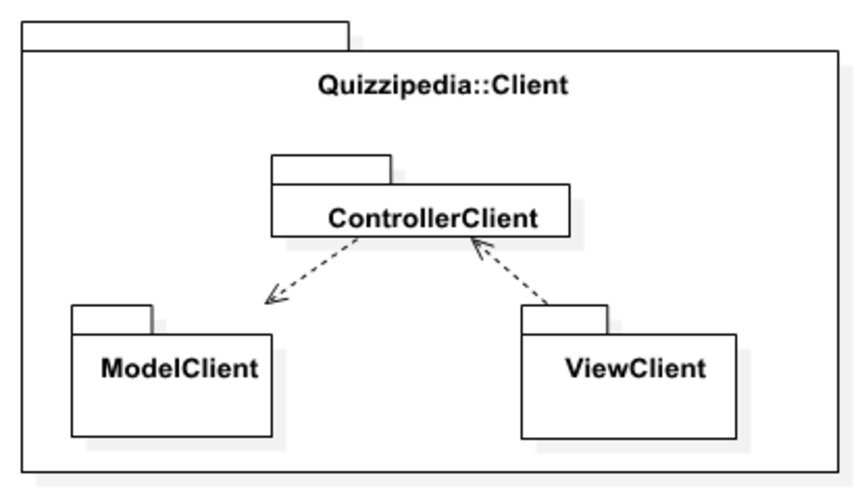
\includegraphics[width=\textwidth]{../SpecificaTecnica/Img/quizzipedia-client.pdf}}
\caption[Schema Componente Client]{Schema Componente Quizzipedia::Client}
\end{figure}
\subsection{\pkg{Quizzipedia::Client::ModelClient}}
Rappresenta il modello dei dati che verranno utilizzati dal sistema lato client. Viene utilizzato tale model per facilitare il recupero di alcune informazioni che altrimenti dovrebbero esser recuperate dal server ogni volta che viene svolta una richiesta dall'utente.
Attraverso l'uso di Angular.js il controller svolge automaticamente le modifiche richieste dalla view nel model in modo tale da tenerlo sempre aggiornato.
\begin{figure}[H]
\centering
\noindent\makebox[\textwidth]{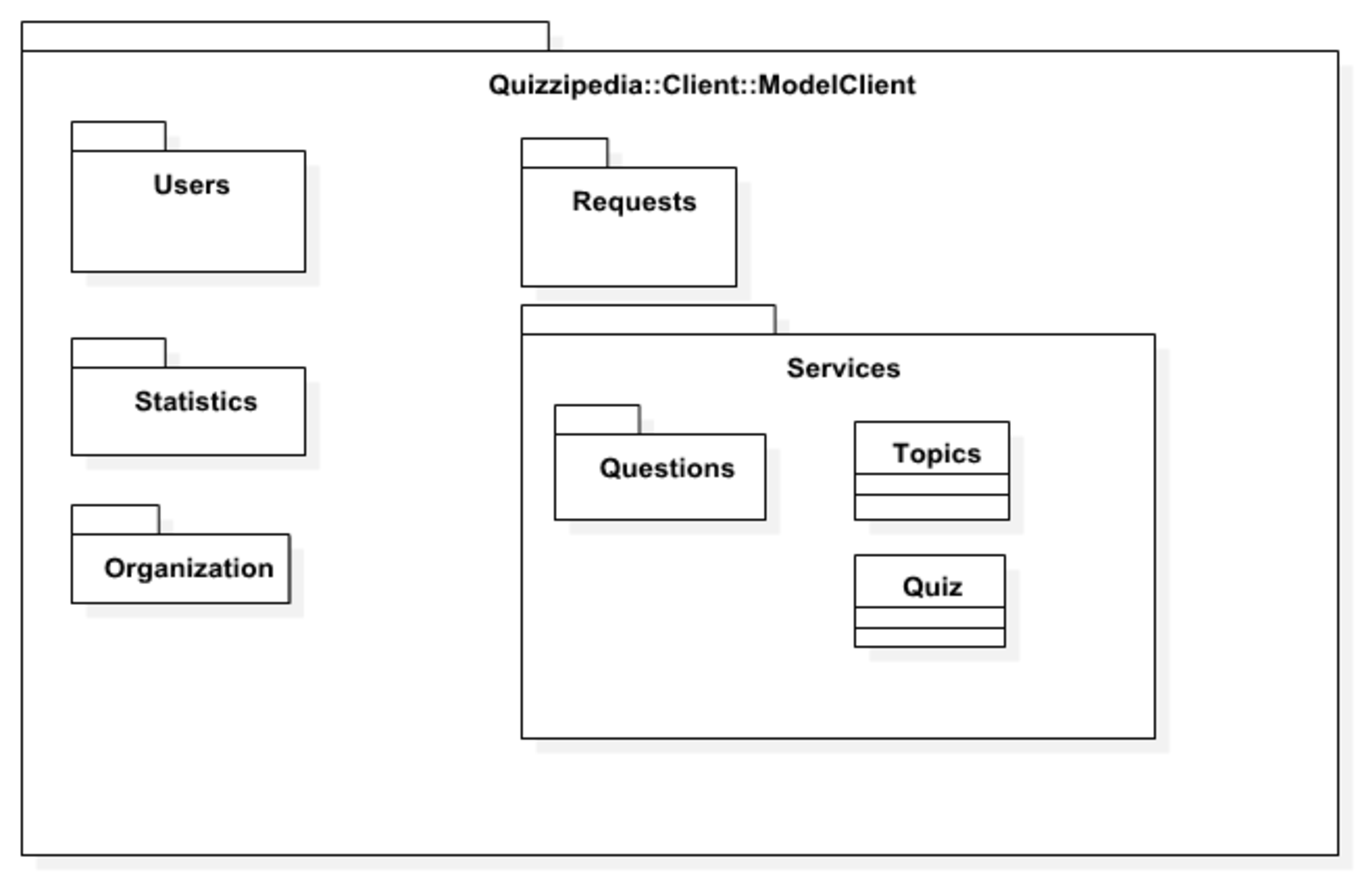
\includegraphics[width=\textwidth]{../SpecificaTecnica/Img/quizzipedia-client-modelclient.pdf}}
\caption[Schema Componente Quizzipedia::Client::ModelClient]{Schema Componente Quizzipedia::Client::ModelClient}
\end{figure}
\subsection{\pkg{Quizzipedia::Client::ModelClient::Organizations}}
La componente gestisce le classi e gli enti, ovvero il sistema in base a cui sono organizzati gli utenti nel sistema.
\begin{figure}[H]
\centering
\noindent\makebox[\textwidth]{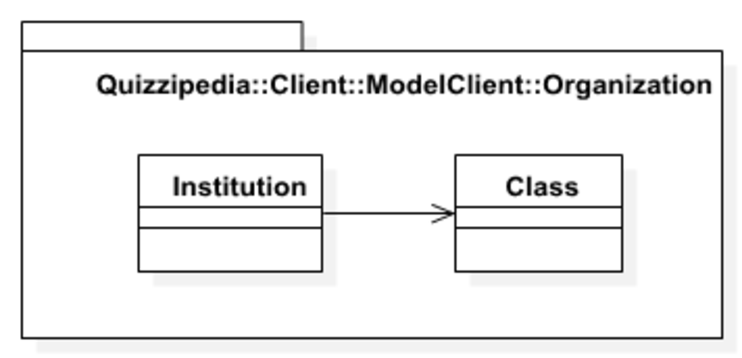
\includegraphics[width=\textwidth]{../SpecificaTecnica/Img/quizzipedia-client-modelclient-organizations.pdf}}
\caption[Schema Componente Quizzipedia::Client::ModelClient::Organizations]{Schema Componente Quizzipedia::Client::ModelClient::Organizations}
\end{figure}
\subsubsection{Classe \cls{Class}}
Rappresenta una classe all'interno di un ente. Memorizza le informazioni che definiscono ogni classe,
informazioni che saranno utilizzate per la visualizzazione e per la gestione della classe stessa.
\begin{figure}[H]
\centering
\noindent\makebox[\textwidth]{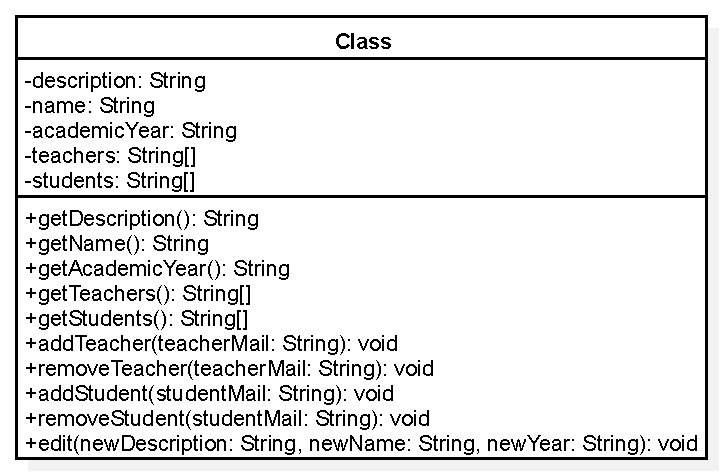
\includegraphics[width=\textwidth]{Img/quizzipedia-client-modelclient-organizations-class.pdf}}
\caption[Schema Classe Class]{Schema Classe Quizzipedia::Client::ModelClient::Organizations::Class}
\end{figure}
\paragraph{Attributi}
\begin{itemize}
\item \attribute{academicYear : String}
\newline
l'anno accademico della classe, per distinguere classi con lo stesso nome
\item \attribute{description : String}
\newline
una breve descrizione della classe
\item \attribute{name : String}
\newline
il nome della classe
\item \attribute{students : String[]}
\newline
le mail degli studenti iscritti alla classe
\item \attribute{teachers : String[]}
\newline
le mail dei docenti associati alla classe
\end{itemize}
\paragraph{Metodi}
\begin{itemize}
\item \method{addStudent () : void}
\newline
permette di aggiungere uno studente alla classe
\newline
\item \method{addTeacher () : void}
\newline
permette di aggiungere un docente alla classe
\newline
\item \method{edit (newDescription : String, newName : String, newYear : String) : void}
\newline
permette
di modificare le informazioni base della classe
\newline
\bold{Parametri} :
\begin{itemize}
\item \attribute{newDescription : String}
\newline
la nuova descrizione della classe
\item \attribute{newName : String}
\newline
il nuovo nome della classe
\item \attribute{newYear : String}
\newline
il nuovo anno della classe
\end{itemize}
\item \method{getAcademicYear () : String}
\newline
restituisce l'anno accademico della classe
\newline
\item \method{getDescription () : String}
\newline
restituisce la descrizione della classe
\newline
\item \method{getName () : String}
\newline
restituisce il nome della classe
\newline
\item \method{getStudents () : String[]}
\newline
restituisce le mail degli studenti della classe
\newline
\item \method{getTeachers () : String[]}
\newline
restituisce le mail dei docenti della classe
\newline
\item \method{removeStudent (studentMail : String) : void}
\newline
permette di rimuovere uno studente dalla
classe
\newline
\bold{Parametri} :
\begin{itemize}
\item \attribute{studentMail : String}
\newline
mail dello studente da rimuovere
\end{itemize}
\item \method{removeTeacher (teacherMail : String) : void}
\newline
permette di rimuovere un docente dalla
classe
\newline
\bold{Parametri} :
\begin{itemize}
\item \attribute{teacherMail : String}
\newline
mail del docente da rimuovere
\end{itemize}
\end{itemize}
\subsubsection{Classe \cls{Institution}}
Tale classe rappresenta un ente. Contiene le informazioni relative alla struttura dell'ente che saranno visualizzate dall'utente e gestiste dal controller, come ad esempio la lista delle classi presenti nell'ente, la lista degli studenti e degli insegnati all'interno dell'ente.
\begin{figure}[H]
\centering
\noindent\makebox[\textwidth]{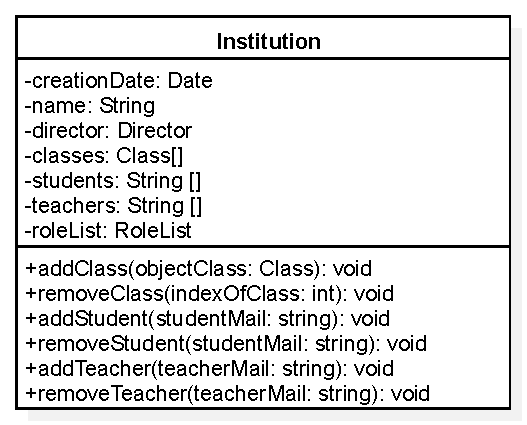
\includegraphics[width=\textwidth]{Img/quizzipedia-client-modelclient-organizations-institution.pdf}}
\caption[Schema Classe Institution]{Schema Classe Quizzipedia::Client::ModelClient::Organizations::Institution}
\end{figure}
\paragraph{Attributi}
\begin{itemize}
\item \attribute{classes : Class[]}
\newline
raccoglie tutte le classi presenti nell'ente
\item \attribute{classList : ClassList}
\newline
le richieste di ingresso ad una classe dell'istituto
\item \attribute{creationDate : Date}
\newline
indica la data di creazione dell'ente
\item \attribute{director : Director}
\newline
il direttore dell'istituto
\item \attribute{name : string}
\newline
il nome dell'ente
\item \attribute{roleList : RoleList}
\newline
rappresenta una lista di tutte le richieste di ruolo pendenti per il dato ente
\item \attribute{students : string[]}
\newline
raccoglie le mail di tutti gli studenti registrati presso un ente
\item \attribute{teachers : string[]}
\newline
raccoglie le mail di tutti i docenti registrati presso un ente
\item \attribute{topics : Topics}
\newline
i topic dell'istituto
\end{itemize}
\paragraph{Metodi}
\begin{itemize}
\item \method{acceptClassRequest (indexOfRequest : int) : void}
\newline
permette di accettare una richiesta di ingresso ad una classe
\newline
\bold{Parametri} :
\begin{itemize}
\item \attribute{indexOfRequest : int}
\newline
la posizione della richiesta di ingresso ad una classe da accettare
\end{itemize}
\item \method{acceptRequestRole (role : String) : void}
\newline
permette di accettare una richiesta di ingresso ad un ruolo dell'istituto
\newline
\bold{Parametri} :
\begin{itemize}
\item \attribute{role : String}
\newline
l'utente da accettare nell'istituto
\end{itemize}
\item \method{addClass  (objectClass : Class) : void}
\newline
Permette l'aggiunta di una classe all'interno di un istituto
\newline
\bold{Parametri} :
\begin{itemize}
\item \attribute{objectClass : Class}
\newline
viene passata al metodo la classe da inserire
\end{itemize}
\item \method{getClass () : Class[]}
\newline
permette di recuperare le classi facenti parte dell'istituto
\newline
\item \method{getCLassList () : ClassList}
\newline
permette di recuperare la lista delle richieste di entrata alle classi
\newline
\item \method{getDirector () : Director}
\newline
permette di recuperare il direttore dell'istittuto
\newline
\item \method{getName () : String}
\newline
permette di recuperare il nome dell'istituto
\newline
\item \method{getRoleList () : RoleList}
\newline
permette di recuperare le richieste di ingresso all'istituto con un appropriato ruolo
\newline
\item \method{getStudents () : String[]}
\newline
permette di recuperare gli studenti abilitati nell'istituto
\newline
\item \method{getTeachers () : String[]}
\newline
permette di recuperare gliinsegnanti abilitati nell'istituto
\newline
\item \method{getTopics () : Topics}
\newline
permette di recuperare i topics dll'istituto
\newline
\item \method{removeClass (indexOfClass : int) : void}
\newline
rimuove una classe da un istituto
\newline
\bold{Parametri} :
\begin{itemize}
\item \attribute{indexOfClass : int}
\newline
l'indice della classe da rimuovere dalle classi presenti nell'ente
\end{itemize}
\item \method{removeClassRequest (indexOfRequest : int) : void}
\newline
permette di rimuovere una richiesta di ingresso ad una classe dell'istituto
\newline
\bold{Parametri} :
\begin{itemize}
\item \attribute{indexOfRequest : int}
\newline
la posizione della richiesta da rimuovere
\end{itemize}
\item \method{removeStudent (studentMail : String) : void}
\newline
rimuove uno studente dagli iscritti presso un istituto
\newline
\bold{Parametri} :
\begin{itemize}
\item \attribute{studentMail : String}
\newline
lo studente da rimuovere dall'istituto
\end{itemize}
\item \method{removeTeacher (teacherMail : String) : void}
\newline
rimuove un docente dagli iscritti presso un istituto
\newline
\bold{Parametri} :
\begin{itemize}
\item \attribute{teacherMail : String}
\newline
l'insegnate da rimuovere dall'istituto
\end{itemize}
\item \method{setDirector (objectDirector : Director) : void}
\newline
permette di modificare il direttore dell'istituto
\newline
\bold{Parametri} :
\begin{itemize}
\item \attribute{objectDirector : Director}
\newline
il nuovo direttore dell'istituto
\end{itemize}
\item \method{setName (newName : String) : void}
\newline
permette di modificare il nome dell'istituto
\newline
\bold{Parametri} :
\begin{itemize}
\item \attribute{newName : String}
\newline
il nuovo nome dell'istituto
\end{itemize}
\end{itemize}
\subsection{\pkg{Quizzipedia::Client::ModelClient::Requests}}
Questo componente contiene le classi necessarie a gestire le richieste di ruolo e di classe degli utenti autenticati.
\begin{figure}[H]
\centering
\noindent\makebox[\textwidth]{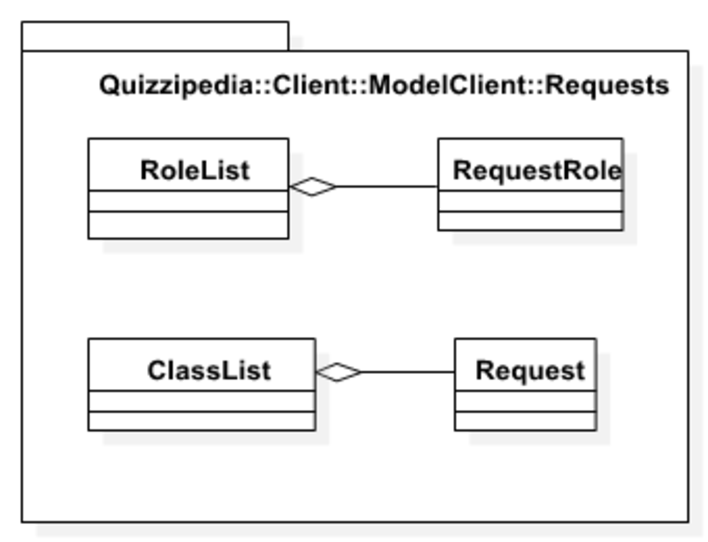
\includegraphics[width=\textwidth]{../SpecificaTecnica/Img/quizzipedia-client-modelclient-requests.pdf}}
\caption[Schema Componente Quizzipedia::Client::ModelClient::Requests]{Schema Componente Quizzipedia::Client::ModelClient::Requests}
\end{figure}
\subsubsection{Classe \cls{ClassList}}
Questa classe gestisce le richieste da parte di docenti o studenti per l'assegnazione a una specifica classe. Contiene i metodi da cui è possibile accettare o rifiutare la richiesta dell'utente.
\begin{figure}[H]
\centering
\noindent\makebox[\textwidth]{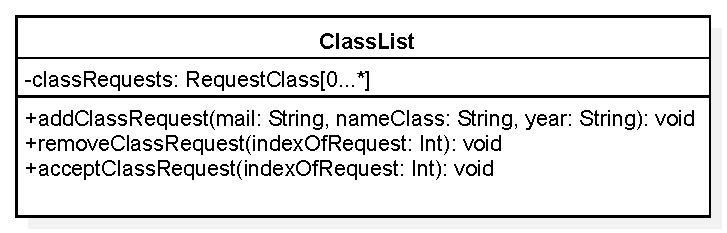
\includegraphics[width=\textwidth]{Img/quizzipedia-client-modelclient-requests-classlist.pdf}}
\caption[Schema Classe ClassList]{Schema Classe Quizzipedia::Client::ModelClient::Requests::ClassList}
\end{figure}
\paragraph{Attributi}
\begin{itemize}
\item \attribute{classRequest : RequestClass[]}
\newline
è la lista delle richieste di classe pendenti
\end{itemize}
\paragraph{Metodi}
\begin{itemize}
\item \method{acceptClassRequest (indexOfRequest : int) : void}
\newline
accetta la richiesta di entrata in una classe dell'utente
\newline
\bold{Parametri} :
\begin{itemize}
\item \attribute{indexOfRequest : int}
\newline
è l'indice della richiesta che si intende accettare
\end{itemize}
\item \method{addClassRequest (mail : String, nameClass : String, year : String) : void}
\newline
aggiunge una richiesta di entrata in una classe alla lista delle richieste pendenti
\newline
\bold{Parametri} :
\begin{itemize}
\item \attribute{mail : String}
\newline
la mail dell'utente che effettua la richiesta di entrata nella classe
\item \attribute{nameClass : String}
\newline
il nome della classe per cui si sta effettuando la richiesta
\item \attribute{year : String}
\newline
l'anno della classe per cui si sta effettuando la richiesta
\end{itemize}
\item \method{removeClassRequest (indexOfRequest : int) : void}
\newline
rimuove una richiesta di entrata nella classe dalla lista delle richieste pendenti. Di fatto, comporta il rifiuto della richiesta
\newline
\bold{Parametri} :
\begin{itemize}
\item \attribute{indexOfRequest : int}
\newline
l'indice della richiesta che si intende rifiutare e rimuovere dalla lista
\end{itemize}
\end{itemize}
\subsubsection{Classe \cls{RequestClass}}
La classe memorizza l'utente che invia la richiesta di inserimento in una classe e la classe per cui la richiesta è stata effettuata.
\begin{figure}[H]
\centering
\noindent\makebox[\textwidth]{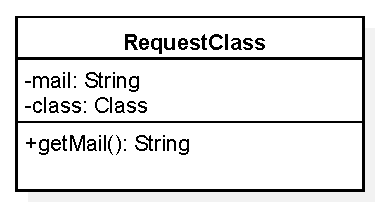
\includegraphics[width=\textwidth]{Img/quizzipedia-client-modelclient-requests-requestclass.pdf}}
\caption[Schema Classe RequestClass]{Schema Classe Quizzipedia::Client::ModelClient::Requests::RequestClass}
\end{figure}
\paragraph{Attributi}
\begin{itemize}
\item \attribute{class : Class}
\newline
la classe per cui è stata effettuata la richiesta
\item \attribute{mail : String}
\newline
la mail dell'utente che ha effettuato la richiesta
\end{itemize}
\paragraph{Metodi}
\begin{itemize}
\item \method{getMail () : String}
\newline
restituisce la mail dell'utente che ha effettuato la richiesta
\newline
\end{itemize}
\subsubsection{Classe \cls{RequestRole}}
La classe memorizza l'utente che invia una richiesta di ruolo e il ruolo che vuole ricoprire.
\begin{figure}[H]
\centering
\noindent\makebox[\textwidth]{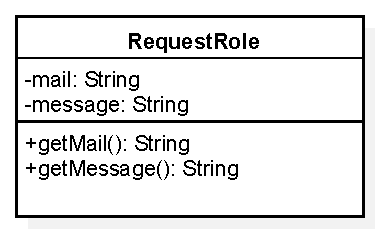
\includegraphics[width=\textwidth]{Img/quizzipedia-client-modelclient-requests-requestrole.pdf}}
\caption[Schema Classe RequestRole]{Schema Classe Quizzipedia::Client::ModelClient::Requests::RequestRole}
\end{figure}
\paragraph{Attributi}
\begin{itemize}
\item \attribute{mail : String}
\newline
la mail dell'utente che effettua la richiesta di ruolo
\item \attribute{messagge : String}
\newline
un messaggio che l'utente può includere alla sua richiesta di ruolo
\end{itemize}
\paragraph{Metodi}
\begin{itemize}
\item \method{getMail () : String}
\newline
restituisce la mail dell'utente che effettua la richiesta
\newline
\item \method{getMessage () : String}
\newline
restituisce il messaggio dell'utente che effettua la richista
\newline
\end{itemize}
\subsubsection{Classe \cls{RoleList}}
Gli utenti senza ruolo inviano le proprie richieste per l'assegnazione al ruolo di studente o docente al responsabile di un ente. Questa classe gestisce tali richieste.
\begin{figure}[H]
\centering
\noindent\makebox[\textwidth]{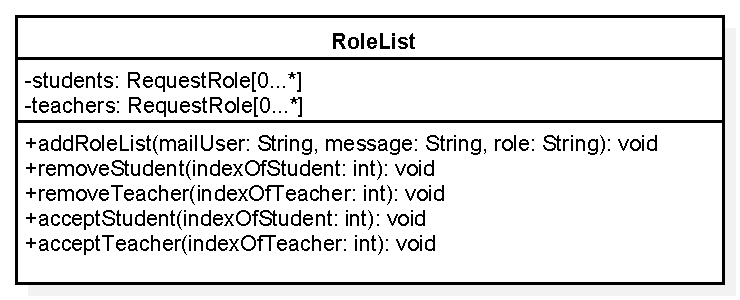
\includegraphics[width=\textwidth]{Img/quizzipedia-client-modelclient-requests-rolelist.pdf}}
\caption[Schema Classe RoleList]{Schema Classe Quizzipedia::Client::ModelClient::Requests::RoleList}
\end{figure}
\paragraph{Attributi}
\begin{itemize}
\item \attribute{students : RequesRole[]}
\newline
memorizza la lista delle richieste degli utenti che hanno richiesto di diventare studenti
\item \attribute{teachers : RequestRole[]}
\newline
memorizza la lista delle richieste degli utenti che hanno richiesto di diventare docenti
\end{itemize}
\paragraph{Metodi}
\begin{itemize}
\item \method{acceptStudent (indexOfStudent : int) : void}
\newline
accetta la richiesta di ruolo di un utente senza ruolo che desidera diventare studente
\newline
\bold{Parametri} :
\begin{itemize}
\item \attribute{indexOfStudent : int}
\newline
l'indice della richiesta di ruolo che si intende accettare. L'utente diventa uno studente dell'ente
\end{itemize}
\item \method{acceptTeacher (indexOfTeacher : int) : void}
\newline
accetta la richiesta di ruolo di un utente senza ruolo che desidera diventare docente
\newline
\bold{Parametri} :
\begin{itemize}
\item \attribute{indexOfTeacher : int}
\newline
l'indice della richiesta di ruolo che si intende accettare. L'utente diventa un docente dell'ente
\end{itemize}
\item \method{addRoleList (mailUser : String, message : String, role : String) : void}
\newline
il metodo aggiunge una richiesta alla lista corretta delle richieste pendenti
\newline
\bold{Parametri} :
\begin{itemize}
\item \attribute{mailUser : String}
\newline
la mail dell'utente che ha effettuato una richiesta di ruolo
\item \attribute{message : String}
\newline
il messaggio dell'utente che ha effettuato una richiesta di ruolo
\item \attribute{role : String}
\newline
il ruolo per cui l'utente ha fatto domanda
\end{itemize}
\item \method{removeStudent () : void}
\newline
rimuove, quindi rifiutandola, la richiesta di ruolo di un utente senza ruolo che desidera diventare studente
\newline
\item \method{removeTeacher () : void}
\newline
rimuove, quindi rifiutandola, la richiesta di ruolo di un utente senza ruolo che desidera diventare studente
\newline
\end{itemize}
\subsection{\pkg{Quizzipedia::Client::ModelClient::Services}}
Il componente racchiude i modelli necessari alla creazione di domande e quiz, i servizi principali offerti dal nostro prodotto.
\begin{figure}[H]
\centering
\noindent\makebox[\textwidth]{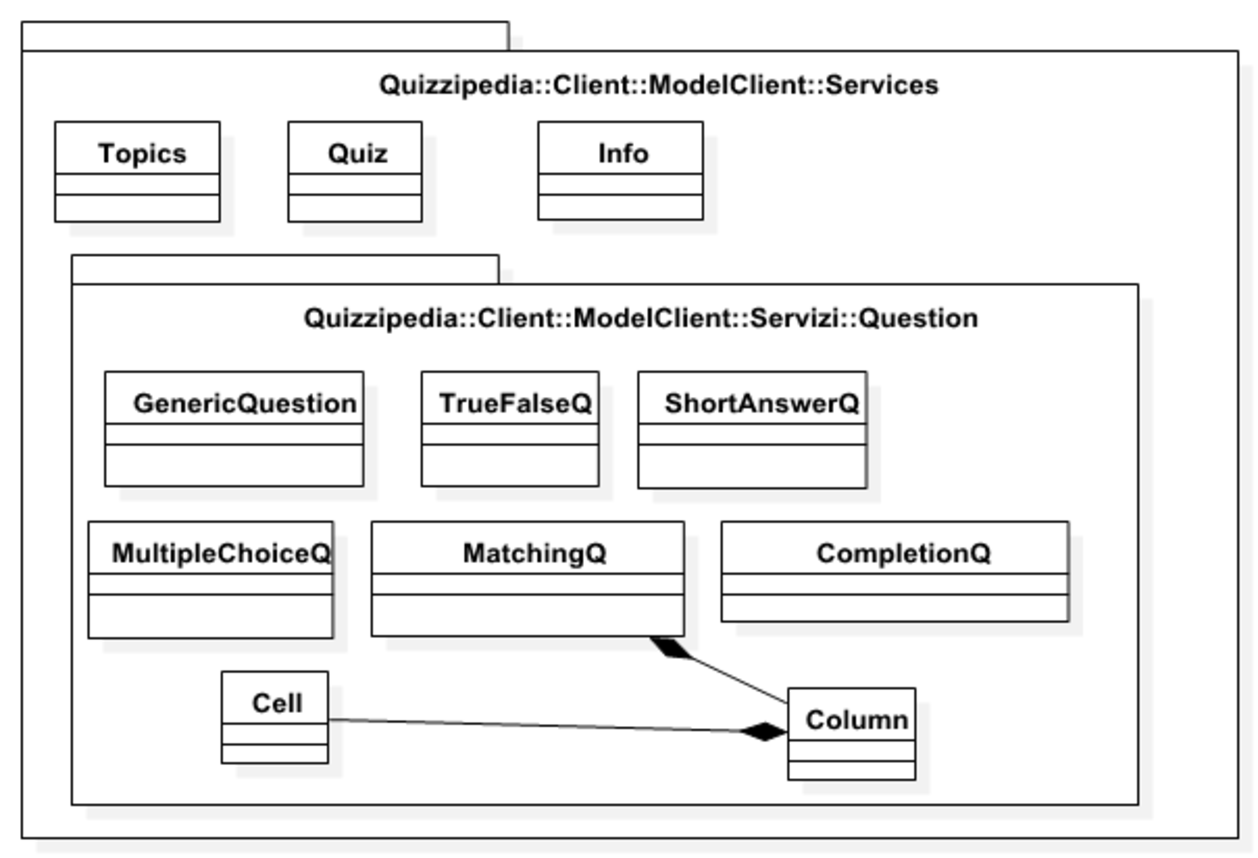
\includegraphics[width=\textwidth]{../SpecificaTecnica/Img/quizzipedia-client-modelclient-services.pdf}}
\caption[Schema Componente Quizzipedia::Client::ModelClient::Services]{Schema Componente Quizzipedia::Client::ModelClient::Services}
\end{figure}
\subsubsection{Classe \cls{Quiz}}
Include la struttura del quiz.
\begin{figure}[H]
\centering
\noindent\makebox[\textwidth]{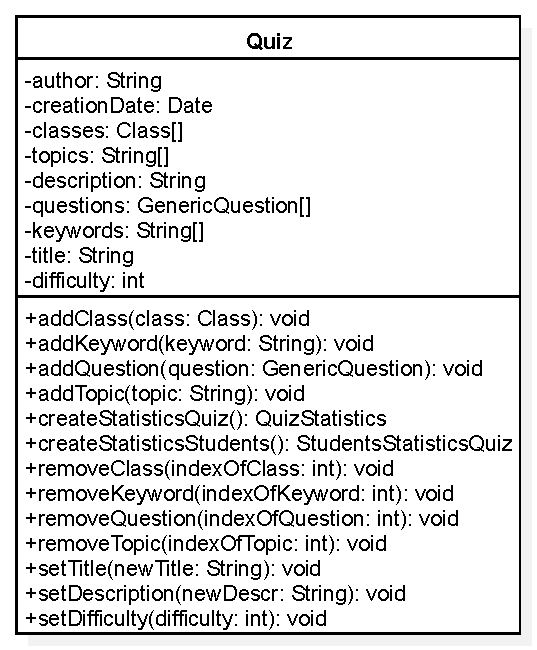
\includegraphics[width=\textwidth]{Img/quizzipedia-client-modelclient-services-quiz.pdf}}
\caption[Schema Classe Quiz]{Schema Classe Quizzipedia::Client::ModelClient::Services::Quiz}
\end{figure}
\paragraph{Attributi}
\begin{itemize}
\item \attribute{author : String}
\newline
la mail del docente che ha creato il quiz
\item \attribute{classes : Class[]}
\newline
la lista delle classi per cui il quiz è stato creato
\item \attribute{creationDate : Date}
\newline
la data di creazione del quiz
\item \attribute{description : String}
\newline
la descrizione del quiz
\item \attribute{keywords : String[]}
\newline
le keyword che identificano il quiz
\item \attribute{questions : GenericQuestion[]}
\newline
La lista delle domande che compongono il quiz
\item \attribute{title : String}
\newline
il titolo del quiz
\item \attribute{topics : String[]}
\newline
gli argomenti coperti dal quiz
\end{itemize}
\paragraph{Metodi}
\begin{itemize}
\item \method{addClass (class : Class) : void}
\newline
aggiunge una classe alla lista delle classi che hanno accesso al quiz
\newline
\bold{Parametri} :
\begin{itemize}
\item \attribute{class : Class}
\newline
la classe che si intende aggiungere
\end{itemize}
\item \method{addKeyword (keyword : String) : void}
\newline
aggiunge una parola chiave per identificare il quiz
\newline
\bold{Parametri} :
\begin{itemize}
\item \attribute{keyword : String}
\newline
la parola chiave da aggiungere
\end{itemize}
\item \method{addQuestion (question : GenericQuestion) : void}
\newline
aggiunge una domanda al quiz
\newline
\bold{Parametri} :
\begin{itemize}
\item \attribute{question : GenericQuestion}
\newline
la domanda da aggiungere al quiz
\end{itemize}
\item \method{addTopic (topic : String) : void}
\newline
aggiunge un argomento agli argomenti del quiz
\newline
\bold{Parametri} :
\begin{itemize}
\item \attribute{topic : String}
\newline
l'argomento da aggiungere
\end{itemize}
\item \method{createStatisticsQuiz () : QuizStatistics}
\newline
restituisce un oggetto contenente le statistiche generali del quiz
\newline
\item \method{createStatisticsStudents () : StudentsStatisticsQuiz}
\newline
ritorna un oggetto contenente le statistiche degli utenti che hanno risolto il quiz
\newline
\item \method{removeClass (indexOfClass : int) : void}
\newline
rimuove una classe da quelle che hanno accesso al quiz. Rimuovendo tutte le classi il quiz diventa pubblico
\newline
\bold{Parametri} :
\begin{itemize}
\item \attribute{indexOfClass : int}
\newline
l'indice della classe da rimuovere
\end{itemize}
\item \method{removeKeyword (indexOfKeyword : int) : void}
\newline
rimuove una parola chiave da quelle che identificano il quiz
\newline
\bold{Parametri} :
\begin{itemize}
\item \attribute{indexOfKeyword : int}
\newline
l'indice della parola chiave da rimuovere
\end{itemize}
\item \method{removeQuestion (indexOfQuestion : int) : void}
\newline
rimuove una domanda dal quiz
\newline
\bold{Parametri} :
\begin{itemize}
\item \attribute{indexOfQuestion : int}
\newline
l'indice della domanda da rimuovere
\end{itemize}
\item \method{removeTopic (indexOfTopic : int) : void}
\newline
rimuove un argomento da quelli che identificano il quiz
\newline
\bold{Parametri} :
\begin{itemize}
\item \attribute{indexOfTopic : int}
\newline
l'indice della classe da rimuovere
\end{itemize}
\item \method{setDescription (newDescr : String) : void}
\newline
imposta la descrizione del quiz
\newline
\bold{Parametri} :
\begin{itemize}
\item \attribute{newDescr : String}
\newline
la nuova descrizione del quiz
\end{itemize}
\item \method{setTitle (newTitle : String) : void}
\newline
imposta il titolo del quiz
\newline
\bold{Parametri} :
\begin{itemize}
\item \attribute{newTitle : String}
\newline
il nuovo titolo del quiz
\end{itemize}
\end{itemize}
\subsubsection{Classe \cls{Topics}}
Modella la struttura necessaria a memorizzare la lista di argomenti. A ogni domanda e a ogni quiz verranno poi associati i relativi argomenti .
\begin{figure}[H]
\centering
\noindent\makebox[\textwidth]{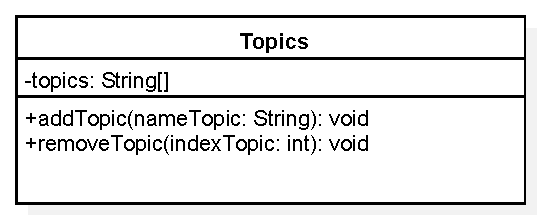
\includegraphics[width=\textwidth]{Img/quizzipedia-client-modelclient-services-topics.pdf}}
\caption[Schema Classe Topics]{Schema Classe Quizzipedia::Client::ModelClient::Services::Topics}
\end{figure}
\paragraph{Attributi}
\begin{itemize}
\item \attribute{topics : String[]}
\newline
la lista degli argomenti esistenti
\end{itemize}
\paragraph{Metodi}
\begin{itemize}
\item \method{addTopics (nameTopic : String) : void}
\newline
permettere di aggiungere un nuovo argomento a quelli esistenti
\newline
\bold{Parametri} :
\begin{itemize}
\item \attribute{nameTopic : String}
\newline
il nuovo argomento da aggiungere
\end{itemize}
\item \method{removeTopic (indexTopic : int) : void}
\newline
permette di rimuovere un argomento da quelli esistenti
\newline
\bold{Parametri} :
\begin{itemize}
\item \attribute{indexTopic : int}
\newline
l'indice dell'argomento da rimuovere
\end{itemize}
\end{itemize}
\subsection{\pkg{Quizzipedia::Client::ModelClient::Services::Answers}}
Raccoglie tutte le componenti necessarie alla gestione della verifica dei quiz e delle domande svolte.
\begin{figure}[H]
\centering
\noindent\makebox[\textwidth]{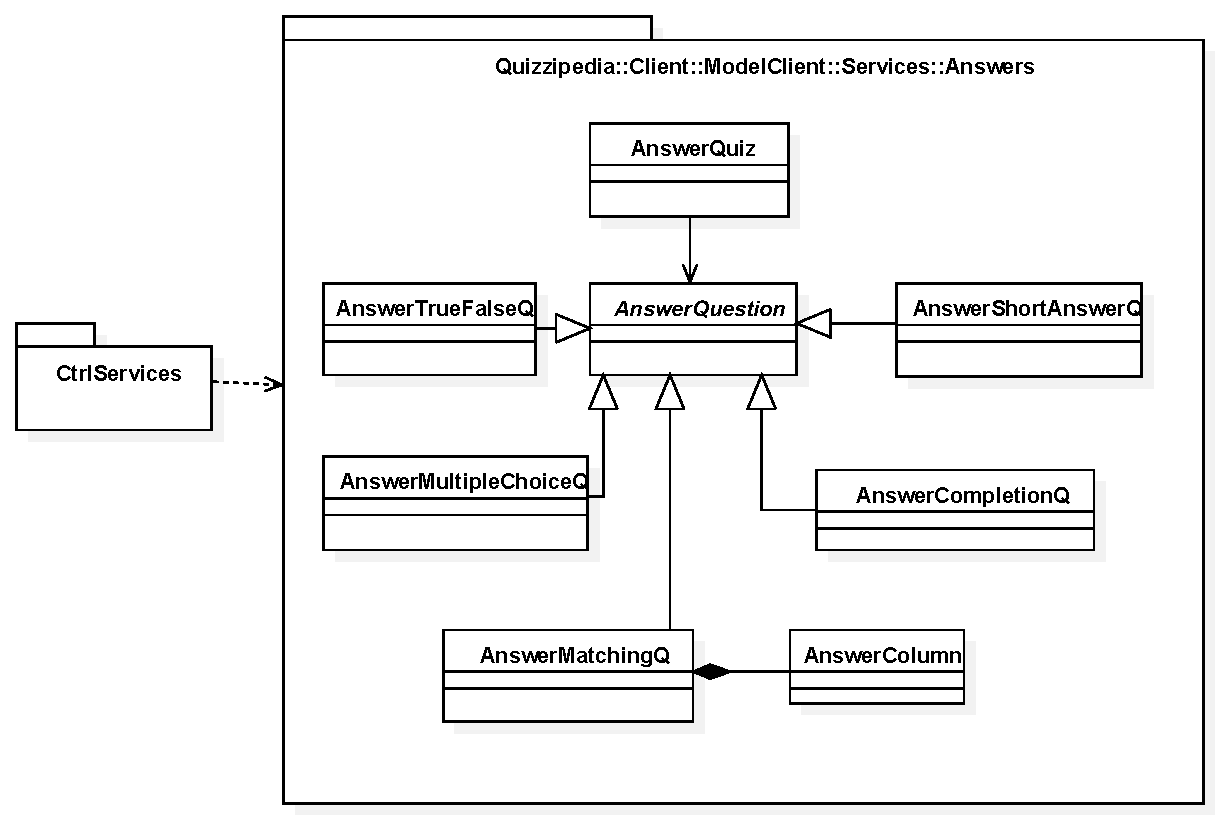
\includegraphics[width=\textwidth]{../SpecificaTecnica/Img/quizzipedia-client-modelclient-services-answers.pdf}}
\caption[Schema Componente Quizzipedia::Client::ModelClient::Services::Answers]{Schema Componente Quizzipedia::Client::ModelClient::Services::Answers}
\end{figure}
\subsubsection{Classe \cls{AnswerColumn}}
Classe utilizzata da AnswerMatchingQ per salvare le risposte della domanda MatchingQ.
\begin{figure}[H]
\centering
\noindent\makebox[\textwidth]{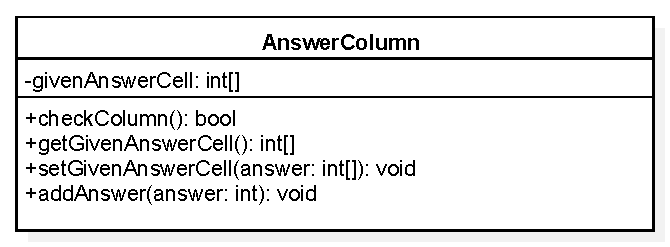
\includegraphics[width=\textwidth]{Img/quizzipedia-client-modelclient-services-answers-answercolumn.pdf}}
\caption[Schema Classe AnswerColumn]{Schema Classe Quizzipedia::Client::ModelClient::Services::Answers::AnswerColumn}
\end{figure}
\paragraph{Attributi}
\begin{itemize}
\item \attribute{givenAnswerCell : int[]}
\newline
le risposte date dall'utente in una colonna della domanda a collegamenti
\end{itemize}
\paragraph{Metodi}
\begin{itemize}
\item \method{checkColumn () : bool}
\newline
verifica l correttezza di una colonna data la risposta a una domanda a collegamenti
\newline
\item \method{getGivenAnswerCell () : int[]}
\newline
restituisce le risposte date dall'utente in una colonna della domanda a collegamento
\newline
\item \method{setGivenAnswerCell (answer : int[]) : void}
\newline
imposta, memorizzando correttamente, le risposte date dall'utente in una colonna della domanda a collegamenti
\newline
\bold{Parametri} :
\begin{itemize}
\item \attribute{answer : int[]}
\newline
la risposta data dall'utente che verrà memorizzata
\end{itemize}
\end{itemize}
\subsubsection{Classe \cls{AnswerCompletionQ}}
Classe che si occupa di memorizzare le informazioni di un domanda CompletionQ risolta.
\begin{figure}[H]
\centering
\noindent\makebox[\textwidth]{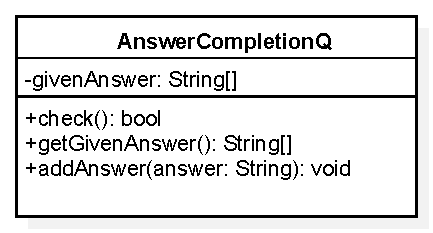
\includegraphics[width=\textwidth]{Img/quizzipedia-client-modelclient-services-answers-answercompletionq.pdf}}
\caption[Schema Classe AnswerCompletionQ]{Schema Classe Quizzipedia::Client::ModelClient::Services::Answers::AnswerCompletionQ}
\end{figure}
\paragraph{Attributi}
\begin{itemize}
\item \attribute{givenAnswer : String[]}
\newline
la risposta data dall'utente
\end{itemize}
\paragraph{Metodi}
\begin{itemize}
\item \method{check () : bool}
\newline
concretizzazione del metodo ereditato dalla classe base astratta. Viene implementato in modo che verifichi la correttezza della risposta al fronte di una domanda a completamento
\newline
\item \method{getGivenAnswer () : String[]}
\newline
restituisce la risposta data dall'utente
\newline
\end{itemize}
\subsubsection{Classe \cls{AnswerMatchingQ}}
Classe che si occupa di memorizzare le informazioni di un domanda MatchingQ risolta.
\begin{figure}[H]
\centering
\noindent\makebox[\textwidth]{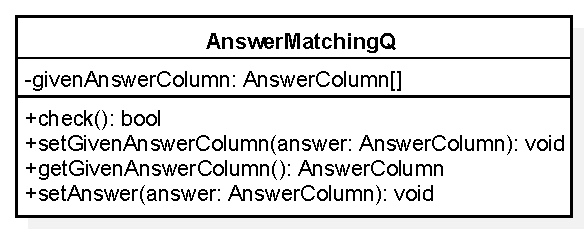
\includegraphics[width=\textwidth]{Img/quizzipedia-client-modelclient-services-answers-answermatchingq.pdf}}
\caption[Schema Classe AnswerMatchingQ]{Schema Classe Quizzipedia::Client::ModelClient::Services::Answers::AnswerMatchingQ}
\end{figure}
\paragraph{Attributi}
\begin{itemize}
\item \attribute{givenAnswerColumn : AnswerColumn[]}
\newline
le risposte data dall'utente per le varie colonne della domanda a collegamenti
\end{itemize}
\paragraph{Metodi}
\begin{itemize}
\item \method{check () : bool}
\newline
concretizzazione del metodo ereditato dalla classe base astratta. Viene implementato in modo che verifichi la correttezza della risposta al fronte di una domanda a collegamenti
\newline
\item \method{getGivenAnswerColumn () : AnswerColumn}
\newline
restituisce le risposte date dall'utente per una delle colonne della domanda a collegamenti
\newline
\item \method{setGivenAnswerColumn (answer : AnswerColumn) : void}
\newline
imposta le risposte date dall'utente per una delle colonne della domanda a collegamenti
\newline
\bold{Parametri} :
\begin{itemize}
\item \attribute{answer : AnswerColumn}
\newline
le risposte date dall'utente per una delle colonne della domanda a collegnamenti
\end{itemize}
\end{itemize}
\subsubsection{Classe \cls{AnswerMultipleChoiceQ}}
Classe che si occupa di memorizzare le informazioni di un domanda MultipleChoiceQ risolta.
\begin{figure}[H]
\centering
\noindent\makebox[\textwidth]{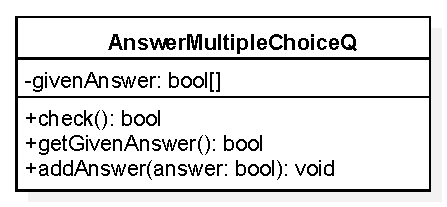
\includegraphics[width=\textwidth]{Img/quizzipedia-client-modelclient-services-answers-answermultiplechoiceq.pdf}}
\caption[Schema Classe AnswerMultipleChoiceQ]{Schema Classe Quizzipedia::Client::ModelClient::Services::Answers::AnswerMultipleChoiceQ}
\end{figure}
\paragraph{Attributi}
\begin{itemize}
\item \attribute{givenAnswer : bool[]}
\newline
la risposta data dall'utente
\end{itemize}
\paragraph{Metodi}
\begin{itemize}
\item \method{check () : bool}
\newline
concretizzazione del metodo ereditato dalla classe base astratta. Viene implementato in modo che verifichi la correttezza della risposta al fronte di una domanda a acelta multipla
\newline
\item \method{getGivenAnswer () : bool[]}
\newline
restituisce la risposta data dall'utente
\newline
\end{itemize}
\subsubsection{Classe \cls{AnswerQuestion}}
Classe che si occupa di memorizzare le informazioni di un domanda risolta.
\begin{figure}[H]
\centering
\noindent\makebox[\textwidth]{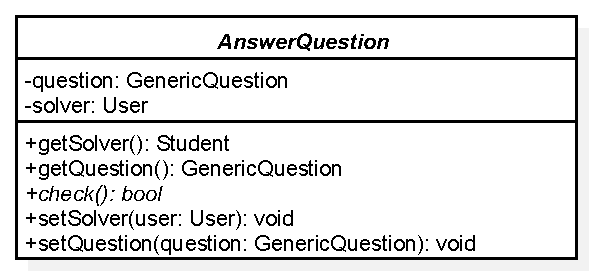
\includegraphics[width=\textwidth]{Img/quizzipedia-client-modelclient-services-answers-answerquestion.pdf}}
\caption[Schema Classe AnswerQuestion]{Schema Classe Quizzipedia::Client::ModelClient::Services::Answers::AnswerQuestion}
\end{figure}
\paragraph{Attributi}
\begin{itemize}
\item \attribute{question : GenericQuestion}
\newline
la domanda a cui corrisponde la risposta data
\end{itemize}
\paragraph{Metodi}
\begin{itemize}
\item \method{<<abstract>>check () : bool}
\newline
il metodo è astratto e verrà concretizzato nelle sottoclassi. Serve a verificare la correttezza della risposta data per le varie tipologie di domande
\newline
\item \method{getQuestion () : GenricQuestion}
\newline
restituisce la domanda a cui corrisponde la risposta data
\newline
\end{itemize}
\subsubsection{Classe \cls{AnswerQuiz}}
Classe che si occupa di memorizzare le informazioni di un quiz completato e gestisce la verifica del suo superamento.
\begin{figure}[H]
\centering
\noindent\makebox[\textwidth]{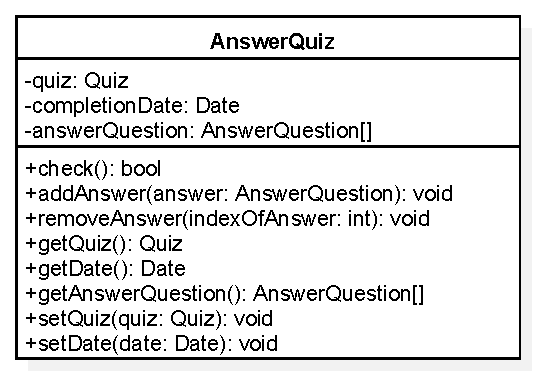
\includegraphics[width=\textwidth]{Img/quizzipedia-client-modelclient-services-answers-answerquiz.pdf}}
\caption[Schema Classe AnswerQuiz]{Schema Classe Quizzipedia::Client::ModelClient::Services::Answers::AnswerQuiz}
\end{figure}
\paragraph{Attributi}
\begin{itemize}
\item \attribute{answerQuestion : AnswerQuestion[]}
\newline
sono le risposte date alle singole domande che compongono il quiz
\item \attribute{completionDate : Date}
\newline
la data di risoluzione del quiz
\item \attribute{quiz : Quiz}
\newline
è il Quiz a cui sono associate le risposte date dall'utente
\end{itemize}
\paragraph{Metodi}
\begin{itemize}
\item \method{addAnswer (answer : AnswerQuestion) : void}
\newline
aggiunge la risposta a una delle domande del quiz alla lista delle risposte per il quiz corrente
\newline
\bold{Parametri} :
\begin{itemize}
\item \attribute{answer : AnswerQuestion}
\newline
la risposta da aggiungere alla lista delle risposte del quiz
\end{itemize}
\item \method{check () : bool}
\newline
verifica la correttezza del quiz, confrontando le risposte date dall'utente con quelle corrette
\newline
\item \method{getAnswerQuestion () : AnswerQuestion}
\newline
restituisce la lista delle risposte alle varie domande del quiz
\newline
\item \method{getDate () : Date}
\newline
restituisce la data in cui il quiz è stato risolto
\newline
\item \method{getQuiz () : Quiz}
\newline
restituisce il Quiz che l'utente sta risolvendo
\newline
\item \method{removeAnswer (indexOfAnswer : int) : void}
\newline
rimuove la risposta data dall'utente a una domanda dalla lista delle risposte alle domande del quiz corrente
\newline
\bold{Parametri} :
\begin{itemize}
\item \attribute{indexOfAnswer : int}
\newline
l'indice della risposta da rimuovere dalla lista di risposte alle domande del quiz
\end{itemize}
\end{itemize}
\subsubsection{Classe \cls{AnswerShortAnswerQ}}
Classe che si occupa di memorizzare le informazioni di un domanda ShortAnswerQ risolta.
\begin{figure}[H]
\centering
\noindent\makebox[\textwidth]{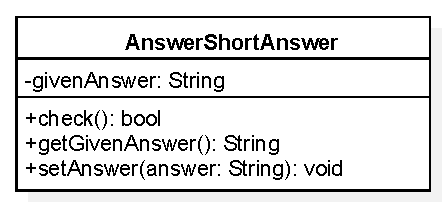
\includegraphics[width=\textwidth]{Img/quizzipedia-client-modelclient-services-answers-answershortanswerq.pdf}}
\caption[Schema Classe AnswerShortAnswerQ]{Schema Classe Quizzipedia::Client::ModelClient::Services::Answers::AnswerShortAnswerQ}
\end{figure}
\paragraph{Attributi}
\begin{itemize}
\item \attribute{givenAnswer : String}
\newline
la risposta data dall'utente
\end{itemize}
\paragraph{Metodi}
\begin{itemize}
\item \method{check () : bool}
\newline
concretizzazione del metodo ereditato dalla classe base astratta. Viene implementato in modo che verifichi la correttezza della risposta al fronte di una domanda aperta
\newline
\item \method{getGivenAnswer () : String}
\newline
restituisce la risposta dell'utente
\newline
\end{itemize}
\subsubsection{Classe \cls{AnswerTrueFalseQ}}
Classe che si occupa di memorizzare le informazioni di un domanda TrueFalseQ risolta.
\begin{figure}[H]
\centering
\noindent\makebox[\textwidth]{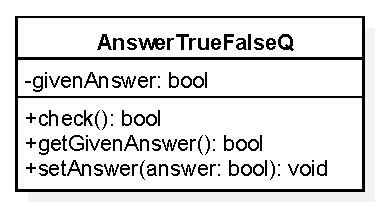
\includegraphics[width=\textwidth]{Img/quizzipedia-client-modelclient-services-answers-answertruefalseq.pdf}}
\caption[Schema Classe AnswerTrueFalseQ]{Schema Classe Quizzipedia::Client::ModelClient::Services::Answers::AnswerTrueFalseQ}
\end{figure}
\paragraph{Attributi}
\begin{itemize}
\item \attribute{givenAnswer : bool}
\newline
la risposta data dall'utente alla domanda di tipo vero/falso
\end{itemize}
\paragraph{Metodi}
\begin{itemize}
\item \method{check () : bool}
\newline
concretizzazione del metodo ereditato dalla classe base astratta. Viene implementato in modo che verifichi la correttezza della risposta al fronte di una domanda di tipo vero/falso
\newline
\item \method{getGivenAnswer () : bool}
\newline
restituisce la risposta data dall'utente
\newline
\end{itemize}
\subsection{\pkg{Quizzipedia::Client::ModelClient::Services::Questions}}
Descrive il modo in cui sono strutturati i vari tipi di domande che l'utente può incontrare durante la creazione o la compilazione di quiz.
\begin{figure}[H]
\centering
\noindent\makebox[\textwidth]{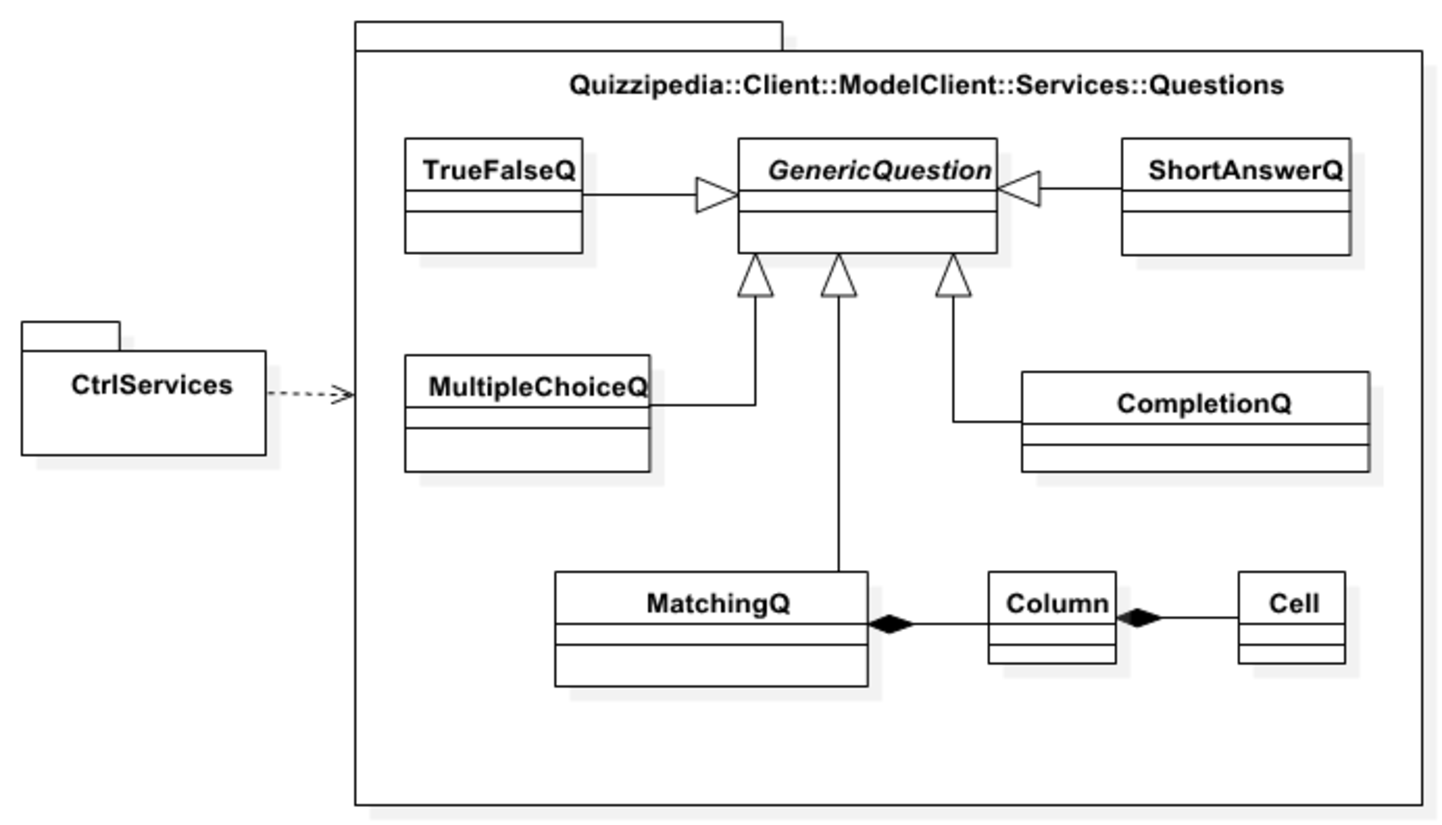
\includegraphics[width=\textwidth]{../SpecificaTecnica/Img/quizzipedia-client-modelclient-services-questions.pdf}}
\caption[Schema Componente Quizzipedia::Client::ModelClient::Services::Questions]{Schema Componente Quizzipedia::Client::ModelClient::Services::Questions}
\end{figure}
\subsubsection{Classe \cls{Cell}}
La classe descrive ogni singola riga (quindi ogni opzione) della colonna della domanda a collegamento.
\begin{figure}[H]
\centering
\noindent\makebox[\textwidth]{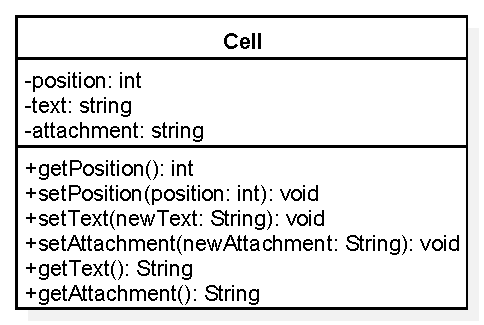
\includegraphics[width=\textwidth]{Img/quizzipedia-client-modelclient-services-questions-cell.pdf}}
\caption[Schema Classe Cell]{Schema Classe Quizzipedia::Client::ModelClient::Services::Questions::Cell}
\end{figure}
\paragraph{Attributi}
\begin{itemize}
\item \attribute{attachment : String}
\newline
l'allegato contenuto nella cella
\item \attribute{position : int}
\newline
la posizione corretta della cella
\item \attribute{text : String}
\newline
il testo contenuto nella cella
\end{itemize}
\paragraph{Metodi}
\begin{itemize}
\item \method{getAttachment () : String}
\newline
permette di recuperare l'allegato della cella
\newline
\item \method{getPosition () : int}
\newline
permette di recuperare la posizione corretta della cella
\newline
\item \method{getText () : String}
\newline
permette di recuperare il testo della cella
\newline
\item \method{setAttachment (newAttachment : String) : void}
\newline
permette di sostituire l'allegato della cella
\newline
\bold{Parametri} :
\begin{itemize}
\item \attribute{newAttachment : String}
\newline
il nuovo allegato da inserire nella cella
\end{itemize}
\item \method{setPosition (position : int) : void}
\newline
permette di modificare la posizione corretta della cella
\newline
\bold{Parametri} :
\begin{itemize}
\item \attribute{position : int}
\newline
la nuova posizione da dare alla cella
\end{itemize}
\item \method{setText (newText : String) : void}
\newline
permette di modificare il testo della cella
\newline
\bold{Parametri} :
\begin{itemize}
\item \attribute{newText : String}
\newline
il nuovo test da inserire nella cella
\end{itemize}
\end{itemize}
\subsubsection{Classe \cls{Column}}
La classe descrive le colonne della domanda a collegamenti.
\begin{figure}[H]
\centering
\noindent\makebox[\textwidth]{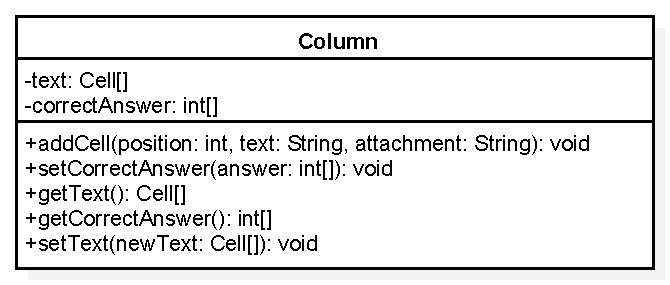
\includegraphics[width=\textwidth]{Img/quizzipedia-client-modelclient-services-questions-column.pdf}}
\caption[Schema Classe Column]{Schema Classe Quizzipedia::Client::ModelClient::Services::Questions::Column}
\end{figure}
\paragraph{Attributi}
\begin{itemize}
\item \attribute{correctAnswer : int[]}
\newline
il corretto ordinamento delle celle della colonna
\item \attribute{text : Cell[]}
\newline
celle che compongono la colonna
\end{itemize}
\paragraph{Metodi}
\begin{itemize}
\item \method{addCell (attachment : String, position : int, text : String) : void}
\newline
permette di aggiungere una nuova cella alla colonna di celle
\newline
\bold{Parametri} :
\begin{itemize}
\item \attribute{attachment : String}
\newline
l'allegato della nuova cella da aggiungere
\item \attribute{position : int}
\newline
la posizione della nuova cella da aggiungere
\item \attribute{text : String}
\newline
il testo della nuova cella da aggiungere
\end{itemize}
\item \method{getCorrectAnswer () : int[]}
\newline
permette di recuperare l'ordine corretto delle celle della colonna
\newline
\item \method{getText () : Cell[]}
\newline
permette di recuperare le celle che compongono la colonna
\newline
\item \method{setCorrectAnswer (answer : int[]) : void}
\newline
permette di aggiornare il corretto ordinamento delle celle
\newline
\bold{Parametri} :
\begin{itemize}
\item \attribute{answer : int[]}
\newline
il corretto ordinamento delle celle della colonna
\end{itemize}
\item \method{setText (newText : Cell[]) : void}
\newline
permette di rimpiazzare completamente tutte le celle con delle celle nuove
\newline
\bold{Parametri} :
\begin{itemize}
\item \attribute{newText : Cell[]}
\newline
le nuove celle che sostituiranno le vecchie nella colonna
\end{itemize}
\end{itemize}
\subsubsection{Classe \cls{CompletionQ}}
Descrive le domande a completamento. Il docente fornirà un testo incompleto e una lista di possibili completamenti; lo studente dovrà inserire le parole adeguate nella giusta posizione.
\begin{figure}[H]
\centering
\noindent\makebox[\textwidth]{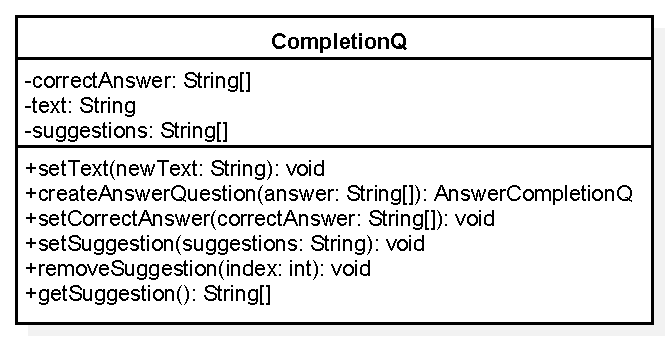
\includegraphics[width=\textwidth]{Img/quizzipedia-client-modelclient-services-questions-completionq.pdf}}
\caption[Schema Classe CompletionQ]{Schema Classe Quizzipedia::Client::ModelClient::Services::Questions::CompletionQ}
\end{figure}
\paragraph{Attributi}
\begin{itemize}
\item \attribute{correctAnswer : String[]}
\newline
le risposte corrette della domanda CompletionQ
\item \attribute{suggestions : String[]}
\newline
i suggerimenti della domanda CompletionQ
\item \attribute{text : String}
\newline
il testo della domanda CompletionQ
\end{itemize}
\paragraph{Metodi}
\begin{itemize}
\item \method{createAnswerQuestion (answer : String[]) : AnswerCompletionQ}
\newline
permette di creare una AnswerCompletionQ che rappresenta una CompletionQ risolta da un utente
\newline
\bold{Parametri} :
\begin{itemize}
\item \attribute{answer : String[]}
\newline
le risposte dell'utente a questa domanda
\end{itemize}
\item \method{getSuggestion () : String[]}
\newline
permette di recuperare i suggerimenti della domanda CompletionQ
\newline
\item \method{removeSuggestion (index : int) : void}
\newline
permette di rimuovere un suggerimento della domanda
\newline
\bold{Parametri} :
\begin{itemize}
\item \attribute{index : int}
\newline
la posizione del suggerimento da rimuovere
\end{itemize}
\item \method{setCorrectAnswer (correctAnswer : String[]) : void}
\newline
permette di aggiornare la risposta corretta della domanda CompletionQ
\newline
\bold{Parametri} :
\begin{itemize}
\item \attribute{correctAnswer : String[]}
\newline
le nuove risposte corrette della domanda
\end{itemize}
\item \method{setSuggestion (suggestions : String[]) : void}
\newline
permette di inserire dei suggerimenti alla domanda CompletionQ
\newline
\bold{Parametri} :
\begin{itemize}
\item \attribute{suggestions : String[]}
\newline
i nuovi suggerimenti della domanda
\end{itemize}
\item \method{setText (newText : String) : void}
\newline
permette di modificare il test della domanda CompletionQ
\newline
\bold{Parametri} :
\begin{itemize}
\item \attribute{newText : String}
\newline
il nuovo testo della domanda
\end{itemize}
\end{itemize}
\subsubsection{Classe \cls{GenericQuestion}}
Descrive le parti comuni a tutti i tipi di domanda presenti nel sistema.
\begin{figure}[H]
\centering
\noindent\makebox[\textwidth]{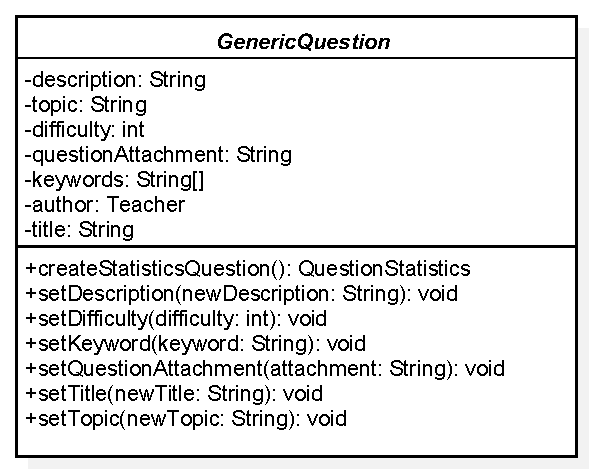
\includegraphics[width=\textwidth]{Img/quizzipedia-client-modelclient-services-questions-genericquestion.pdf}}
\caption[Schema Classe GenericQuestion]{Schema Classe Quizzipedia::Client::ModelClient::Services::Questions::GenericQuestion}
\end{figure}
\paragraph{Attributi}
\begin{itemize}
\item \attribute{author : Teacher}
\newline
l'autore della domanda
\item \attribute{description : String}
\newline
la descrizione della domanda
\item \attribute{difficulty : int}
\newline
la difficoltà della domanda
\item \attribute{keywords : String[]}
\newline
le parole chiave della domanda
\item \attribute{questionAttachment : String}
\newline
l'allegato della domanda
\item \attribute{title : String}
\newline
il titolo della domanda
\item \attribute{topic : String}
\newline
il topic della domanda
\end{itemize}
\paragraph{Metodi}
\begin{itemize}
\item \method{createStatisticsQuestion () : QuestionStatistics}
\newline
permette di creare un QuestionStatistics con le statistiche della domanda
\newline
\item \method{setDescription (newDescription : String) : void}
\newline
permette la modifica della descrizione della domanda
\newline
\bold{Parametri} :
\begin{itemize}
\item \attribute{newDescription : String}
\newline
la nuova descrizione della domanda
\end{itemize}
\item \method{setDifficulty (difficulty : int) : void}
\newline
permette la modifica della difficoltà della domanda
\newline
\bold{Parametri} :
\begin{itemize}
\item \attribute{difficulty : int}
\newline
la nuova difficoltà della domanda
\end{itemize}
\item \method{setKeyword (keyword : String) : void}
\newline
permette di aggiungere una parola chiave alla domanda
\newline
\bold{Parametri} :
\begin{itemize}
\item \attribute{keyword : String}
\newline
la nuova parola chiave della domanda
\end{itemize}
\item \method{setQuestionAttachment (attachment : String) : void}
\newline
permette di aggiungere un allegato alla domanda
\newline
\bold{Parametri} :
\begin{itemize}
\item \attribute{attachment : String}
\newline
il nuovo allegato della domanda
\end{itemize}
\item \method{setTitle (newTitle : String) : void}
\newline
permette di modificare il titolo della domanda
\newline
\bold{Parametri} :
\begin{itemize}
\item \attribute{newTitle : String}
\newline
il nuovo titolo della domanda
\end{itemize}
\item \method{setTopic (newTopic : String) : void}
\newline
permette l'aggiunta di un topic alla domanda
\newline
\bold{Parametri} :
\begin{itemize}
\item \attribute{newTopic : String}
\newline
il nuovo topic della domanda
\end{itemize}
\end{itemize}
\subsubsection{Classe \cls{MatchingQ}}
La struttura descrive le domande a collegamento. L'utente dovrà formare la risposta collegando le entrate da un numero variabile di colonne .
\begin{figure}[H]
\centering
\noindent\makebox[\textwidth]{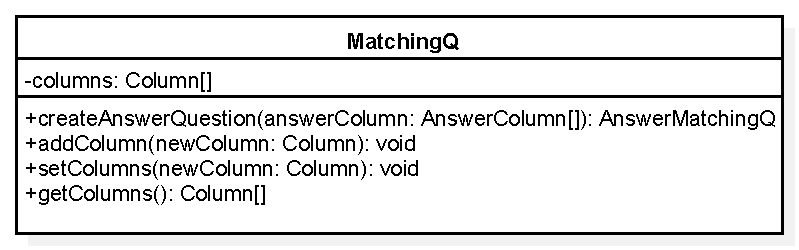
\includegraphics[width=\textwidth]{Img/quizzipedia-client-modelclient-services-questions-matchingq.pdf}}
\caption[Schema Classe MatchingQ]{Schema Classe Quizzipedia::Client::ModelClient::Services::Questions::MatchingQ}
\end{figure}
\paragraph{Attributi}
\begin{itemize}
\item \attribute{column : Column[]}
\newline
le colonne della domanda
\end{itemize}
\paragraph{Metodi}
\begin{itemize}
\item \method{addColumn (newColumn : Column) : void}
\newline
permette di aggiungere una coonna alla domanda MatchingQ
\newline
\bold{Parametri} :
\begin{itemize}
\item \attribute{newColumn : Column}
\newline
la nuova colonna della domanda
\end{itemize}
\item \method{createAnswerQuestion (answerColumn : AnswerColumn[]) : AnswerMatchingQ}
\newline
permette il salvataggio delle risposte dell'utente, sotto forma di AnswerMatchingQ
\newline
\bold{Parametri} :
\begin{itemize}
\item \attribute{answerColumn : AnswerColumn[]}
\newline
le AnswerColumn contenenti le risposte alla domanda
\end{itemize}
\item \method{getColumns () : Column[]}
\newline
permette di ottenere tutte le colonne della domanda
\newline
\item \method{setColumns (newColumn : Column[]) : void}
\newline
permette di sostituire tutte le colonne della domanda MatchingQ con delle nuove colonne
\newline
\bold{Parametri} :
\begin{itemize}
\item \attribute{newColumn : Column[]}
\newline
le nuove colonne della domanda che andranno a sostituire le vecchie
\end{itemize}
\end{itemize}
\subsubsection{Classe \cls{MultipleChoiceQ}}
La struttura descrive le domande a scelta multipla; viene presentata una lista di opzioni tra cui scegliere quelle corrette.
\begin{figure}[H]
\centering
\noindent\makebox[\textwidth]{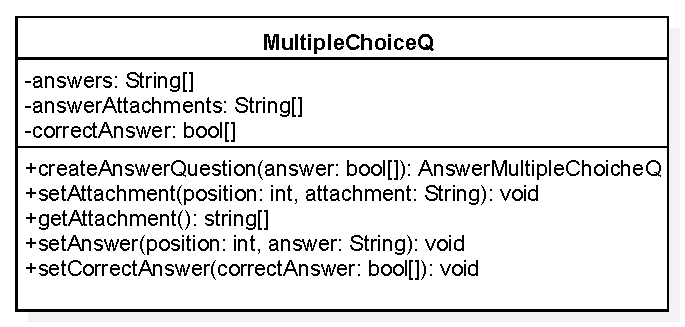
\includegraphics[width=\textwidth]{Img/quizzipedia-client-modelclient-services-questions-multiplechoiceq.pdf}}
\caption[Schema Classe MultipleChoiceQ]{Schema Classe Quizzipedia::Client::ModelClient::Services::Questions::MultipleChoiceQ}
\end{figure}
\paragraph{Attributi}
\begin{itemize}
\item \attribute{answerAttachments : String[]}
\newline
gli allegati delle risposte della domanda
\item \attribute{answers : String[]}
\newline
le risposte della domanda
\item \attribute{correctAnswer : bool[]}
\newline
le soluzione della domanda
\end{itemize}
\paragraph{Metodi}
\begin{itemize}
\item \method{createAnswerQuestion (answer : bool[]) : AnswerMultipleChoicheQ}
\newline
permette di creare un AnswerMultipleChoicheQ con le risposte dell'utente
\newline
\bold{Parametri} :
\begin{itemize}
\item \attribute{answer : bool[]}
\newline
le risposte dell'utente alla domanda
\end{itemize}
\item \method{getAttachment () : String[]}
\newline
permette di recuperare gli allegati della domanda MultipleChoiceQ
\newline
\item \method{setAnswer (answer : String, position : int) : void}
\newline
permette di modificare una risposta corretta della domanda MultipleChoiceQ
\newline
\bold{Parametri} :
\begin{itemize}
\item \attribute{answer : String}
\newline
il testo della risposta
\item \attribute{position : int}
\newline
la posizione della risposta
\end{itemize}
\item \method{setAttachment (attachment : String, position : int) : void}
\newline
permette di aggiungere un allegato alla domanda MultipleChoiceQ
\newline
\bold{Parametri} :
\begin{itemize}
\item \attribute{attachment : String}
\newline
il nuovo allegato
\item \attribute{position : int}
\newline
la posizione del nuovo allegato
\end{itemize}
\item \method{setCorrectAnswer (correctAnswers : bool[]) : void}
\newline
permette di inserire le nuove risposte corrette alla domanda MultipleChoiceQ che sostituiranno le vecchie
\newline
\bold{Parametri} :
\begin{itemize}
\item \attribute{correctAnswers : bool[]}
\newline
le nuove risposte corrette
\end{itemize}
\end{itemize}
\subsubsection{Classe \cls{ShortAnswerQ}}
La struttura descrive le domande aperte, ovvero quelle la cui risposta consiste in un termine o una frase specifici.
\begin{figure}[H]
\centering
\noindent\makebox[\textwidth]{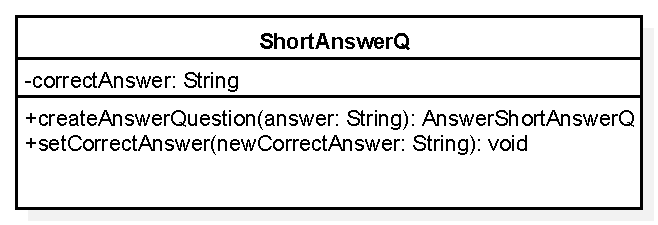
\includegraphics[width=\textwidth]{Img/quizzipedia-client-modelclient-services-questions-shortanswerq.pdf}}
\caption[Schema Classe ShortAnswerQ]{Schema Classe Quizzipedia::Client::ModelClient::Services::Questions::ShortAnswerQ}
\end{figure}
\paragraph{Attributi}
\begin{itemize}
\item \attribute{correctAnswer : String}
\newline
la risposta corretta della domanda ShortAnswerQ
\end{itemize}
\paragraph{Metodi}
\begin{itemize}
\item \method{createAnswerQuestion (answer : String) : AnswerShortAnswerQ}
\newline
permette di creare un AnswerShortAnswerQ con le risposte dell'utente
\newline
\bold{Parametri} :
\begin{itemize}
\item \attribute{answer : String}
\newline
la risposta alla domanda ShortAnswerQ dell'utente
\end{itemize}
\item \method{setCorrectAnswer (newCorrectAnswer : String) : void}
\newline
permette di modificare la risposta corretta della domanda ShortAnswerQ
\newline
\bold{Parametri} :
\begin{itemize}
\item \attribute{newCorrectAnswer : String}
\newline
la nuova risposta corretta della domanda ShortAnswerQ
\end{itemize}
\end{itemize}
\subsubsection{Classe \cls{TrueFalseQ}}
Viene descritta la struttura delle domande che prevedono di decidere la veridicità di un'affermazione.
\begin{figure}[H]
\centering
\noindent\makebox[\textwidth]{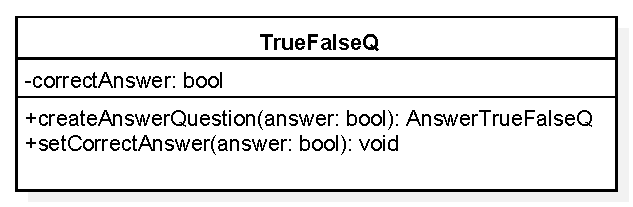
\includegraphics[width=\textwidth]{Img/quizzipedia-client-modelclient-services-questions-truefalseq.pdf}}
\caption[Schema Classe TrueFalseQ]{Schema Classe Quizzipedia::Client::ModelClient::Services::Questions::TrueFalseQ}
\end{figure}
\paragraph{Attributi}
\begin{itemize}
\item \attribute{correctAnswer : bool}
\newline
la risposta corretta alla domanda TrueFalseQ
\end{itemize}
\paragraph{Metodi}
\begin{itemize}
\item \method{createAnswerQuestion (answer : bool) : AnswerTrueFalseQ}
\newline
permette di creare la AnswerTrueFalseQ che contiene la risposta dell'utente
\newline
\bold{Parametri} :
\begin{itemize}
\item \attribute{answer : bool}
\newline
la risposta dell'utente alla domanda TrueFalseQ
\end{itemize}
\item \method{setCorrectAnswer (answer : bool) : void}
\newline
permette di modificare la risposta corretta della domanda TrueFalseQ
\newline
\bold{Parametri} :
\begin{itemize}
\item \attribute{answer : bool}
\newline
la nuova risposta corretta della domanda TrueFalseQ
\end{itemize}
\end{itemize}
\subsection{\pkg{Quizzipedia::Client::ModelClient::Statistics}}
Qui sono raccolte le classi con il compito di reperire informazioni sulle statistiche dal server e presentarle all'utente finale. Sono disponibili statistiche per le domande, per i quiz e per gli studenti di ogni classe.
\begin{figure}[H]
\centering
\noindent\makebox[\textwidth]{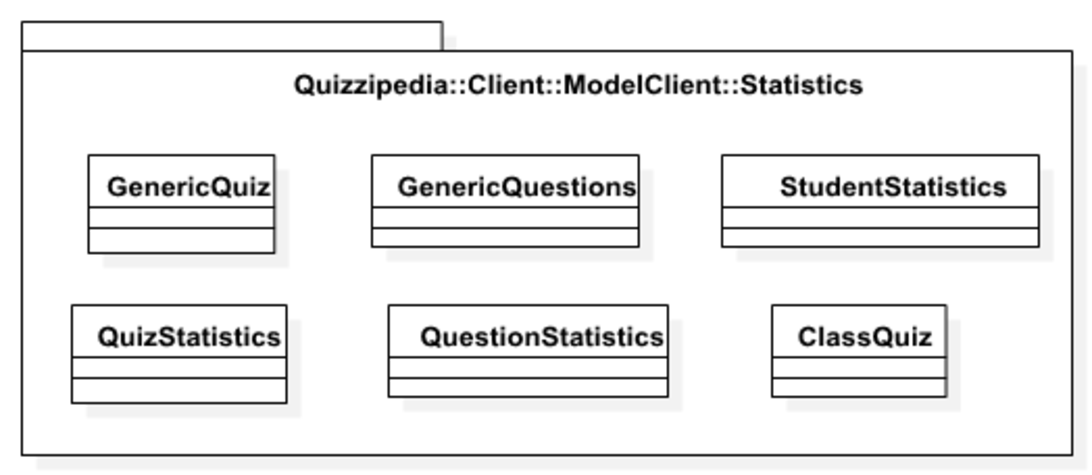
\includegraphics[width=\textwidth]{../SpecificaTecnica/Img/quizzipedia-client-modelclient-statistics.pdf}}
\caption[Schema Componente Quizzipedia::Client::ModelClient::Statistics]{Schema Componente Quizzipedia::Client::ModelClient::Statistics}
\end{figure}
\subsubsection{Classe \cls{QuestionStatistics}}
La classe raccoglie le statistiche principali riguardanti una singola domanda..
\begin{figure}[H]
\centering
\noindent\makebox[\textwidth]{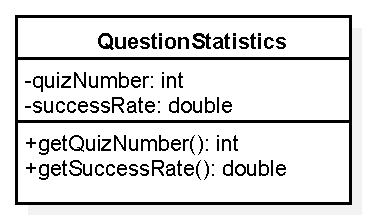
\includegraphics[width=\textwidth]{Img/quizzipedia-client-modelclient-statistics-questionstatistics.pdf}}
\caption[Schema Classe QuestionStatistics]{Schema Classe Quizzipedia::Client::ModelClient::Statistics::QuestionStatistics}
\end{figure}
\paragraph{Attributi}
\begin{itemize}
\item \attribute{quizNumber : int}
\newline
il numero di quiz in cui è presente la domanda
\item \attribute{successRate : double}
\newline
la percentuale di utenti che rispondono correttamente alla domanda
\end{itemize}
\paragraph{Metodi}
\begin{itemize}
\item \method{getQuizNumber () : int}
\newline
restituisce il numero di quiz in cui la domanda è presente
\newline
\item \method{getSuccessRate () : double}
\newline
restituisce la percentuale di utenti che risponde correttamente a questa domanda
\newline
\end{itemize}
\subsubsection{Classe \cls{QuizStatistics}}
La classe raccoglie le statistiche principali riguardanti un singolo quiz.
\begin{figure}[H]
\centering
\noindent\makebox[\textwidth]{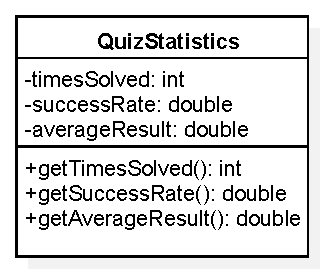
\includegraphics[width=\textwidth]{Img/quizzipedia-client-modelclient-statistics-quizstatistics.pdf}}
\caption[Schema Classe QuizStatistics]{Schema Classe Quizzipedia::Client::ModelClient::Statistics::QuizStatistics}
\end{figure}
\paragraph{Attributi}
\begin{itemize}
\item \attribute{averageResult : double}
\newline
il risultato medio ottenuto da chi ha già risolto il quiz
\item \attribute{successRate : double}
\newline
la percentuale di utenti che ha risolto il quiz con successo
\item \attribute{timesSolved : int}
\newline
il numero di volte che il quiz è stato svolto
\end{itemize}
\paragraph{Metodi}
\begin{itemize}
\item \method{getAverageResult () : double}
\newline
restituisce il risultato medio degli utenti che hanno già svolto il quiz
\newline
\item \method{getSuccessRate () : double}
\newline
restituisce la percentuale di utenti che ha risolto correttamente il quiz
\newline
\item \method{getTimesSolved () : int}
\newline
restituisce il numero di volte che un quiz è stato svolto
\newline
\end{itemize}
\subsubsection{Classe \cls{StudentsStatisticsQuiz}}
Classe usata per visualizzare gli studenti che hanno svolto un quiz specifico e i loro voti per il quiz stesso.
\begin{figure}[H]
\centering
\noindent\makebox[\textwidth]{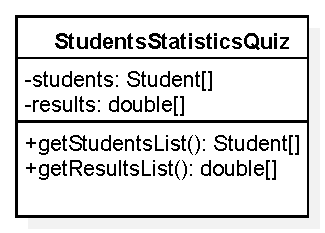
\includegraphics[width=\textwidth]{Img/quizzipedia-client-modelclient-statistics-studentsstatisticsquiz.pdf}}
\caption[Schema Classe StudentsStatisticsQuiz]{Schema Classe Quizzipedia::Client::ModelClient::Statistics::StudentsStatisticsQuiz}
\end{figure}
\paragraph{Attributi}
\begin{itemize}
\item \attribute{results : double[]}
\newline
i risultati ottenuti dagli studenti che hanno risolto il quiz
\item \attribute{students : Student[]}
\newline
gli studenti che hanno svolto il quiz
\end{itemize}
\paragraph{Metodi}
\begin{itemize}
\item \method{getResults () : double[]}
\newline
restituisce la lista dei risultati degli studenti che hanno svolto il quiz
\newline
\item \method{getStudents () : Student[]}
\newline
ottiene la lista degli studenti che hanno svolto il quiz
\newline
\end{itemize}
\subsection{\pkg{Quizzipedia::Client::ModelClient::Users}}
Raccoglie le classi necessarie a descrivere le diverse tipologie di utente che possono accedere al sistema.
\begin{figure}[H]
\centering
\noindent\makebox[\textwidth]{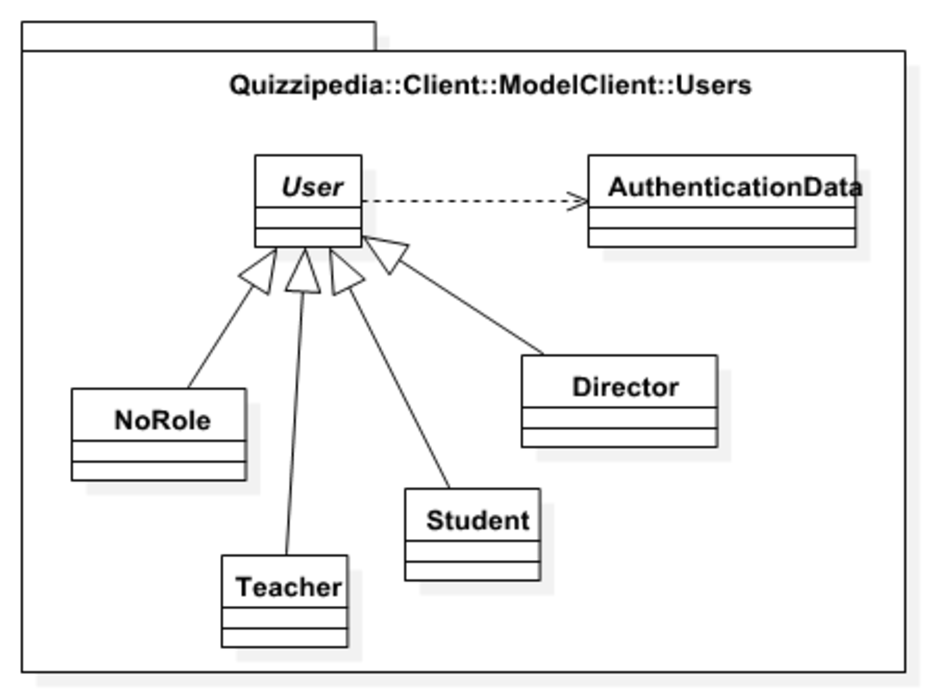
\includegraphics[width=\textwidth]{../SpecificaTecnica/Img/quizzipedia-client-modelclient-users.pdf}}
\caption[Schema Componente Quizzipedia::Client::ModelClient::Users]{Schema Componente Quizzipedia::Client::ModelClient::Users}
\end{figure}
\subsubsection{Classe \cls{AuthenticationData}}
Questa classe gestisce le informazioni di autenticazione comuni a tutti gli utenti.
\begin{figure}[H]
\centering
\noindent\makebox[\textwidth]{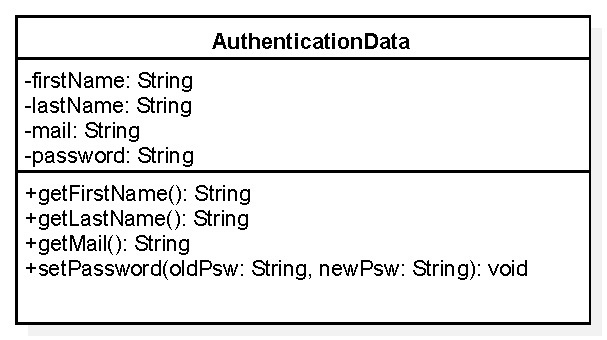
\includegraphics[width=\textwidth]{Img/quizzipedia-client-modelclient-users-authenticationdata.pdf}}
\caption[Schema Classe AuthenticationData]{Schema Classe Quizzipedia::Client::ModelClient::Users::AuthenticationData}
\end{figure}
\paragraph{Attributi}
\begin{itemize}
\item \attribute{firstName : String}
\newline
contiene il nome dell'utente registrato
\item \attribute{lastName : String}
\newline
contiene il cognome dell'utente registrato
\item \attribute{mail : String}
\newline
contiene la mail dell'utente registrato
\item \attribute{password : String}
\newline
contiene la password criptata dell'utente registrato
\end{itemize}
\paragraph{Metodi}
\begin{itemize}
\item \method{getFirstName () : String}
\newline
permette di recuperare il nome dell'utente registrato
\newline
\item \method{getLastName () : String}
\newline
permette di recuperare il cognome dell'utente registrato
\newline
\item \method{getMail () : String}
\newline
permette di recuperare la mail dell'utente registrato
\newline
\item \method{setPassword (newPsw : String, oldPsw : String) : void}
\newline
permette di modificare la password dell'account di un utente registrato
\newline
\bold{Parametri} :
\begin{itemize}
\item \attribute{newPsw : String}
\newline
contiene la nuova password dell'utente
\item \attribute{oldPsw : String}
\newline
contiene la vecchia password dell'utente registrato, necessaria per cambiarla con la nuova
\end{itemize}
\end{itemize}
\subsubsection{Classe \cls{Director}}
Rappresenta un responsabile, ovvero colui che gestisce docenti e studenti per ogni ente del sistema.
\begin{figure}[H]
\centering
\noindent\makebox[\textwidth]{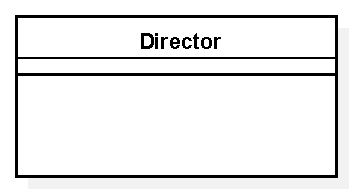
\includegraphics[width=\textwidth]{Img/quizzipedia-client-modelclient-users-director.pdf}}
\caption[Schema Classe Director]{Schema Classe Quizzipedia::Client::ModelClient::Users::Director}
\end{figure}
\paragraph{Metodi}
\begin{itemize}
\item \method{acceptStudent () : void}
\newline
permette di inserire uno studente nell'istituzione posseduta dal direttore
\newline
\item \method{acceptTeacher () : void}
\newline
permette di inserire uno studente nell'istituzione posseduta dal direttore
\newline
\end{itemize}
\subsubsection{Classe \cls{NoRole}}
Rappresenta gli utenti senza ruolo del sistema; coloro che si sono registrati e autenticati ma non hanno ancora fatto richiesta per l'assegnazione ad alcun ruolo.
\begin{figure}[H]
\centering
\noindent\makebox[\textwidth]{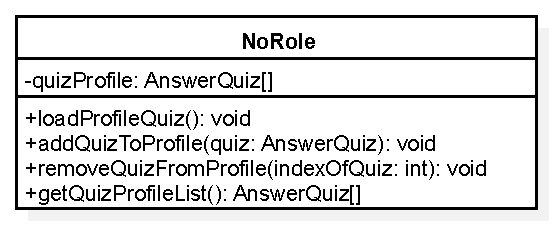
\includegraphics[width=\textwidth]{Img/quizzipedia-client-modelclient-users-norole.pdf}}
\caption[Schema Classe NoRole]{Schema Classe Quizzipedia::Client::ModelClient::Users::NoRole}
\end{figure}
\paragraph{Attributi}
\begin{itemize}
\item \attribute{quizProfile : AnswerQuiz[]}
\newline
è il profilo che raccoglie i quiz già risolti dall'utente e le risposte che l'utente aveva dato
\end{itemize}
\paragraph{Metodi}
\begin{itemize}
\item \method{addQuizToProfile (quiz : AnswerQuiz) : void}
\newline
aggiunge un quiz svolto e le risposte data dall'utente allo storico dei quiz
\newline
\bold{Parametri} :
\begin{itemize}
\item \attribute{quiz : AnswerQuiz}
\newline
la soluzione che si desidera aggiungere alla lista dei quiz già svolti
\end{itemize}
\item \method{getQuizProfile () : AnswerQuiz}
\newline
restituisce la list dei quiz svolti dall'utente e delle relative soluzioni
\newline
\item \method{loadProfileQuiz () : void}
\newline
carica e assegna a quizProfile la lista dei quiz già svolti dall'utente e dei loro esiti
\newline
\item \method{removeQuizFromProfile (indexOfQuiz : int) : void}
\newline
rimuove un quiz e la relativa soluzione dallo storico dei quiz svolti da un utente
\newline
\bold{Parametri} :
\begin{itemize}
\item \attribute{indexOfQuiz : int}
\newline
l'indice del quiz che si desidera rimuovere dallo storico
\end{itemize}
\end{itemize}
\subsubsection{Classe \cls{Student}}
Rappresenta uno studente del sistema e implementa le sue funzioni specifiche oltre a quelle ereditate da utente.
\begin{figure}[H]
\centering
\noindent\makebox[\textwidth]{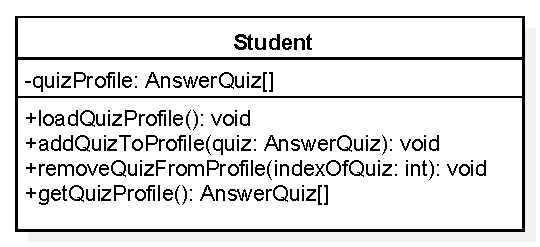
\includegraphics[width=\textwidth]{Img/quizzipedia-client-modelclient-users-student.pdf}}
\caption[Schema Classe Student]{Schema Classe Quizzipedia::Client::ModelClient::Users::Student}
\end{figure}
\paragraph{Attributi}
\begin{itemize}
\item \attribute{quizProfile : AnswerQuiz}
\newline
lo storico dei quiz svolti con relativa soluzione
\end{itemize}
\paragraph{Metodi}
\begin{itemize}
\item \method{addQuizToProfile (quiz : AnswerQuiz) : void}
\newline
aggiunge un quiz e la relativa soluzione allo storico dei quiz svolti
\newline
\bold{Parametri} :
\begin{itemize}
\item \attribute{quiz : AnswerQuiz}
\newline
il quiz che si intende aggiungere allo storico
\end{itemize}
\item \method{getQuizProfile () : AnswerQuiz[]}
\newline
restituisce lo storico dei quiz svolti dall'utente con relative soluzioni
\newline
\item \method{loadQuizProfile () : void}
\newline
carica lo storico dei quiz svolti dall'utente e dei loro esiti
\newline
\item \method{removeQuizFromProfile (indexOfQuiz : int) : void}
\newline
rimuove un quiz e la relativa soluzione dallo storico dei quiz svolti
\newline
\bold{Parametri} :
\begin{itemize}
\item \attribute{indexOfQuiz : int}
\newline
l'indice del quiz che si intende rimuovere dallo storico
\end{itemize}
\end{itemize}
\subsubsection{Classe \cls{Teacher}}
Rappresenta un docente del sistema e ne implementa le funzionalità specifiche in aggiunta a quelle comuni a tutti gli utenti.
\begin{figure}[H]
\centering
\noindent\makebox[\textwidth]{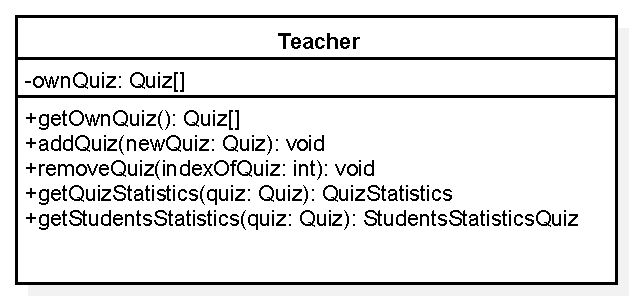
\includegraphics[width=\textwidth]{Img/quizzipedia-client-modelclient-users-teacher.pdf}}
\caption[Schema Classe Teacher]{Schema Classe Quizzipedia::Client::ModelClient::Users::Teacher}
\end{figure}
\paragraph{Attributi}
\begin{itemize}
\item \attribute{ownQuiz : Quiz[]}
\newline
la lista dei quiz creati dall'utente
\end{itemize}
\paragraph{Metodi}
\begin{itemize}
\item \method{addQuiz (newQuiz : Quiz) : void}
\newline
aggiunge un quiz alla lista dei quiz creati dal docente
\newline
\bold{Parametri} :
\begin{itemize}
\item \attribute{newQuiz : Quiz}
\newline
il quiz che si intende aggiungere
\end{itemize}
\item \method{getOwnQuiz () : Quiz[]}
\newline
restituisce la lista dei quiz creati dal docente
\newline
\item \method{getQuizStatistics () : QuizStatistics}
\newline
restituisce le statistiche generali del quiz richiesto
\newline
\item \method{getStudentsStatistics () : StudentsStatisticsQuiz}
\newline
restituisce le statistiche degli utenti che hanno risolto il quiz richiesto
\newline
\item \method{removeQuiz (indexOfQuiz : int) : void}
\newline
rimuove un quiz dalla lista di quiz creati dall'utente
\newline
\bold{Parametri} :
\begin{itemize}
\item \attribute{indexOfQuiz : int}
\newline
l'indice del quiz che si intende rimuovere
\end{itemize}
\end{itemize}
\subsubsection{Classe \cls{User}}
Questa è una classe astratta e raccoglie le funzionalità comuni a tutti gli utenti.
\begin{figure}[H]
\centering
\noindent\makebox[\textwidth]{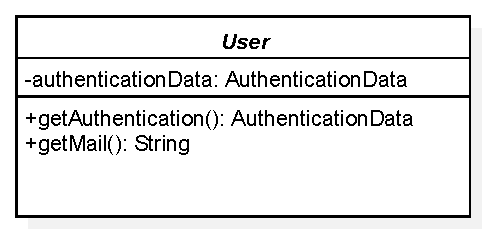
\includegraphics[width=\textwidth]{Img/quizzipedia-client-modelclient-users-user.pdf}}
\caption[Schema Classe User]{Schema Classe Quizzipedia::Client::ModelClient::Users::User}
\end{figure}
\paragraph{Attributi}
\begin{itemize}
\item \attribute{authenticationData : AuthenticationData}
\newline
raccoglie le informazioni di base dell'utente, necessarie alla sua autenticazione. Sono comuni in tutta la gerarchia
\end{itemize}
\paragraph{Metodi}
\begin{itemize}
\item \method{getAuthenticationData () : AuthenticationData}
\newline
restituisce i dati necessari all'autenticazione dell'utente
\newline
\item \method{getMail () : String}
\newline
restituisce la mail dell'utente, che è univoca
\newline
\end{itemize}
\subsection{\pkg{Quizzipedia::Client::ViewClient}}
Racchiude tutte le componenti necessarie per presentare il prodotto all'utente.
Grazie all'uso di Angular.js ogni modifica svolta dall'utente si ripercuoterà automaticamente a sulla componente model, attraverso il controller, per mantenere sempre le informazioni consistenti e aggiornate.
Con l'uso invece di Bootstrap e Fabric.js a livello di grafica web risulta semplificata l'impaginazione delle singole pagine web dedicate all'utente e alla gestione di allegati non testuali all'interno di domande.
\begin{figure}[H]
\centering
\noindent\makebox[\textwidth]{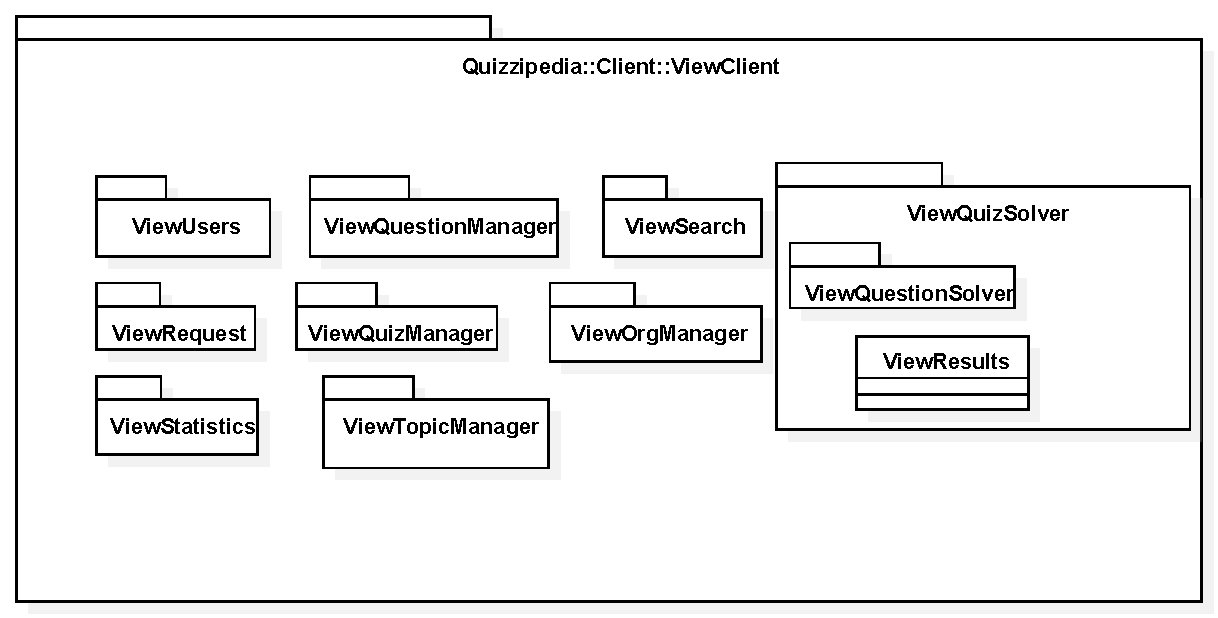
\includegraphics[width=\textwidth]{../SpecificaTecnica/Img/quizzipedia-client-viewclient.pdf}}
\caption[Schema Componente Quizzipedia::Client::ViewClient]{Schema Componente Quizzipedia::Client::ViewClient}
\end{figure}
\subsection{\pkg{Quizzipedia::Client::ViewClient::Shared}}
Contiene componenti condivise da più pagine del sistema, che vengono quindi qui raccolte perché siano accessibili a tutti.
\begin{figure}[H]
\centering
\noindent\makebox[\textwidth]{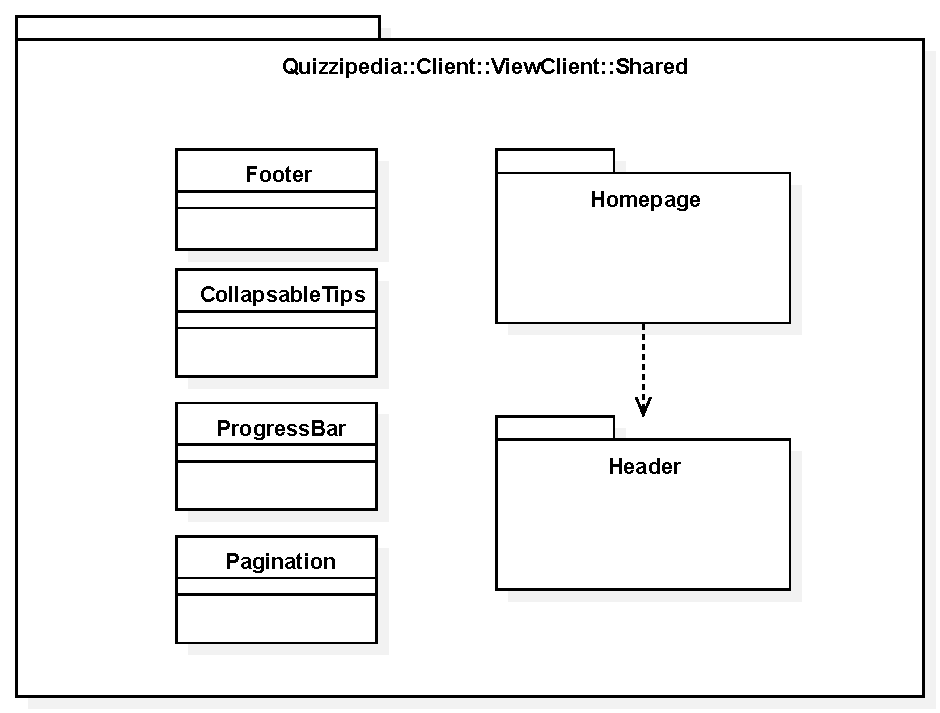
\includegraphics[width=\textwidth]{../SpecificaTecnica/Img/quizzipedia-client-viewclient-shared.pdf}}
\caption[Schema Componente Quizzipedia::Client::ViewClient::Shared]{Schema Componente Quizzipedia::Client::ViewClient::Shared}
\end{figure}
\subsubsection{Classe \cls{CollapsableTips}}
Contiene il codice necessario a creare il dato elemento grafico.
\begin{figure}[H]
\centering
\noindent\makebox[\textwidth]{\includegraphics[width=\textwidth]{Img/quizzipedia-client-viewclient-shared-collapsabletips.pdf}}
\caption[Schema Classe CollapsableTips]{Schema Classe Quizzipedia::Client::ViewClient::Shared::CollapsableTips}
\end{figure}
\subsubsection{Classe \cls{Footer}}
Contiene il codice necessario a creare il footer, che è costante su tutte le pagine del sito.
\begin{figure}[H]
\centering
\noindent\makebox[\textwidth]{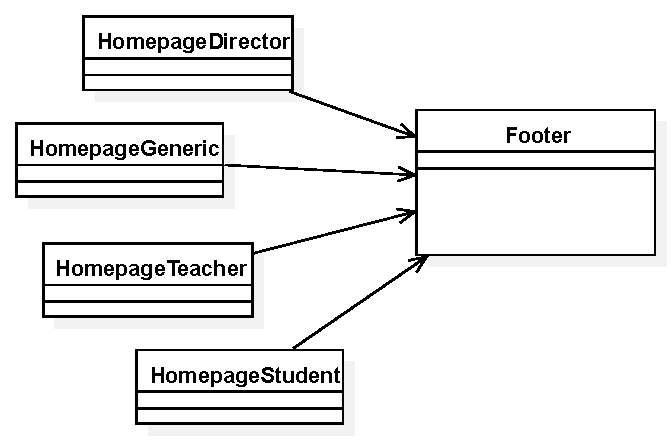
\includegraphics[width=\textwidth]{Img/quizzipedia-client-viewclient-shared-footer.pdf}}
\caption[Schema Classe Footer]{Schema Classe Quizzipedia::Client::ViewClient::Shared::Footer}
\end{figure}
\subsubsection{Classe \cls{Pagination}}
Contiene il codice necessario a gestire il sistema di paginazione.
\begin{figure}[H]
\centering
\noindent\makebox[\textwidth]{\includegraphics[width=\textwidth]{Img/quizzipedia-client-viewclient-shared-pagination.pdf}}
\caption[Schema Classe Pagination]{Schema Classe Quizzipedia::Client::ViewClient::Shared::Pagination}
\end{figure}
\subsubsection{Classe \cls{ProgressBar}}
Contiene il codice necessario a creare la barra di progresso.
\begin{figure}[H]
\centering
\noindent\makebox[\textwidth]{\includegraphics[width=\textwidth]{Img/quizzipedia-client-viewclient-shared-progressbar.pdf}}
\caption[Schema Classe ProgressBar]{Schema Classe Quizzipedia::Client::ViewClient::Shared::ProgressBar}
\end{figure}
\subsection{\pkg{Quizzipedia::Client::ViewClient::Shared::Header}}
Contiene i template per caricare header e breadcrumb delle pagine a seconda della posizione e del ruolo dell'utente.
\begin{figure}[H]
\centering
\noindent\makebox[\textwidth]{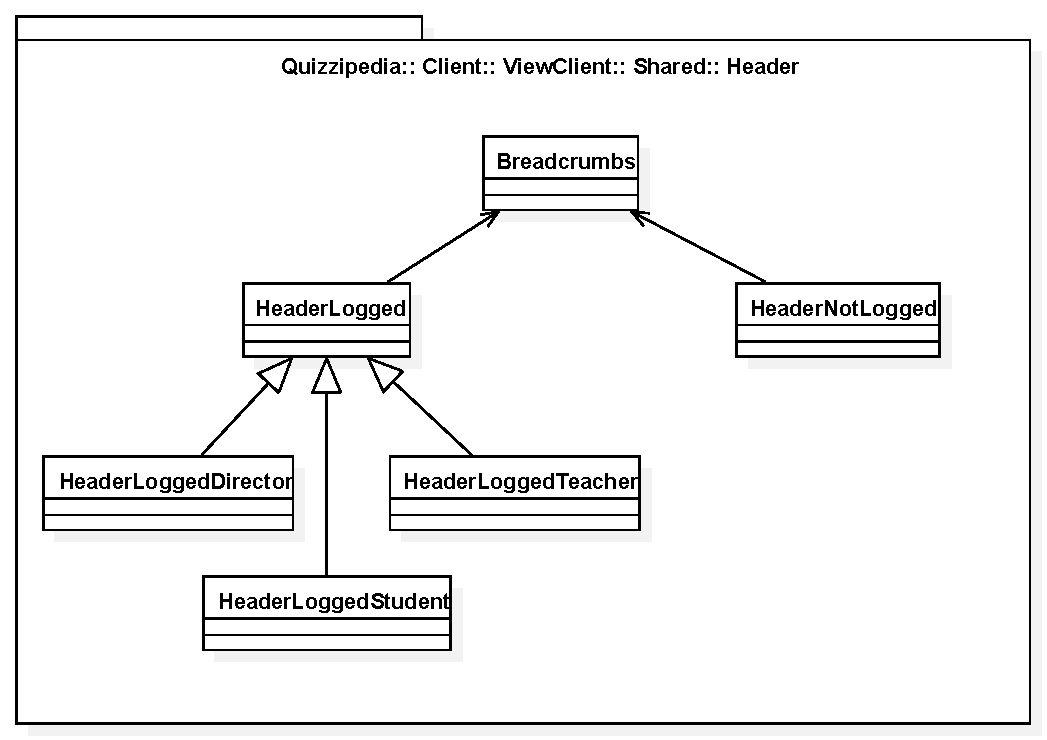
\includegraphics[width=\textwidth]{../SpecificaTecnica/Img/quizzipedia-client-viewclient-shared-header.pdf}}
\caption[Schema Componente Quizzipedia::Client::ViewClient::Shared::Header]{Schema Componente Quizzipedia::Client::ViewClient::Shared::Header}
\end{figure}
\subsubsection{Classe \cls{Breadcrumbs}}
Contiene il codice necessario a creare il breadcrumb.
\begin{figure}[H]
\centering
\noindent\makebox[\textwidth]{\includegraphics[width=\textwidth]{Img/quizzipedia-client-viewclient-shared-header-breadcrumbs.pdf}}
\caption[Schema Classe Breadcrumbs]{Schema Classe Quizzipedia::Client::ViewClient::Shared::Header::Breadcrumbs}
\end{figure}
\subsubsection{Classe \cls{HeaderLogged}}
Carica lo header che verrà visualizzato dall'utente registrato.
\begin{figure}[H]
\centering
\noindent\makebox[\textwidth]{\includegraphics[width=\textwidth]{Img/quizzipedia-client-viewclient-shared-header-headerlogged.pdf}}
\caption[Schema Classe HeaderLogged]{Schema Classe Quizzipedia::Client::ViewClient::Shared::Header::HeaderLogged}
\end{figure}
\subsubsection{Classe \cls{HeaderLoggedDirector}}
Carica lo header che verrà visualizzato dal responsabile.
\begin{figure}[H]
\centering
\noindent\makebox[\textwidth]{\includegraphics[width=\textwidth]{Img/quizzipedia-client-viewclient-shared-header-headerloggeddirector.pdf}}
\caption[Schema Classe HeaderLoggedDirector]{Schema Classe Quizzipedia::Client::ViewClient::Shared::Header::HeaderLoggedDirector}
\end{figure}
\subsubsection{Classe \cls{HeaderLoggedStudent}}
Carica lo header che verrà visualizzato dallo studente.
\begin{figure}[H]
\centering
\noindent\makebox[\textwidth]{\includegraphics[width=\textwidth]{Img/quizzipedia-client-viewclient-shared-header-headerloggedstudent.pdf}}
\caption[Schema Classe HeaderLoggedStudent]{Schema Classe Quizzipedia::Client::ViewClient::Shared::Header::HeaderLoggedStudent}
\end{figure}
\subsubsection{Classe \cls{HeaderLoggedTeacher}}
Carica lo header che verrà visualizzato dall'insegnante.
\begin{figure}[H]
\centering
\noindent\makebox[\textwidth]{\includegraphics[width=\textwidth]{Img/quizzipedia-client-viewclient-shared-header-headerloggedteacher.pdf}}
\caption[Schema Classe HeaderLoggedTeacher]{Schema Classe Quizzipedia::Client::ViewClient::Shared::Header::HeaderLoggedTeacher}
\end{figure}
\subsubsection{Classe \cls{HeaderNotLogged}}
Carica lo header che verrà visualizzato da un visitatore non registrato.
\begin{figure}[H]
\centering
\noindent\makebox[\textwidth]{\includegraphics[width=\textwidth]{Img/quizzipedia-client-viewclient-shared-header-headernotlogged.pdf}}
\caption[Schema Classe HeaderNotLogged]{Schema Classe Quizzipedia::Client::ViewClient::Shared::Header::HeaderNotLogged}
\end{figure}
\subsection{\pkg{Quizzipedia::Client::ViewClient::Shared::Homepage}}
Contiene le pagine necessarie alla creazione della homepage e delle parti che possono variare a seconda del tipo di utente che la visita.
\begin{figure}[H]
\centering
\noindent\makebox[\textwidth]{\includegraphics[width=\textwidth]{../SpecificaTecnica/Img/quizzipedia-client-viewclient-shared-homepage.pdf}}
\caption[Schema Componente Quizzipedia::Client::ViewClient::Shared::Homepage]{Schema Componente Quizzipedia::Client::ViewClient::Shared::Homepage}
\end{figure}
\subsubsection{Classe \cls{HomepageDirector}}
Carica la homepage che verrà visualizzata dal responsabile.
\begin{figure}[H]
\centering
\noindent\makebox[\textwidth]{\includegraphics[width=\textwidth]{Img/quizzipedia-client-viewclient-shared-homepage-homepagedirector.pdf}}
\caption[Schema Classe HomepageDirector]{Schema Classe Quizzipedia::Client::ViewClient::Shared::Homepage::HomepageDirector}
\end{figure}
\subsubsection{Classe \cls{HomepageGeneric}}
Carica la homepage che verrà visualizzata da un visitatore generico.
\begin{figure}[H]
\centering
\noindent\makebox[\textwidth]{\includegraphics[width=\textwidth]{Img/quizzipedia-client-viewclient-shared-homepage-homepagegeneric.pdf}}
\caption[Schema Classe HomepageGeneric]{Schema Classe Quizzipedia::Client::ViewClient::Shared::Homepage::HomepageGeneric}
\end{figure}
\subsubsection{Classe \cls{HomepageStudent}}
Carica la homepage che verrà visualizzata dallo studente.
\begin{figure}[H]
\centering
\noindent\makebox[\textwidth]{\includegraphics[width=\textwidth]{Img/quizzipedia-client-viewclient-shared-homepage-homepagestudent.pdf}}
\caption[Schema Classe HomepageStudent]{Schema Classe Quizzipedia::Client::ViewClient::Shared::Homepage::HomepageStudent}
\end{figure}
\subsubsection{Classe \cls{HomepageTeacher}}
Carica la homepage che verrà visualizzata dal docente.
\begin{figure}[H]
\centering
\noindent\makebox[\textwidth]{\includegraphics[width=\textwidth]{Img/quizzipedia-client-viewclient-shared-homepage-homepageteacher.pdf}}
\caption[Schema Classe HomepageTeacher]{Schema Classe Quizzipedia::Client::ViewClient::Shared::Homepage::HomepageTeacher}
\end{figure}
\subsection{\pkg{Quizzipedia::Client::ViewClient::ViewOrgManager}}
Qui sono raccolte le classi responsabili della presentazione delle pagine da cui sarà possibile gestire le classi e gli enti presenti in Quizzipedia.
\begin{figure}[H]
\centering
\noindent\makebox[\textwidth]{\includegraphics[width=\textwidth]{../SpecificaTecnica/Img/quizzipedia-client-viewclient-vieworgmanager.pdf}}
\caption[Schema Componente Quizzipedia::Client::ViewClient::ViewOrgManager]{Schema Componente Quizzipedia::Client::ViewClient::ViewOrgManager}
\end{figure}
\subsubsection{Classe \cls{ViewClassMembers}}
La classe si occupa di presentare una lista degli utenti iscritti alla classe e altre informazioni aggiuntive.
\begin{figure}[H]
\centering
\noindent\makebox[\textwidth]{\includegraphics[width=\textwidth]{Img/quizzipedia-client-viewclient-vieworgmanager-viewclassmembers.pdf}}
\caption[Schema Classe ViewClassMembers]{Schema Classe Quizzipedia::Client::ViewClient::ViewOrgManager::ViewClassMembers}
\end{figure}
\subsubsection{Classe \cls{ViewModifyOrg}}
Presenta all'utente la pagina da cui sarà possibile modificare le informazioni su una classe o su un ente esistente.
\begin{figure}[H]
\centering
\noindent\makebox[\textwidth]{\includegraphics[width=\textwidth]{Img/quizzipedia-client-viewclient-vieworgmanager-viewmodifyorg.pdf}}
\caption[Schema Classe ViewModifyOrg]{Schema Classe Quizzipedia::Client::ViewClient::ViewOrgManager::ViewModifyOrg}
\end{figure}
\subsection{\pkg{Quizzipedia::Client::ViewClient::ViewQuestionManager}}
Qui sono raccolte le classi responsabili della presentazione delle pagine da cui sarà possibile gestire le domande.
\begin{figure}[H]
\centering
\noindent\makebox[\textwidth]{\includegraphics[width=\textwidth]{../SpecificaTecnica/Img/quizzipedia-client-viewclient-viewquestionmanager.pdf}}
\caption[Schema Componente Quizzipedia::Client::ViewClient::ViewQuestionManager]{Schema Componente Quizzipedia::Client::ViewClient::ViewQuestionManager}
\end{figure}
\subsubsection{Classe \cls{CreateCompletionQ}}
Presenta la pagina da cui sarà possibile creare una nuova domanda a completamento.
\begin{figure}[H]
\centering
\noindent\makebox[\textwidth]{\includegraphics[width=\textwidth]{Img/quizzipedia-client-viewclient-viewquestionmanager-createcompletionq.pdf}}
\caption[Schema Classe CreateCompletionQ]{Schema Classe Quizzipedia::Client::ViewClient::ViewQuestionManager::CreateCompletionQ}
\end{figure}
\subsubsection{Classe \cls{CreateGenericQ}}
Presenta la pagina da cui è possibile creare una nuova domanda, inserendo le informazioni comuni a tutte le domande. Poi si potrà selezionare il tipo di domanda desiderato.
\begin{figure}[H]
\centering
\noindent\makebox[\textwidth]{\includegraphics[width=\textwidth]{Img/quizzipedia-client-viewclient-viewquestionmanager-creategenericq.pdf}}
\caption[Schema Classe CreateGenericQ]{Schema Classe Quizzipedia::Client::ViewClient::ViewQuestionManager::CreateGenericQ}
\end{figure}
\subsubsection{Classe \cls{CreateMatchingQ}}
Presenta la pagina da cui sarà possibile creare una nuova domanda a collegamenti.
\begin{figure}[H]
\centering
\noindent\makebox[\textwidth]{\includegraphics[width=\textwidth]{Img/quizzipedia-client-viewclient-viewquestionmanager-creatematchingq.pdf}}
\caption[Schema Classe CreateMatchingQ]{Schema Classe Quizzipedia::Client::ViewClient::ViewQuestionManager::CreateMatchingQ}
\end{figure}
\subsubsection{Classe \cls{CreateMultipleChoiceQ}}
Presenta la pagina da cui sarà possibile creare una nuova domanda a scelta multipla.
\begin{figure}[H]
\centering
\noindent\makebox[\textwidth]{\includegraphics[width=\textwidth]{Img/quizzipedia-client-viewclient-viewquestionmanager-createmultiplechoiceq.pdf}}
\caption[Schema Classe CreateMultipleChoiceQ]{Schema Classe Quizzipedia::Client::ViewClient::ViewQuestionManager::CreateMultipleChoiceQ}
\end{figure}
\subsubsection{Classe \cls{CreateShortAnswerQ}}
Presenta la pagina da cui sarà possibile creare una nuova domanda aperta.
\begin{figure}[H]
\centering
\noindent\makebox[\textwidth]{\includegraphics[width=\textwidth]{Img/quizzipedia-client-viewclient-viewquestionmanager-createshortanswerq.pdf}}
\caption[Schema Classe CreateShortAnswerQ]{Schema Classe Quizzipedia::Client::ViewClient::ViewQuestionManager::CreateShortAnswerQ}
\end{figure}
\subsubsection{Classe \cls{CreateTrueFalseQ}}
Presenta la pagina da cui sarà possibile creare una nuova domanda di tipo vero/falso.
\begin{figure}[H]
\centering
\noindent\makebox[\textwidth]{\includegraphics[width=\textwidth]{Img/quizzipedia-client-viewclient-viewquestionmanager-createtruefalseq.pdf}}
\caption[Schema Classe CreateTrueFalseQ]{Schema Classe Quizzipedia::Client::ViewClient::ViewQuestionManager::CreateTrueFalseQ}
\end{figure}
\subsubsection{Classe \cls{QuestionMgmt}}
Presenta all'utente il pannello da cui sarà possibile creare una nuova domanda e visualizzare una lista di informazioni riassuntive sulle domande già create, con possibilità di modifica e rimozione.
\begin{figure}[H]
\centering
\noindent\makebox[\textwidth]{\includegraphics[width=\textwidth]{Img/quizzipedia-client-viewclient-viewquestionmanager-questionmgmt.pdf}}
\caption[Schema Classe QuestionMgmt]{Schema Classe Quizzipedia::Client::ViewClient::ViewQuestionManager::QuestionMgmt}
\end{figure}
\subsection{\pkg{Quizzipedia::Client::ViewClient::ViewQuizManager}}
Qui sono raccolte le classi responsabili della presentazione delle pagine da cui sarà possibile gestire i quiz.
\begin{figure}[H]
\centering
\noindent\makebox[\textwidth]{\includegraphics[width=\textwidth]{../SpecificaTecnica/Img/quizzipedia-client-viewclient-viewquizmanager.pdf}}
\caption[Schema Componente Quizzipedia::Client::ViewClient::ViewQuizManager]{Schema Componente Quizzipedia::Client::ViewClient::ViewQuizManager}
\end{figure}
\subsubsection{Classe \cls{ViewCreateQuiz}}
Presenta la pagina da cui sarà possibile creare un nuovo quiz.
\begin{figure}[H]
\centering
\noindent\makebox[\textwidth]{\includegraphics[width=\textwidth]{Img/quizzipedia-client-viewclient-viewquizmanager-viewcreatequiz.pdf}}
\caption[Schema Classe ViewCreateQuiz]{Schema Classe Quizzipedia::Client::ViewClient::ViewQuizManager::ViewCreateQuiz}
\end{figure}
\subsubsection{Classe \cls{ViewEditQuiz}}
Presenta all'utente una pagina da cui è possibile modificare nel dettaglio un quiz esistente, intervenendo sulle domande che lo compongono.
\begin{figure}[H]
\centering
\noindent\makebox[\textwidth]{\includegraphics[width=\textwidth]{Img/quizzipedia-client-viewclient-viewquizmanager-vieweditquiz.pdf}}
\caption[Schema Classe ViewEditQuiz]{Schema Classe Quizzipedia::Client::ViewClient::ViewQuizManager::ViewEditQuiz}
\end{figure}
\subsubsection{Classe \cls{ViewQuizMgmt}}
Carica una pagina contenente una lista con informazioni riassuntive sui quiz e un pannello da cui sarà possibile svolgere operazioni di modifica e rimozione. Da qui è inoltre possibile creare nuovi quiz.
\begin{figure}[H]
\centering
\noindent\makebox[\textwidth]{\includegraphics[width=\textwidth]{Img/quizzipedia-client-viewclient-viewquizmanager-viewquizmgmt.pdf}}
\caption[Schema Classe ViewQuizMgmt]{Schema Classe Quizzipedia::Client::ViewClient::ViewQuizManager::ViewQuizMgmt}
\end{figure}
\subsection{\pkg{Quizzipedia::Client::ViewClient::ViewQuizSolver}}
Il componente raccoglie le classi necessarie alla visualizzazione delle pagine da cui sarà possibile svolgere quiz.
\begin{figure}[H]
\centering
\noindent\makebox[\textwidth]{\includegraphics[width=\textwidth]{../SpecificaTecnica/Img/quizzipedia-client-viewclient-viewquizsolver.pdf}}
\caption[Schema Componente Quizzipedia::Client::ViewClient::ViewQuizSolver]{Schema Componente Quizzipedia::Client::ViewClient::ViewQuizSolver}
\end{figure}
\subsubsection{Classe \cls{ViewQuizExec}}
Pagina da cui sarà possibile svolgere un quiz. Verranno caricate le domande che lo compongono fino al risultato finale.
\begin{figure}[H]
\centering
\noindent\makebox[\textwidth]{\includegraphics[width=\textwidth]{Img/quizzipedia-client-viewclient-viewquizsolver-viewquizexec.pdf}}
\caption[Schema Classe ViewQuizExec]{Schema Classe Quizzipedia::Client::ViewClient::ViewQuizSolver::ViewQuizExec}
\end{figure}
\subsection{\pkg{Quizzipedia::Client::ViewClient::ViewQuizSolver::ViewQuestionSolver}}
Il componente raccoglie le classi necessarie alla visualizzazione delle pagine da cui sarà possibile rispondere alle singole domande.
\begin{figure}[H]
\centering
\noindent\makebox[\textwidth]{\includegraphics[width=\textwidth]{../SpecificaTecnica/Img/quizzipedia-client-viewclient-viewquizsolver-viewquestionsolver.pdf}}
\caption[Schema Componente Quizzipedia::Client::ViewClient::ViewQuizSolver::ViewQuestionSolver]{Schema Componente Quizzipedia::Client::ViewClient::ViewQuizSolver::ViewQuestionSolver}
\end{figure}
\subsubsection{Classe \cls{ViewCompletionQ}}
Presenta all'utente la pagina da cui sarà possibile rispondere a una domanda a completamento.
\begin{figure}[H]
\centering
\noindent\makebox[\textwidth]{\includegraphics[width=\textwidth]{Img/quizzipedia-client-viewclient-viewquizsolver-viewquestionsolver-viewcompletionq.pdf}}
\caption[Schema Classe ViewCompletionQ]{Schema Classe Quizzipedia::Client::ViewClient::ViewQuizSolver::ViewQuestionSolver::ViewCompletionQ}
\end{figure}
\subsubsection{Classe \cls{ViewMatchingQ}}
Presenta all'utente la pagina da cui sarà possibile rispondere a una domanda a collegamenti.
\begin{figure}[H]
\centering
\noindent\makebox[\textwidth]{\includegraphics[width=\textwidth]{Img/quizzipedia-client-viewclient-viewquizsolver-viewquestionsolver-viewmatchingq.pdf}}
\caption[Schema Classe ViewMatchingQ]{Schema Classe Quizzipedia::Client::ViewClient::ViewQuizSolver::ViewQuestionSolver::ViewMatchingQ}
\end{figure}
\subsubsection{Classe \cls{ViewMultipleChoiceQ}}
Presenta all'utente la pagina da cui sarà possibile rispondere a una domanda a risposta multipla.
\begin{figure}[H]
\centering
\noindent\makebox[\textwidth]{\includegraphics[width=\textwidth]{Img/quizzipedia-client-viewclient-viewquizsolver-viewquestionsolver-viewmultiplechoiceq.pdf}}
\caption[Schema Classe ViewMultipleChoiceQ]{Schema Classe Quizzipedia::Client::ViewClient::ViewQuizSolver::ViewQuestionSolver::ViewMultipleChoiceQ}
\end{figure}
\subsubsection{Classe \cls{ViewShortAnswerQ}}
Presenta all'utente la pagina da cui sarà possibile rispondere a una domanda a risposta aperta.
\begin{figure}[H]
\centering
\noindent\makebox[\textwidth]{\includegraphics[width=\textwidth]{Img/quizzipedia-client-viewclient-viewquizsolver-viewquestionsolver-viewshortanswerq.pdf}}
\caption[Schema Classe ViewShortAnswerQ]{Schema Classe Quizzipedia::Client::ViewClient::ViewQuizSolver::ViewQuestionSolver::ViewShortAnswerQ}
\end{figure}
\subsubsection{Classe \cls{ViewTrueFalseQ}}
Presenta all'utente la pagina da cui sarà possibile rispondere a una domanda di tipo vero/falso.
\begin{figure}[H]
\centering
\noindent\makebox[\textwidth]{\includegraphics[width=\textwidth]{Img/quizzipedia-client-viewclient-viewquizsolver-viewquestionsolver-viewtruefalseq.pdf}}
\caption[Schema Classe ViewTrueFalseQ]{Schema Classe Quizzipedia::Client::ViewClient::ViewQuizSolver::ViewQuestionSolver::ViewTrueFalseQ}
\end{figure}
\subsection{\pkg{Quizzipedia::Client::ViewClient::ViewRequests}}
Qui sono raccolte le pagine che permettono all'utente di inviare e gestire le richieste di ruolo e classe.
\begin{figure}[H]
\centering
\noindent\makebox[\textwidth]{\includegraphics[width=\textwidth]{../SpecificaTecnica/Img/quizzipedia-client-viewclient-viewrequests.pdf}}
\caption[Schema Componente Quizzipedia::Client::ViewClient::ViewRequests]{Schema Componente Quizzipedia::Client::ViewClient::ViewRequests}
\end{figure}
\subsubsection{Classe \cls{SendRequests}}
È la pagina da cui l'utente potrà richiedere di entrare in una classe o che gli venga assegnato un ruolo in un ente.
\begin{figure}[H]
\centering
\noindent\makebox[\textwidth]{\includegraphics[width=\textwidth]{Img/quizzipedia-client-viewclient-viewrequests-sendrequests.pdf}}
\caption[Schema Classe SendRequests]{Schema Classe Quizzipedia::Client::ViewClient::ViewRequests::SendRequests}
\end{figure}
\subsubsection{Classe \cls{ViewPendingRequests}}
Visualizza il pannello da cui sarà possibile gestire le richieste di inserimento in una classe e le richieste di assegnazione di ruolo pendenti.
\begin{figure}[H]
\centering
\noindent\makebox[\textwidth]{\includegraphics[width=\textwidth]{Img/quizzipedia-client-viewclient-viewrequests-viewpendingrequests.pdf}}
\caption[Schema Classe ViewPendingRequests]{Schema Classe Quizzipedia::Client::ViewClient::ViewRequests::ViewPendingRequests}
\end{figure}
\subsection{\pkg{Quizzipedia::Client::ViewClient::ViewSearch}}
Il componente contiene le classi responsabili della creazione delle pagine da cui sarà possibile ricercare domande, quiz, istituti e classi all'interno degli enti.
\begin{figure}[H]
\centering
\noindent\makebox[\textwidth]{\includegraphics[width=\textwidth]{../SpecificaTecnica/Img/quizzipedia-client-viewclient-viewsearch.pdf}}
\caption[Schema Componente Quizzipedia::Client::ViewClient::ViewSearch]{Schema Componente Quizzipedia::Client::ViewClient::ViewSearch}
\end{figure}
\subsubsection{Classe \cls{ViewSearchClass}}
La classe carica la pagina da cui sarà possibile ricercare enti e classi all'interno di un ente.
\begin{figure}[H]
\centering
\noindent\makebox[\textwidth]{\includegraphics[width=\textwidth]{Img/quizzipedia-client-viewclient-viewsearch-viewsearchclass.pdf}}
\caption[Schema Classe ViewSearchClass]{Schema Classe Quizzipedia::Client::ViewClient::ViewSearch::ViewSearchClass}
\end{figure}
\subsubsection{Classe \cls{ViewSearchQuestions}}
Classe che ha il compito di caricare la pagina da cui sarà possibile effettuare la ricerca di domande.
\begin{figure}[H]
\centering
\noindent\makebox[\textwidth]{\includegraphics[width=\textwidth]{Img/quizzipedia-client-viewclient-viewsearch-viewsearchquestions.pdf}}
\caption[Schema Classe ViewSearchQuestions]{Schema Classe Quizzipedia::Client::ViewClient::ViewSearch::ViewSearchQuestions}
\end{figure}
\subsubsection{Classe \cls{ViewSearchQuiz}}
Raccoglie i metodi necessari alla creazione della pagina da cui sarà possibile cercare un quiz.
\begin{figure}[H]
\centering
\noindent\makebox[\textwidth]{\includegraphics[width=\textwidth]{Img/quizzipedia-client-viewclient-viewsearch-viewsearchquiz.pdf}}
\caption[Schema Classe ViewSearchQuiz]{Schema Classe Quizzipedia::Client::ViewClient::ViewSearch::ViewSearchQuiz}
\end{figure}
\subsection{\pkg{Quizzipedia::Client::ViewClient::ViewStatistics}}
Componente che gestisce le pagine in cui verranno visualizzate le statistiche richieste dall'utente.
\begin{figure}[H]
\centering
\noindent\makebox[\textwidth]{\includegraphics[width=\textwidth]{../SpecificaTecnica/Img/quizzipedia-client-viewclient-viewstatistics.pdf}}
\caption[Schema Componente Quizzipedia::Client::ViewClient::ViewStatistics]{Schema Componente Quizzipedia::Client::ViewClient::ViewStatistics}
\end{figure}
\subsubsection{Classe \cls{ViewQuestionStats}}
Vengono rappresentate le statistiche generali relative alle domande.
\begin{figure}[H]
\centering
\noindent\makebox[\textwidth]{\includegraphics[width=\textwidth]{Img/quizzipedia-client-viewclient-viewstatistics-viewquestionstats.pdf}}
\caption[Schema Classe ViewQuestionStats]{Schema Classe Quizzipedia::Client::ViewClient::ViewStatistics::ViewQuestionStats}
\end{figure}
\subsubsection{Classe \cls{ViewQuizResults}}
Da qui è possibile vedere la lista di studenti che hanno risolto un quiz e il risultato ottenuto.
\begin{figure}[H]
\centering
\noindent\makebox[\textwidth]{\includegraphics[width=\textwidth]{Img/quizzipedia-client-viewclient-viewstatistics-viewquizresults.pdf}}
\caption[Schema Classe ViewQuizResults]{Schema Classe Quizzipedia::Client::ViewClient::ViewStatistics::ViewQuizResults}
\end{figure}
\subsubsection{Classe \cls{ViewQuizStats}}
Vengono rappresentate le statistiche generali riguardanti i quiz.
\begin{figure}[H]
\centering
\noindent\makebox[\textwidth]{\includegraphics[width=\textwidth]{Img/quizzipedia-client-viewclient-viewstatistics-viewquizstats.pdf}}
\caption[Schema Classe ViewQuizStats]{Schema Classe Quizzipedia::Client::ViewClient::ViewStatistics::ViewQuizStats}
\end{figure}
\subsubsection{Classe \cls{ViewStudentsStats}}
Vengono rappresentate le statistiche relative a una singola classe in relazione a un particolare quiz.
\begin{figure}[H]
\centering
\noindent\makebox[\textwidth]{\includegraphics[width=\textwidth]{Img/quizzipedia-client-viewclient-viewstatistics-viewstudentsstats.pdf}}
\caption[Schema Classe ViewStudentsStats]{Schema Classe Quizzipedia::Client::ViewClient::ViewStatistics::ViewStudentsStats}
\end{figure}
\subsubsection{Classe \cls{ViewTeachersStats}}
Vengono rappresentate le statistiche riguardo i quiz e le domande create dai docenti.
\begin{figure}[H]
\centering
\noindent\makebox[\textwidth]{\includegraphics[width=\textwidth]{Img/quizzipedia-client-viewclient-viewstatistics-viewteachersstats.pdf}}
\caption[Schema Classe ViewTeachersStats]{Schema Classe Quizzipedia::Client::ViewClient::ViewStatistics::ViewTeachersStats}
\end{figure}
\subsection{\pkg{Quizzipedia::Client::ViewClient::ViewTopicManager}}
Qui sono raccolte le classi responsabili della presentazione delle pagine da cui sarà possibile gestire gli argomenti di domande e quiz.
\begin{figure}[H]
\centering
\noindent\makebox[\textwidth]{\includegraphics[width=\textwidth]{../SpecificaTecnica/Img/quizzipedia-client-viewclient-viewtopicmanager.pdf}}
\caption[Schema Componente Quizzipedia::Client::ViewClient::ViewTopicManager]{Schema Componente Quizzipedia::Client::ViewClient::ViewTopicManager}
\end{figure}
\subsubsection{Classe \cls{ViewTopicsManager}}
È la pagina da cui sarà possibile vedere la lista degli argomenti disponibili. Da qui sarà inoltre possibile creare nuovi argomenti o cancellare quelli già inseriti.
\begin{figure}[H]
\centering
\noindent\makebox[\textwidth]{\includegraphics[width=\textwidth]{Img/quizzipedia-client-viewclient-viewtopicmanager-viewtopicsmanager.pdf}}
\caption[Schema Classe ViewTopicsManager]{Schema Classe Quizzipedia::Client::ViewClient::ViewTopicManager::ViewTopicsManager}
\end{figure}
\subsection{\pkg{Quizzipedia::Client::ViewClient::ViewUsers}}
Raccoglie le classi necessarie a presentare all'utente le pagine da cui visualizzare le informazioni che lo riguardano e compiere le funzioni principali.
\begin{figure}[H]
\centering
\noindent\makebox[\textwidth]{\includegraphics[width=\textwidth]{../SpecificaTecnica/Img/quizzipedia-client-viewclient-viewusers.pdf}}
\caption[Schema Componente Quizzipedia::Client::ViewClient::ViewUsers]{Schema Componente Quizzipedia::Client::ViewClient::ViewUsers}
\end{figure}
\subsubsection{Classe \cls{ChangePw}}
Da qui, grazie ai metodi della classe, l'utente potrà modificare la propria password.
\begin{figure}[H]
\centering
\noindent\makebox[\textwidth]{\includegraphics[width=\textwidth]{Img/quizzipedia-client-viewclient-viewusers-changepw.pdf}}
\caption[Schema Classe ChangePw]{Schema Classe Quizzipedia::Client::ViewClient::ViewUsers::ChangePw}
\end{figure}
\subsubsection{Classe \cls{Login}}
Presenta la pagina necessaria per effettuare il login nel sistema.
\begin{figure}[H]
\centering
\noindent\makebox[\textwidth]{\includegraphics[width=\textwidth]{Img/quizzipedia-client-viewclient-viewusers-login.pdf}}
\caption[Schema Classe Login]{Schema Classe Quizzipedia::Client::ViewClient::ViewUsers::Login}
\end{figure}
\subsubsection{Classe \cls{PrivateQuizList}}
pagina da cui l'utente potrà vedere la lista dei quiz privati e selezionare quali fare.
\begin{figure}[H]
\centering
\noindent\makebox[\textwidth]{\includegraphics[width=\textwidth]{Img/quizzipedia-client-viewclient-viewusers-privatequizlist.pdf}}
\caption[Schema Classe PrivateQuizList]{Schema Classe Quizzipedia::Client::ViewClient::ViewUsers::PrivateQuizList}
\end{figure}
\subsubsection{Classe \cls{Profile}}
La classe presenta all'utente la pagina da cui prendere visione delle proprie informazioni personali.
\begin{figure}[H]
\centering
\noindent\makebox[\textwidth]{\includegraphics[width=\textwidth]{Img/quizzipedia-client-viewclient-viewusers-profile.pdf}}
\caption[Schema Classe Profile]{Schema Classe Quizzipedia::Client::ViewClient::ViewUsers::Profile}
\end{figure}
\subsubsection{Classe \cls{QuizHistory}}
pagina da cui l'utente potrà vedere lo storico dei quiz da lui svolti e i relativi risultati.
\begin{figure}[H]
\centering
\noindent\makebox[\textwidth]{\includegraphics[width=\textwidth]{Img/quizzipedia-client-viewclient-viewusers-quizhistory.pdf}}
\caption[Schema Classe QuizHistory]{Schema Classe Quizzipedia::Client::ViewClient::ViewUsers::QuizHistory}
\end{figure}
\subsubsection{Classe \cls{QuizHistorySingleResult}}
pagina da cui l'utente potrà vedere nel dettaglio le risposte da lui date in un quiz selezionato dallo storico.
\begin{figure}[H]
\centering
\noindent\makebox[\textwidth]{\includegraphics[width=\textwidth]{Img/quizzipedia-client-viewclient-viewusers-quizhistorysingleresult.pdf}}
\caption[Schema Classe QuizHistorySingleResult]{Schema Classe Quizzipedia::Client::ViewClient::ViewUsers::QuizHistorySingleResult}
\end{figure}
\subsubsection{Classe \cls{RecoveryPw}}
Da questa pagina sarà possibile inserire i dati per il recupero della password.
\begin{figure}[H]
\centering
\noindent\makebox[\textwidth]{\includegraphics[width=\textwidth]{Img/quizzipedia-client-viewclient-viewusers-recoverypw.pdf}}
\caption[Schema Classe RecoveryPw]{Schema Classe Quizzipedia::Client::ViewClient::ViewUsers::RecoveryPw}
\end{figure}
\subsubsection{Classe \cls{Registration}}
Presenta la pagina da cui effettuare la  registrazione al sistema.
\begin{figure}[H]
\centering
\noindent\makebox[\textwidth]{\includegraphics[width=\textwidth]{Img/quizzipedia-client-viewclient-viewusers-registration.pdf}}
\caption[Schema Classe Registration]{Schema Classe Quizzipedia::Client::ViewClient::ViewUsers::Registration}
\end{figure}
\subsubsection{Classe \cls{RemoveUser}}
Pagina da cui sarà possibile selezionare utenti da rimuovere dal sistema.
\begin{figure}[H]
\centering
\noindent\makebox[\textwidth]{\includegraphics[width=\textwidth]{Img/quizzipedia-client-viewclient-viewusers-removeuser.pdf}}
\caption[Schema Classe RemoveUser]{Schema Classe Quizzipedia::Client::ViewClient::ViewUsers::RemoveUser}
\end{figure}
\subsubsection{Classe \cls{SelectInst}}
pagina da cui l'utente, una volta autenticato, potrà selezionare l'ente a cui vuole accedere. Potrà scegliere tra quelli a cui è già iscritto, oppure scegliere di entrare in uno nuovo. Volendo, può anche proseguire come utente generico.
\begin{figure}[H]
\centering
\noindent\makebox[\textwidth]{\includegraphics[width=\textwidth]{Img/quizzipedia-client-viewclient-viewusers-selectinst.pdf}}
\caption[Schema Classe SelectInst]{Schema Classe Quizzipedia::Client::ViewClient::ViewUsers::SelectInst}
\end{figure}
\subsection{\pkg{Quizzipedia::Client::ViewModelClient}}
Raccoglie le classi responsabili della comunicazione tra il model e la view. Ha inoltre il compito di comunicare con il server per elaborare le richieste svolte dall'utente.
Con Angula.js il controller permette di tenere sempre aggiornato facilmente il model con le modifiche fatte nella view da parte dell'utente.
\begin{figure}[H]
\centering
\noindent\makebox[\textwidth]{\includegraphics[width=\textwidth]{../SpecificaTecnica/Img/quizzipedia-client-viewmodelclient.pdf}}
\caption[Schema Componente Quizzipedia::Client::ViewModelClient]{Schema Componente Quizzipedia::Client::ViewModelClient}
\end{figure}
\subsection{\pkg{Quizzipedia::Client::ViewModelClient::CtrlOrganization}}
Raccoglie le classi che si occupano delle comunicazioni necessarie per la creazione e la gestione di enti e classi.
\begin{figure}[H]
\centering
\noindent\makebox[\textwidth]{\includegraphics[width=\textwidth]{../SpecificaTecnica/Img/quizzipedia-client-viewmodelclient-ctrlorganization.pdf}}
\caption[Schema Componente Quizzipedia::Client::ViewModelClient::CtrlOrganization]{Schema Componente Quizzipedia::Client::ViewModelClient::CtrlOrganization}
\end{figure}
\subsubsection{Classe \cls{CtrlInstitution}}
La classe in questione permette di modificare oppure eliminare le classi in un ente presente all'interno del sistema.
Sono presenti pertanto i metodi necessari a svolgere tali scopi e per eseguire il caricamento o il salvataggio di un ente e delle sue classi.
\begin{figure}[H]
\centering
\noindent\makebox[\textwidth]{\includegraphics[width=\textwidth]{Img/quizzipedia-client-viewmodelclient-ctrlorganization-ctrlinstitution.pdf}}
\caption[Schema Classe CtrlInstitution]{Schema Classe Quizzipedia::Client::ViewModelClient::CtrlOrganization::CtrlInstitution}
\end{figure}
\paragraph{Attributi}
\begin{itemize}
\item \attribute{$scope : $scope}
\newline
contiene un riferimento all'oggetto $scope creato da Angular e viene utilizzato per la comunicazione tra la view e il controller. Questo $scope istanzia un oggetto MyClass
\end{itemize}
\subsubsection{Classe \cls{CtrlPagination}}
Questa classe permette di creare e gestire dinamicamente la paginazione quando viene visualizzata la lista delle classe presenti in un ente.
\begin{figure}[H]
\centering
\noindent\makebox[\textwidth]{\includegraphics[width=\textwidth]{Img/quizzipedia-client-viewmodelclient-ctrlorganization-ctrlpagination.pdf}}
\caption[Schema Classe CtrlPagination]{Schema Classe Quizzipedia::Client::ViewModelClient::CtrlOrganization::CtrlPagination}
\end{figure}
\subsubsection{Classe \cls{MyClass}}
La sua istanziazione avviene nella variabile $scope di Angular e permette di comunicare con la view. Questa classe permette di creare, eliminare, modificare oppure gestire una classe, relativa ad un ente, presente all'interno del sistema.
Sono presenti i metodi necessari all'inserimento e alla rimozione di uno studente o un docente da una classe, oltre ai metodi necessari alla creazione, eliminazione e modifica di una classe.
\begin{figure}[H]
\centering
\noindent\makebox[\textwidth]{\includegraphics[width=\textwidth]{Img/quizzipedia-client-viewmodelclient-ctrlorganization-myclass.pdf}}
\caption[Schema Classe MyClass]{Schema Classe Quizzipedia::Client::ViewModelClient::CtrlOrganization::MyClass}
\end{figure}
\paragraph{Attributi}
\begin{itemize}
\item \attribute{cemail : string}
\newline
viene chiesto all'utente di inserire la mail una seconda volta per conferma
\item \attribute{cpassword : string}
\newline
viene chiesto all'utente di inserire la password una seconda volta per conferma
\end{itemize}
\subsection{\pkg{Quizzipedia::Client::ViewModelClient::CtrlRequests}}
Questo componente contiene classi necessarie alla gestione delle richieste di ruolo o classe fatte da un utente autenticato.
\begin{figure}[H]
\centering
\noindent\makebox[\textwidth]{\includegraphics[width=\textwidth]{../SpecificaTecnica/Img/quizzipedia-client-viewmodelclient-ctrlrequests.pdf}}
\caption[Schema Componente Quizzipedia::Client::ViewModelClient::CtrlRequests]{Schema Componente Quizzipedia::Client::ViewModelClient::CtrlRequests}
\end{figure}
\subsubsection{Classe \cls{CtrlRequestClass}}
Si occupa delle comunicazioni necessarie per la gestione delle richieste di inserimento in una classe.
\begin{figure}[H]
\centering
\noindent\makebox[\textwidth]{\includegraphics[width=\textwidth]{Img/quizzipedia-client-viewmodelclient-ctrlrequests-ctrlrequestclass.pdf}}
\caption[Schema Classe CtrlRequestClass]{Schema Classe Quizzipedia::Client::ViewModelClient::CtrlRequests::CtrlRequestClass}
\end{figure}
\subsubsection{Classe \cls{CtrlRequestRole}}
Si occupa delle comunicazioni necessarie per la gestione delle richieste di ruolo.
\begin{figure}[H]
\centering
\noindent\makebox[\textwidth]{\includegraphics[width=\textwidth]{Img/quizzipedia-client-viewmodelclient-ctrlrequests-ctrlrequestrole.pdf}}
\caption[Schema Classe CtrlRequestRole]{Schema Classe Quizzipedia::Client::ViewModelClient::CtrlRequests::CtrlRequestRole}
\end{figure}
\subsection{\pkg{Quizzipedia::Client::ViewModelClient::CtrlServices}}
Raccoglie gli elementi necessari alla creazione, svolgimento e ricerca di quiz e domande.
\begin{figure}[H]
\centering
\noindent\makebox[\textwidth]{\includegraphics[width=\textwidth]{../SpecificaTecnica/Img/quizzipedia-client-viewmodelclient-ctrlservices.pdf}}
\caption[Schema Componente Quizzipedia::Client::ViewModelClient::CtrlServices]{Schema Componente Quizzipedia::Client::ViewModelClient::CtrlServices}
\end{figure}
\subsubsection{Classe \cls{CtrlQuestion}}
Fornisce i metodi necessari per la comunicazione tra view e model durante la creazione, modifica e svolgimento di una domanda.
\begin{figure}[H]
\centering
\noindent\makebox[\textwidth]{\includegraphics[width=\textwidth]{Img/quizzipedia-client-viewmodelclient-ctrlservices-ctrlquestion.pdf}}
\caption[Schema Classe CtrlQuestion]{Schema Classe Quizzipedia::Client::ViewModelClient::CtrlServices::CtrlQuestion}
\end{figure}
\subsubsection{Classe \cls{CtrlQuiz}}
Raccoglie i metodi necessari alle comunicazioni tra view e model richieste per la gestione e lo svolgimento dei quiz.
\begin{figure}[H]
\centering
\noindent\makebox[\textwidth]{\includegraphics[width=\textwidth]{Img/quizzipedia-client-viewmodelclient-ctrlservices-ctrlquiz.pdf}}
\caption[Schema Classe CtrlQuiz]{Schema Classe Quizzipedia::Client::ViewModelClient::CtrlServices::CtrlQuiz}
\end{figure}
\subsubsection{Classe \cls{CtrlSearch}}
La classe contiene i metodi necessari alla comunicazione tra model e view nell'effettuare la ricerca di quiz o domande.
\begin{figure}[H]
\centering
\noindent\makebox[\textwidth]{\includegraphics[width=\textwidth]{Img/quizzipedia-client-viewmodelclient-ctrlservices-ctrlsearch.pdf}}
\caption[Schema Classe CtrlSearch]{Schema Classe Quizzipedia::Client::ViewModelClient::CtrlServices::CtrlSearch}
\end{figure}
\subsubsection{Classe \cls{CtrlTopics}}
Fornisce i metodi necessari alle comunicazioni richieste per la gestione degli argomenti.
\begin{figure}[H]
\centering
\noindent\makebox[\textwidth]{\includegraphics[width=\textwidth]{Img/quizzipedia-client-viewmodelclient-ctrlservices-ctrltopics.pdf}}
\caption[Schema Classe CtrlTopics]{Schema Classe Quizzipedia::Client::ViewModelClient::CtrlServices::CtrlTopics}
\end{figure}
\paragraph{Attributi}
\begin{itemize}
\item \attribute{topicName : string}
\newline
indica il singolo argomento su cui si desiderano apportare modifiche. Questo campo dati viene definito nello $scope
\item \attribute{topicsList : string[]}
\newline
la lista di argomenti esistenti, viene definito nello $scope
\end{itemize}
\paragraph{Metodi}
\begin{itemize}
\item \method{addTopic (name : string) : void}
\newline
viene aggiunto un argomento alla lista di quelli esistenti
\newline
\bold{Parametri} :
\begin{itemize}
\item \attribute{name : string}
\newline
è l'argomento che si vuole aggiungere a quelli già esistenti
\end{itemize}
\item \method{loadTopics () : void}
\newline
effettua una richiesta al server che mi ritorna un array di topics che verrà poi assegnato allo $scope topicsList
\newline
\item \method{removeTopic (indexOfTopic : int) : void}
\newline
rimuove l'argomento specificato in locale e invia una richiesta al server
\newline
\bold{Parametri} :
\begin{itemize}
\item \attribute{indexOfTopic : int}
\newline
l'indice dell'argomento che si desidera eliminare
\end{itemize}
\end{itemize}
\subsection{\pkg{Quizzipedia::Client::ViewModelClient::CtrlStatistics}}
Raccoglie le classi necessarie a recuperare le statistiche da presentare all'utente.
\begin{figure}[H]
\centering
\noindent\makebox[\textwidth]{\includegraphics[width=\textwidth]{../SpecificaTecnica/Img/quizzipedia-client-viewmodelclient-ctrlstatistics.pdf}}
\caption[Schema Componente Quizzipedia::Client::ViewModelClient::CtrlStatistics]{Schema Componente Quizzipedia::Client::ViewModelClient::CtrlStatistics}
\end{figure}
\subsubsection{Classe \cls{CtrlStats}}
Classe necessaria al caricamento delle statistiche relative ai quiz, alle domande e alle classi.
\begin{figure}[H]
\centering
\noindent\makebox[\textwidth]{\includegraphics[width=\textwidth]{Img/quizzipedia-client-viewmodelclient-ctrlstatistics-ctrlstats.pdf}}
\caption[Schema Classe CtrlStats]{Schema Classe Quizzipedia::Client::ViewModelClient::CtrlStatistics::CtrlStats}
\end{figure}
\subsection{\pkg{Quizzipedia::Client::ViewModelClient::CtrlUsers}}
Il componente raccoglie le classi che permettono la comunicazione per quanto riguarda funzioni e dati dell'utente.
\begin{figure}[H]
\centering
\noindent\makebox[\textwidth]{\includegraphics[width=\textwidth]{../SpecificaTecnica/Img/quizzipedia-client-viewmodelclient-ctrlusers.pdf}}
\caption[Schema Componente Quizzipedia::Client::ViewModelClient::CtrlUsers]{Schema Componente Quizzipedia::Client::ViewModelClient::CtrlUsers}
\end{figure}
\subsubsection{Classe \cls{CtrlLogin}}
Gestisce la comunicazione necessaria per l'autenticazione dell'utente in fase di login.
\begin{figure}[H]
\centering
\noindent\makebox[\textwidth]{\includegraphics[width=\textwidth]{Img/quizzipedia-client-viewmodelclient-ctrlusers-ctrllogin.pdf}}
\caption[Schema Classe CtrlLogin]{Schema Classe Quizzipedia::Client::ViewModelClient::CtrlUsers::CtrlLogin}
\end{figure}
\paragraph{Attributi}
\begin{itemize}
\item \attribute{email : string}
\newline
la mail introdotta dall'utente per effettuare il login. Questo campo dati viene definito nello $scope
\item \attribute{password : string}
\newline
la password introdotta dall'utente per il login
\end{itemize}
\paragraph{Metodi}
\begin{itemize}
\item \method{checkLogin (email : string, password : string) : bool}
\newline
Il metodo si occupa di verificare le credenziali per per il login
\newline
\bold{Parametri} :
\begin{itemize}
\item \attribute{email : string}
\newline
la mail introdotta dall'utente necessaria per il login
\item \attribute{password : string}
\newline
la password necessaria per il login
\end{itemize}
\end{itemize}
\subsubsection{Classe \cls{CtrlRecoveryPw}}
La classe gestisce il recupero della password in caso di smarrimento.
\begin{figure}[H]
\centering
\noindent\makebox[\textwidth]{\includegraphics[width=\textwidth]{Img/quizzipedia-client-viewmodelclient-ctrlusers-ctrlrecoverypw.pdf}}
\caption[Schema Classe CtrlRecoveryPw]{Schema Classe Quizzipedia::Client::ViewModelClient::CtrlUsers::CtrlRecoveryPw}
\end{figure}
\paragraph{Attributi}
\begin{itemize}
\item \attribute{email : string}
\newline
è l'email a cui la nuova password verrà mandata in caso di smarrimento della precedente.Questo campo dati viene definito nello $scope
\end{itemize}
\paragraph{Metodi}
\begin{itemize}
\item \method{sendRecoveryEmail (email : string) : void}
\newline
il metodo si occupa di inviare all'indirizzo specificato la nuova password
\newline
\bold{Parametri} :
\begin{itemize}
\item \attribute{email : string}
\newline
la mail a cui inviare la nuova password
\end{itemize}
\end{itemize}
\subsubsection{Classe \cls{CtrlRegistration}}
Si occupa di registrare un nuovo utente nel sistema. Per fare ciò utilizza l'oggetto MyUser, definito all'interno dello $scope.
\begin{figure}[H]
\centering
\noindent\makebox[\textwidth]{\includegraphics[width=\textwidth]{Img/quizzipedia-client-viewmodelclient-ctrlusers-ctrlregistration.pdf}}
\caption[Schema Classe CtrlRegistration]{Schema Classe Quizzipedia::Client::ViewModelClient::CtrlUsers::CtrlRegistration}
\end{figure}
\paragraph{Attributi}
\begin{itemize}
\item \attribute{$scope : $scope}
\newline
contiene un riferimento all'oggetto $scope creato da Angular e viene utilizzato per la comunicazione tra la view e il controller. Questo $scope istanzia un oggetto MyUser e serve per gestire i dati inseriti dall'utente durante la fase di registrazione
\end{itemize}
\paragraph{Metodi}
\begin{itemize}
\item \method{sendRegistration (user : $scope) : void}
\newline
invia al server le informazioni necessarie per portare a termine la registrazione dell'utente
\newline
\bold{Parametri} :
\begin{itemize}
\item \attribute{user : $scope}
\newline
utilizza l'oggetto MyUser definito nello $scope e invia al server le informazioni necessarie per memorizzare l'utente
\end{itemize}
\end{itemize}
\subsubsection{Classe \cls{CtrlUserManager}}
La classe, tramite variabili definite nello $scope, permette agli utenti di gestire e visualizzare il proprio profilo personale.
\begin{figure}[H]
\centering
\noindent\makebox[\textwidth]{\includegraphics[width=\textwidth]{Img/quizzipedia-client-viewmodelclient-ctrlusers-ctrlusermanager.pdf}}
\caption[Schema Classe CtrlUserManager]{Schema Classe Quizzipedia::Client::ViewModelClient::CtrlUsers::CtrlUserManager}
\end{figure}
\paragraph{Attributi}
\begin{itemize}
\item \attribute{cNewPsw : string}
\newline
l'utente deve confermare la nuova password. Poi si verificherà che la nuova password coincida.Questo campo dati viene definito nello $scope
\item \attribute{newPsw : string}
\newline
la nuova password dell'utente. Questo campo dati viene definito nello $scope
\item \attribute{oldPsw : string}
\newline
per potere modificare la password, l'utente deve prima inserire la vecchia.Questo campo dati viene definito nello $scope
\item \attribute{user : User}
\newline
è l'utente che intende modificare le proprie informazioni.Questo campo dati viene definito nello $scope
\end{itemize}
\paragraph{Metodi}
\begin{itemize}
\item \method{changePsw () : void}
\newline
metodo che gestisce il cambio della password
\newline
\item \method{loadAffiliation () : void}
\newline
carica gli istituti a cui l'utente è iscritto
\newline
\item \method{loadUser () : void}
\newline
si occupa di comunicare col server per poter avere le informazioni dell'utente
\newline
\end{itemize}
\subsubsection{Classe \cls{MyUser}}
La sua istanziazione avviene nella variabile $scope di Angular e permette di comunicare con la view. Questa classe serve a raccogliere le informazioni dell'utente che si sta registrando.
\begin{figure}[H]
\centering
\noindent\makebox[\textwidth]{\includegraphics[width=\textwidth]{Img/quizzipedia-client-viewmodelclient-ctrlusers-myuser.pdf}}
\caption[Schema Classe MyUser]{Schema Classe Quizzipedia::Client::ViewModelClient::CtrlUsers::MyUser}
\end{figure}
\paragraph{Attributi}
\begin{itemize}
\item \attribute{email : string}
\newline
l'indirizzo e-mail dell'utente che si sta registrando
\item \attribute{firstName : string}
\newline
il nome proprio dell'utente che si sta registrando
\item \attribute{lastName : string}
\newline
il cognome dell'utente che si sta registrando
\item \attribute{password : string}
\newline
la password dell'utente che si sta registrando
\end{itemize}
\paragraph{Metodi}
\begin{itemize}
\item \method{checkMail () : bool}
\newline
verifica che i due indirizzi mail inseriti coincidano
\newline
\item \method{checkPassword () : bool}
\newline
verifica che le due password inserite coincidano
\newline
\end{itemize}
\subsection{\pkg{Quizzipedia::Server}}
Racchiude tutte le componenti necessarie per il back-end del prodotto. Comunica con il database non relazionale MongoDB per ottenere le informazioni richieste dal client a cui verranno inviate successivamente.
Contiene inoltre le componenti che si occupano del linguaggio di markup QML.
\begin{figure}[H]
\centering
\noindent\makebox[\textwidth]{\includegraphics[width=\textwidth]{../SpecificaTecnica/Img/quizzipedia-server.pdf}}
\caption[Schema Componente Server]{Schema Componente Quizzipedia::Server}
\end{figure}
\subsection{\pkg{Quizzipedia::Server::ModelServer}}
Rappresenta il modello dei dati che verranno utilizzati dal sistema lato server. 
Il controller del server avrà il compito di interagire col model per ottenere il modello che gli serve a seconda delle richieste fatte dal client.
\begin{figure}[H]
\centering
\noindent\makebox[\textwidth]{\includegraphics[width=\textwidth]{../SpecificaTecnica/Img/quizzipedia-server-modelserver.pdf}}
\caption[Schema Componente Quizzipedia::Server::ModelServer]{Schema Componente Quizzipedia::Server::ModelServer}
\end{figure}
\subsection{\pkg{Quizzipedia::Server::ModelServer::Organizations}}
La componente gestisce, lato server, le classi e gli enti, ovvero il sistema in base a cui sono organizzati gli utenti nel sistema.
\begin{figure}[H]
\centering
\noindent\makebox[\textwidth]{\includegraphics[width=\textwidth]{../SpecificaTecnica/Img/quizzipedia-server-modelserver-organizations.pdf}}
\caption[Schema Componente Quizzipedia::Server::ModelServer::Organizations]{Schema Componente Quizzipedia::Server::ModelServer::Organizations}
\end{figure}
\subsubsection{Classe \cls{Class}}
Rappresenta una classe all'interno di un ente. Memorizza le informazioni che definiscono ogni classe,
informazioni che saranno utilizzate per la visualizzazione e per la gestione della classe stessa.
\begin{figure}[H]
\centering
\noindent\makebox[\textwidth]{\includegraphics[width=\textwidth]{Img/quizzipedia-server-modelserver-organizations-class.pdf}}
\caption[Schema Classe Class]{Schema Classe Quizzipedia::Server::ModelServer::Organizations::Class}
\end{figure}
\paragraph{Attributi}
\begin{itemize}
\item \attribute{academicYear : String}
\newline
l'anno accademico della classe, per distinguere classi con lo stesso nome
\item \attribute{description : String}
\newline
una breve descrizione della classe
\item \attribute{name : String}
\newline
il nome della classe
\item \attribute{students : String[]}
\newline
le mail degli studenti iscritti alla classe
\item \attribute{teachers : String[]}
\newline
le mail dei docenti associati alla classe
\end{itemize}
\paragraph{Metodi}
\begin{itemize}
\item \method{addStudent () : void}
\newline
permette di aggiungere uno studente alla classe
\newline
\item \method{addTeacher () : void}
\newline
permette di aggiungere un docente alla classe
\newline
\item \method{edit (newDescription : String, newName : String, newYear : String) : void}
\newline
permette
di modificare le informazioni base della classe
\newline
\bold{Parametri} :
\begin{itemize}
\item \attribute{newDescription : String}
\newline
la nuova descrizione della classe
\item \attribute{newName : String}
\newline
il nuovo nome della classe
\item \attribute{newYear : String}
\newline
il nuovo anno della classe
\end{itemize}
\item \method{getAcademicYear () : String}
\newline
restituisce l'anno accademico della classe
\newline
\item \method{getDescription () : String}
\newline
restituisce la descrizione della classe
\newline
\item \method{getName () : String}
\newline
restituisce il nome della classe
\newline
\item \method{getStudents () : String[]}
\newline
restituisce le mail degli studenti della classe
\newline
\item \method{getTeachers () : String[]}
\newline
restituisce le mail dei docenti della classe
\newline
\item \method{removeStudent (studentMail : String) : void}
\newline
permette di rimuovere uno studente dalla
classe
\newline
\bold{Parametri} :
\begin{itemize}
\item \attribute{studentMail : String}
\newline
mail dello studente da rimuovere
\end{itemize}
\item \method{removeTeacher (teacherMail : String) : void}
\newline
permette di rimuovere un docente dalla
classe
\newline
\bold{Parametri} :
\begin{itemize}
\item \attribute{teacherMail : String}
\newline
mail del docente da rimuovere
\end{itemize}
\end{itemize}
\subsubsection{Classe \cls{Institution}}
Tale classe rappresenta un ente. Contiene le informazioni relative alla struttura dell'ente che saranno visualizzate dall'utente e gestiste dal controller, come ad esempio la lista delle classi presenti nell'ente, la lista degli studenti e degli insegnati all'interno dell'ente.
\begin{figure}[H]
\centering
\noindent\makebox[\textwidth]{\includegraphics[width=\textwidth]{Img/quizzipedia-server-modelserver-organizations-institution.pdf}}
\caption[Schema Classe Institution]{Schema Classe Quizzipedia::Server::ModelServer::Organizations::Institution}
\end{figure}
\paragraph{Attributi}
\begin{itemize}
\item \attribute{classes : Class[]}
\newline
raccoglie tutte le classi presenti nell'ente
\item \attribute{classList : ClassList}
\newline
le richieste di ingresso ad una classe dell'istituto
\item \attribute{creationDate : Date}
\newline
indica la data di creazione dell'ente
\item \attribute{director : Director}
\newline
il direttore dell'istituto
\item \attribute{name : string}
\newline
il nome dell'ente
\item \attribute{roleList : RoleList}
\newline
rappresenta una lista di tutte le richieste di ruolo pendenti per il dato ente
\item \attribute{students : string[]}
\newline
raccoglie le mail di tutti gli studenti registrati presso un ente
\item \attribute{teachers : string[]}
\newline
raccoglie le mail di tutti i docenti registrati presso un ente
\item \attribute{topics : Topics}
\newline
i topic dell'istituto
\end{itemize}
\paragraph{Metodi}
\begin{itemize}
\item \method{acceptClassRequest (indexOfRequest : int) : void}
\newline
permette di accettare una richiesta di ingresso ad una classe
\newline
\bold{Parametri} :
\begin{itemize}
\item \attribute{indexOfRequest : int}
\newline
la posizione della richiesta di ingresso ad una classe da accettare
\end{itemize}
\item \method{acceptRequestRole (role : String) : void}
\newline
permette di accettare una richiesta di ingresso ad un ruolo dell'istituto
\newline
\bold{Parametri} :
\begin{itemize}
\item \attribute{role : String}
\newline
l'utente da accettare nell'istituto
\end{itemize}
\item \method{addClass  (objectClass : Class) : void}
\newline
Permette l'aggiunta di una classe all'interno di un instituto
\newline
\bold{Parametri} :
\begin{itemize}
\item \attribute{objectClass : Class}
\newline
viene passata al metodo la classe da inserire
\end{itemize}
\item \method{getClass () : Class[]}
\newline
permette di recuperare le classi facenti parte dell'istituto
\newline
\item \method{getCLassList () : ClassList}
\newline
permette di recuperare la lista delle richieste di entrata alle classi
\newline
\item \method{getDirector () : Director}
\newline
permette di recuperare il direttore dell'istittuto
\newline
\item \method{getName () : String}
\newline
permette di recuperare il nome dell'istituto
\newline
\item \method{getRoleList () : RoleList}
\newline
permette di recuperare le richieste di ingresso all'istituto con un appropriato ruolo
\newline
\item \method{getStudents () : String[]}
\newline
permette di recuperare gli studenti abilitati nell'istituto
\newline
\item \method{getTeachers () : String[]}
\newline
permette di recuperare gliinsegnanti abilitati nell'istituto
\newline
\item \method{getTopics () : Topics}
\newline
permette di recuperare i topics dll'istituto
\newline
\item \method{removeClass (indexOfClass : int) : void}
\newline
rimuove una classe da un istituto
\newline
\bold{Parametri} :
\begin{itemize}
\item \attribute{indexOfClass : int}
\newline
l'indice della classe da rimuovere dalle classi presenti nell'ente
\end{itemize}
\item \method{removeClassRequest (indexOfRequest : int) : void}
\newline
permette di rimuovere una richiesta di ingresso ad una classe dell'istituto
\newline
\bold{Parametri} :
\begin{itemize}
\item \attribute{indexOfRequest : int}
\newline
la posizione della richiesta da rimuovere
\end{itemize}
\item \method{removeStudent (studentMail : String) : void}
\newline
rimuove uno studente dagli iscritti presso un istituto
\newline
\bold{Parametri} :
\begin{itemize}
\item \attribute{studentMail : String}
\newline
lo studente da rimuovere dall'istituto
\end{itemize}
\item \method{removeTeacher (teacherMail : String) : void}
\newline
rimuove un docente dagli iscritti presso un istituto
\newline
\bold{Parametri} :
\begin{itemize}
\item \attribute{teacherMail : String}
\newline
l'insegnate da rimuovere dall'istituto
\end{itemize}
\item \method{setDirector (objectDirector : Director) : void}
\newline
permette di modificare il direttore dell'istituto
\newline
\bold{Parametri} :
\begin{itemize}
\item \attribute{objectDirector : Director}
\newline
il nuovo direttore dell'istituto
\end{itemize}
\item \method{setName (newName : String) : void}
\newline
permette di modificare il nome dell'istituto
\newline
\bold{Parametri} :
\begin{itemize}
\item \attribute{newName : String}
\newline
il nuovo nome dell'istituto
\end{itemize}
\end{itemize}
\subsection{\pkg{Quizzipedia::Server::ModelServer::Requests}}
Questo componente contiene le classi necessarie a gestire le richieste di ruolo e di classe degli utenti autenticati.
\begin{figure}[H]
\centering
\noindent\makebox[\textwidth]{\includegraphics[width=\textwidth]{../SpecificaTecnica/Img/quizzipedia-server-modelserver-requests.pdf}}
\caption[Schema Componente Quizzipedia::Server::ModelServer::Requests]{Schema Componente Quizzipedia::Server::ModelServer::Requests}
\end{figure}
\subsubsection{Classe \cls{ClassList}}
Questa classe gestisce le richieste da parte di docenti o studenti per l'assegnazione a una specifica classe. Contiene i metodi da cui è possibile accettare o rifiutare la richiesta dell'utente.
\begin{figure}[H]
\centering
\noindent\makebox[\textwidth]{\includegraphics[width=\textwidth]{Img/quizzipedia-server-modelserver-requests-classlist.pdf}}
\caption[Schema Classe ClassList]{Schema Classe Quizzipedia::Server::ModelServer::Requests::ClassList}
\end{figure}
\paragraph{Attributi}
\begin{itemize}
\item \attribute{classRequest : RequestClass[]}
\newline
è la lista delle richieste di classe pendenti
\end{itemize}
\paragraph{Metodi}
\begin{itemize}
\item \method{acceptClassRequest (indexOfRequest : int) : void}
\newline
accetta la richiesta di entrata in una classe dell'utente
\newline
\bold{Parametri} :
\begin{itemize}
\item \attribute{indexOfRequest : int}
\newline
è l'indice della richiesta che si intende accettare
\end{itemize}
\item \method{addClassRequest (mail : String, nameClass : String, year : String) : void}
\newline
aggiunge una richiesta di entrata in una classe alla lista delle richieste pendenti
\newline
\bold{Parametri} :
\begin{itemize}
\item \attribute{mail : String}
\newline
la mail dell'utente che effettua la richiesta di entrata nella classe
\item \attribute{nameClass : String}
\newline
il nome della classe per cui si sta effettuando la richiesta
\item \attribute{year : String}
\newline
l'anno della classe per cui si sta effettuando la richiesta
\end{itemize}
\item \method{removeClassRequest (indexOfRequest : int) : void}
\newline
rimuove una richiesta di entrata nella classe dalla lista delle richieste pendenti. Di fatto, comporta il rifiuto della richiesta
\newline
\bold{Parametri} :
\begin{itemize}
\item \attribute{indexOfRequest : int}
\newline
l'indice della richiesta che si intende rifiutare e rimuovere dalla lista
\end{itemize}
\end{itemize}
\subsubsection{Classe \cls{RequestClass}}
La classe memorizza l'utente che invia la richiesta di inserimento in una classe e la classe per cui la richiesta è stata effettuata.
\begin{figure}[H]
\centering
\noindent\makebox[\textwidth]{\includegraphics[width=\textwidth]{Img/quizzipedia-server-modelserver-requests-requestclass.pdf}}
\caption[Schema Classe RequestClass]{Schema Classe Quizzipedia::Server::ModelServer::Requests::RequestClass}
\end{figure}
\paragraph{Attributi}
\begin{itemize}
\item \attribute{class : Class}
\newline
la classe per cui è stata effettuata la richiesta
\item \attribute{mail : String}
\newline
la mail dell'utente che ha effettuato la richiesta
\end{itemize}
\paragraph{Metodi}
\begin{itemize}
\item \method{getMail () : String}
\newline
restituisce la mail dell'utente che ha effettuato la richiesta
\newline
\end{itemize}
\subsubsection{Classe \cls{RequestRole}}
La classe memorizza l'utente che invia una richiesta di ruolo e il ruolo che vuole ricoprire.
\begin{figure}[H]
\centering
\noindent\makebox[\textwidth]{\includegraphics[width=\textwidth]{Img/quizzipedia-server-modelserver-requests-requestrole.pdf}}
\caption[Schema Classe RequestRole]{Schema Classe Quizzipedia::Server::ModelServer::Requests::RequestRole}
\end{figure}
\paragraph{Attributi}
\begin{itemize}
\item \attribute{mail : String}
\newline
la mail dell'utente che effettua la richiesta di ruolo
\item \attribute{messagge : String}
\newline
un messaggio che l'utente può includere alla sua richiesta di ruolo
\end{itemize}
\paragraph{Metodi}
\begin{itemize}
\item \method{getMail () : String}
\newline
restituisce la mail dell'utente che effettua la richiesta
\newline
\item \method{getMessage () : String}
\newline
restituisce il messaggio dell'utente che effettua la richista
\newline
\end{itemize}
\subsubsection{Classe \cls{RoleList}}
Gli utenti senza ruolo inviano le proprie richieste per l'assegnazione al ruolo di studente o docente al responsabile di un ente. Questa classe gestisce tali richieste.
\begin{figure}[H]
\centering
\noindent\makebox[\textwidth]{\includegraphics[width=\textwidth]{Img/quizzipedia-server-modelserver-requests-rolelist.pdf}}
\caption[Schema Classe RoleList]{Schema Classe Quizzipedia::Server::ModelServer::Requests::RoleList}
\end{figure}
\paragraph{Attributi}
\begin{itemize}
\item \attribute{students : RequesRole[]}
\newline
memorizza la lista delle richieste degli utenti che hanno richiesto di diventare studenti
\item \attribute{teachers : RequestRole[]}
\newline
memorizza la lista delle richieste degli utenti che hanno richiesto di diventare docenti
\end{itemize}
\paragraph{Metodi}
\begin{itemize}
\item \method{acceptStudent (indexOfStudent : int) : void}
\newline
accetta la richiesta di ruolo di un utente senza ruolo che desidera diventare studente
\newline
\bold{Parametri} :
\begin{itemize}
\item \attribute{indexOfStudent : int}
\newline
l'indice della richiesta di ruolo che si intende accettare. L'utente diventa uno studente dell'ente
\end{itemize}
\item \method{acceptTeacher (indexOfTeacher : int) : void}
\newline
accetta la richiesta di ruolo di un utente senza ruolo che desidera diventare docente
\newline
\bold{Parametri} :
\begin{itemize}
\item \attribute{indexOfTeacher : int}
\newline
l'indice della richiesta di ruolo che si intende accettare. L'utente diventa un docente dell'ente
\end{itemize}
\item \method{addRoleList (mailUser : String, message : String, role : String) : void}
\newline
il metodo aggiunge una richiesta alla lista corretta delle richieste pendenti
\newline
\bold{Parametri} :
\begin{itemize}
\item \attribute{mailUser : String}
\newline
la mail dell'utente che ha effettuato una richiesta di ruolo
\item \attribute{message : String}
\newline
il messaggio dell'utente che ha effettuato una richiesta di ruolo
\item \attribute{role : String}
\newline
il ruolo per cui l'utente ha fatto domanda
\end{itemize}
\item \method{removeStudent () : void}
\newline
rimuove, quindi rifiutandola, la richiesta di ruolo di un utente senza ruolo che desidera diventare studente
\newline
\item \method{removeTeacher () : void}
\newline
rimuove, quindi rifiutandola, la richiesta di ruolo di un utente senza ruolo che desidera diventare studente
\newline
\end{itemize}
\subsection{\pkg{Quizzipedia::Server::ModelServer::Services}}
Il componente racchiude i modelli necessari alla creazione di domande e quiz, i servizi principali offerti dal nostro prodotto.
\begin{figure}[H]
\centering
\noindent\makebox[\textwidth]{\includegraphics[width=\textwidth]{../SpecificaTecnica/Img/quizzipedia-server-modelserver-services.pdf}}
\caption[Schema Componente Quizzipedia::Server::ModelServer::Services]{Schema Componente Quizzipedia::Server::ModelServer::Services}
\end{figure}
\subsubsection{Classe \cls{Quiz}}
Include la struttura del quiz.
\begin{figure}[H]
\centering
\noindent\makebox[\textwidth]{\includegraphics[width=\textwidth]{Img/quizzipedia-server-modelserver-services-quiz.pdf}}
\caption[Schema Classe Quiz]{Schema Classe Quizzipedia::Server::ModelServer::Services::Quiz}
\end{figure}
\paragraph{Attributi}
\begin{itemize}
\item \attribute{author : String}
\newline
la mail del docente che ha creato il quiz
\item \attribute{classes : Class[]}
\newline
la lista delle classi per cui il quiz è stato creato
\item \attribute{creationDate : Date}
\newline
la data di creazione del quiz
\item \attribute{description : String}
\newline
la descrizione del quiz
\item \attribute{keywords : String[]}
\newline
le keyword che identificano il quiz
\item \attribute{questions : GenericQuestion[]}
\newline
La lista delle domande che compongono il quiz
\item \attribute{title : String}
\newline
il titolo del quiz
\item \attribute{topics : String[]}
\newline
gli argomenti coperti dal quiz
\end{itemize}
\paragraph{Metodi}
\begin{itemize}
\item \method{addClass (class : Class) : void}
\newline
aggiunge una classe alla lista delle classi che hanno accesso al quiz
\newline
\bold{Parametri} :
\begin{itemize}
\item \attribute{class : Class}
\newline
la classe che si intende aggiungere
\end{itemize}
\item \method{addKeyword (keyword : String) : void}
\newline
aggiunge una parola chiave per identificare il quiz
\newline
\bold{Parametri} :
\begin{itemize}
\item \attribute{keyword : String}
\newline
la parola chiave da aggiungere
\end{itemize}
\item \method{addQuestion (question : GenericQuestion) : void}
\newline
aggiunge una domanda al quiz
\newline
\bold{Parametri} :
\begin{itemize}
\item \attribute{question : GenericQuestion}
\newline
la domanda da aggiungere al quiz
\end{itemize}
\item \method{addTopic (topic : String) : void}
\newline
aggiunge un argomento agli argomenti del quiz
\newline
\bold{Parametri} :
\begin{itemize}
\item \attribute{topic : String}
\newline
l'argomento da aggiungere
\end{itemize}
\item \method{createStatisticsQuiz () : QuizStatistics}
\newline
restituisce un oggetto contenente le statistiche generali del quiz
\newline
\item \method{createStatisticsStudents () : StudentsStatisticsQuiz}
\newline
ritorna un oggetto contenente le statistiche degli utenti che hanno risolto il quiz
\newline
\item \method{removeClass (indexOfClass : int) : void}
\newline
rimuove una classe da quelle che hanno accesso al quiz. Rimuovendo tutte le classi il quiz diventa pubblico
\newline
\bold{Parametri} :
\begin{itemize}
\item \attribute{indexOfClass : int}
\newline
l'indice della classe da rimuovere
\end{itemize}
\item \method{removeKeyword (indexOfKeyword : int) : void}
\newline
rimuove una parola chiave da quelle che identificano il quiz
\newline
\bold{Parametri} :
\begin{itemize}
\item \attribute{indexOfKeyword : int}
\newline
l'indice della parola chiave da rimuovere
\end{itemize}
\item \method{removeQuestion (indexOfQuestion : int) : void}
\newline
rimuove una domanda dal quiz
\newline
\bold{Parametri} :
\begin{itemize}
\item \attribute{indexOfQuestion : int}
\newline
l'indice della domanda da rimuovere
\end{itemize}
\item \method{removeTopic (indexOfTopic : int) : void}
\newline
rimuove un argomento da quelli che identificano il quiz
\newline
\bold{Parametri} :
\begin{itemize}
\item \attribute{indexOfTopic : int}
\newline
l'indice della classe da rimuovere
\end{itemize}
\item \method{setDescription (newDescr : String) : void}
\newline
imposta la descrizione del quiz
\newline
\bold{Parametri} :
\begin{itemize}
\item \attribute{newDescr : String}
\newline
la nuova descrizione del quiz
\end{itemize}
\item \method{setTitle (newTitle : String) : void}
\newline
imposta il titolo del quiz
\newline
\bold{Parametri} :
\begin{itemize}
\item \attribute{newTitle : String}
\newline
il nuovo titolo del quiz
\end{itemize}
\end{itemize}
\subsubsection{Classe \cls{Topics}}
Modella la struttura necessaria a memorizzare la lista di argomenti. A ogni domanda e a ogni quiz verranno poi associati i relativi argomenti.
\begin{figure}[H]
\centering
\noindent\makebox[\textwidth]{\includegraphics[width=\textwidth]{Img/quizzipedia-server-modelserver-services-topics.pdf}}
\caption[Schema Classe Topics]{Schema Classe Quizzipedia::Server::ModelServer::Services::Topics}
\end{figure}
\paragraph{Attributi}
\begin{itemize}
\item \attribute{topics : String[]}
\newline
la lista degli argomenti esistenti
\end{itemize}
\paragraph{Metodi}
\begin{itemize}
\item \method{addTopics (nameTopic : String) : void}
\newline
permettere di aggiungere un nuovo argomento a quelli esistenti
\newline
\bold{Parametri} :
\begin{itemize}
\item \attribute{nameTopic : String}
\newline
il nuovo argomento da aggiungere
\end{itemize}
\item \method{removeTopic (indexTopic : int) : void}
\newline
permette di rimuovere un argomento da quelli esistenti
\newline
\bold{Parametri} :
\begin{itemize}
\item \attribute{indexTopic : int}
\newline
l'indice dell'argomento da rimuovere
\end{itemize}
\end{itemize}
\subsection{\pkg{Quizzipedia::Server::ModelServer::Services::Answers}}
Raccoglie tutte le componenti necessarie alla gestione della verifica dei quiz e delle domande svolte.
\begin{figure}[H]
\centering
\noindent\makebox[\textwidth]{\includegraphics[width=\textwidth]{../SpecificaTecnica/Img/quizzipedia-server-modelserver-services-answers.pdf}}
\caption[Schema Componente Quizzipedia::Server::ModelServer::Services::Answers]{Schema Componente Quizzipedia::Server::ModelServer::Services::Answers}
\end{figure}
\subsubsection{Classe \cls{AnswerColumn}}
Classe utilizzata da AnswerMatchingQ per salvare le risposte della domanda MatchingQ.
\begin{figure}[H]
\centering
\noindent\makebox[\textwidth]{\includegraphics[width=\textwidth]{Img/quizzipedia-server-modelserver-services-answers-answercolumn.pdf}}
\caption[Schema Classe AnswerColumn]{Schema Classe Quizzipedia::Server::ModelServer::Services::Answers::AnswerColumn}
\end{figure}
\paragraph{Attributi}
\begin{itemize}
\item \attribute{givenAnswerCell : int[]}
\newline
le risposte date dall'utente in una colonna della domanda a collegamenti
\end{itemize}
\paragraph{Metodi}
\begin{itemize}
\item \method{checkColumn () : bool}
\newline
verifica l correttezza di una colonna data la risposta a una domanda a collegamenti
\newline
\item \method{getGivenAnswerCell () : int[]}
\newline
restituisce le risposte date dall'utente in una colonna della domanda a collegamento
\newline
\item \method{setGivenAnswerCell (answer : int[]) : void}
\newline
imposta, memorizzando correttamente, le risposte date dall'utente in una colonna della domanda a collegamenti
\newline
\bold{Parametri} :
\begin{itemize}
\item \attribute{answer : int[]}
\newline
la risposta data dall'utente che verrà memorizzata
\end{itemize}
\end{itemize}
\subsubsection{Classe \cls{AnswerCompletionQ}}
Classe che si occupa di memorizzare le informazioni di un domanda CompletionQ risolta.
\begin{figure}[H]
\centering
\noindent\makebox[\textwidth]{\includegraphics[width=\textwidth]{Img/quizzipedia-server-modelserver-services-answers-answercompletionq.pdf}}
\caption[Schema Classe AnswerCompletionQ]{Schema Classe Quizzipedia::Server::ModelServer::Services::Answers::AnswerCompletionQ}
\end{figure}
\paragraph{Attributi}
\begin{itemize}
\item \attribute{givenAnswer : String[]}
\newline
la risposta data dall'utente
\end{itemize}
\paragraph{Metodi}
\begin{itemize}
\item \method{check () : bool}
\newline
concretizzazione del metodo ereditato dalla classe base astratta. Viene implementato in modo che verifichi la correttezza della risposta al fronte di una domanda a completamento
\newline
\item \method{getGivenAnswer () : String[]}
\newline
restituisce la risposta data dall'utente
\newline
\end{itemize}
\subsubsection{Classe \cls{AnswerMatchingQ}}
Classe che si occupa di memorizzare le informazioni di un domanda MatchingQ risolta.
\begin{figure}[H]
\centering
\noindent\makebox[\textwidth]{\includegraphics[width=\textwidth]{Img/quizzipedia-server-modelserver-services-answers-answermatchingq.pdf}}
\caption[Schema Classe AnswerMatchingQ]{Schema Classe Quizzipedia::Server::ModelServer::Services::Answers::AnswerMatchingQ}
\end{figure}
\paragraph{Attributi}
\begin{itemize}
\item \attribute{givenAnswerColumn : AnswerColumn[]}
\newline
le risposte data dall'utente per le varie colonne della domanda a collegamenti
\end{itemize}
\paragraph{Metodi}
\begin{itemize}
\item \method{check () : bool}
\newline
concretizzazione del metodo ereditato dalla classe base astratta. Viene implementato in modo che verifichi la correttezza della risposta al fronte di una domanda a collegamenti
\newline
\item \method{getGivenAnswerColumn () : AnswerColumn}
\newline
restituisce le risposte date dall'utente per una delle colonne della domanda a collegamenti
\newline
\item \method{setGivenAnswerColumn (answer : AnswerColumn) : void}
\newline
imposta le risposte date dall'utente per una delle colonne della domanda a collegamenti
\newline
\bold{Parametri} :
\begin{itemize}
\item \attribute{answer : AnswerColumn}
\newline
le risposte date dall'utente per una delle colonne della domanda a collegnamenti
\end{itemize}
\end{itemize}
\subsubsection{Classe \cls{AnswerMultipleChoiceQ}}
Classe che si occupa di memorizzare le informazioni di un domanda MultipleChoiceQ risolta.
\begin{figure}[H]
\centering
\noindent\makebox[\textwidth]{\includegraphics[width=\textwidth]{Img/quizzipedia-server-modelserver-services-answers-answermultiplechoiceq.pdf}}
\caption[Schema Classe AnswerMultipleChoiceQ]{Schema Classe Quizzipedia::Server::ModelServer::Services::Answers::AnswerMultipleChoiceQ}
\end{figure}
\paragraph{Attributi}
\begin{itemize}
\item \attribute{givenAnswer : bool[]}
\newline
la risposta data dall'utente
\end{itemize}
\paragraph{Metodi}
\begin{itemize}
\item \method{check () : bool}
\newline
concretizzazione del metodo ereditato dalla classe base astratta. Viene implementato in modo che verifichi la correttezza della risposta al fronte di una domanda a acelta multipla
\newline
\item \method{getGivenAnswer () : bool[]}
\newline
restituisce la risposta data dall'utente
\newline
\end{itemize}
\subsubsection{Classe \cls{AnswerQuestion}}
Classe che si occupa di memorizzare le informazioni di un domanda risolta.
\begin{figure}[H]
\centering
\noindent\makebox[\textwidth]{\includegraphics[width=\textwidth]{Img/quizzipedia-server-modelserver-services-answers-answerquestion.pdf}}
\caption[Schema Classe AnswerQuestion]{Schema Classe Quizzipedia::Server::ModelServer::Services::Answers::AnswerQuestion}
\end{figure}
\paragraph{Attributi}
\begin{itemize}
\item \attribute{question : GenericQuestion}
\newline
la domanda a cui corrisponde la risposta data
\end{itemize}
\paragraph{Metodi}
\begin{itemize}
\item \method{<<abstract>>check () : bool}
\newline
il metodo è astratto e verrà concretizzato nelle sottoclassi. Serve a verificare la correttezza della risposta data per le varie tipologie di domande
\newline
\item \method{getQuestion () : GenricQuestion}
\newline
restituisce la domanda a cui corrisponde la risposta data
\newline
\end{itemize}
\subsubsection{Classe \cls{AnswerQuiz}}
Classe che si occupa di memorizzare le informazioni di un quiz completato e gestisce la verifica del suo superamento.
\begin{figure}[H]
\centering
\noindent\makebox[\textwidth]{\includegraphics[width=\textwidth]{Img/quizzipedia-server-modelserver-services-answers-answerquiz.pdf}}
\caption[Schema Classe AnswerQuiz]{Schema Classe Quizzipedia::Server::ModelServer::Services::Answers::AnswerQuiz}
\end{figure}
\paragraph{Attributi}
\begin{itemize}
\item \attribute{answerQuestion : AnswerQuestion[]}
\newline
sono le risposte date alle singole domande che compongono il quiz
\item \attribute{completionDate : Date}
\newline
la data di risoluzione del quiz
\item \attribute{quiz : Quiz}
\newline
è il Quiz a cui sono associate le risposte date dall'utente
\end{itemize}
\paragraph{Metodi}
\begin{itemize}
\item \method{addAnswer (answer : AnswerQuestion) : void}
\newline
aggiunge la risposta a una delle domande del quiz alla lista delle risposte per il quiz corrente
\newline
\bold{Parametri} :
\begin{itemize}
\item \attribute{answer : AnswerQuestion}
\newline
la risposta da aggiungere alla lista delle risposte del quiz
\end{itemize}
\item \method{check () : bool}
\newline
verifica la correttezza del quiz, confrontando le risposte date dall'utente con quelle corrette
\newline
\item \method{getAnswerQuestion () : AnswerQuestion}
\newline
restituisce la lista delle risposte alle varie domande del quiz
\newline
\item \method{getDate () : Date}
\newline
restituisce la data in cui il quiz è stato risolto
\newline
\item \method{getQuiz () : Quiz}
\newline
restituisce il Quiz che l'utente sta risolvendo
\newline
\item \method{removeAnswer (indexOfAnswer : int) : void}
\newline
rimuove la risposta data dall'utente a una domanda dalla lista delle risposte alle domande del quiz corrente
\newline
\bold{Parametri} :
\begin{itemize}
\item \attribute{indexOfAnswer : int}
\newline
l'indice della risposta da rimuovere dalla lista di risposte alle domande del quiz
\end{itemize}
\end{itemize}
\subsubsection{Classe \cls{AnswerShortAnswerQ}}
Classe che si occupa di memorizzare le informazioni di un domanda ShortAnswerQ risolta.
\begin{figure}[H]
\centering
\noindent\makebox[\textwidth]{\includegraphics[width=\textwidth]{Img/quizzipedia-server-modelserver-services-answers-answershortanswerq.pdf}}
\caption[Schema Classe AnswerShortAnswerQ]{Schema Classe Quizzipedia::Server::ModelServer::Services::Answers::AnswerShortAnswerQ}
\end{figure}
\paragraph{Attributi}
\begin{itemize}
\item \attribute{givenAnswer : String}
\newline
la risposta data dall'utente
\end{itemize}
\paragraph{Metodi}
\begin{itemize}
\item \method{check () : bool}
\newline
concretizzazione del metodo ereditato dalla classe base astratta. Viene implementato in modo che verifichi la correttezza della risposta al fronte di una domanda aperta
\newline
\item \method{getGivenAnswer () : String}
\newline
restituisce la risposta dell'utente
\newline
\end{itemize}
\subsubsection{Classe \cls{AnswerTrueFalseQ}}
Classe che si occupa di memorizzare le informazioni di un domanda TrueFalseQ risolta.
\begin{figure}[H]
\centering
\noindent\makebox[\textwidth]{\includegraphics[width=\textwidth]{Img/quizzipedia-server-modelserver-services-answers-answertruefalseq.pdf}}
\caption[Schema Classe AnswerTrueFalseQ]{Schema Classe Quizzipedia::Server::ModelServer::Services::Answers::AnswerTrueFalseQ}
\end{figure}
\paragraph{Attributi}
\begin{itemize}
\item \attribute{givenAnswer : bool}
\newline
la risposta data dall'utente alla domanda di tipo vero/falso
\end{itemize}
\paragraph{Metodi}
\begin{itemize}
\item \method{check () : bool}
\newline
concretizzazione del metodo ereditato dalla classe base astratta. Viene implementato in modo che verifichi la correttezza della risposta al fronte di una domanda di tipo vero/falso
\newline
\item \method{getGivenAnswer () : bool}
\newline
restituisce la risposta data dall'utente
\newline
\end{itemize}
\subsection{\pkg{Quizzipedia::Server::ModelServer::Services::Questions}}
Descrive il modo in cui sono strutturati i vari tipi di domande che l'utente può incontrare durante la creazione o la compilazione di quiz.
\begin{figure}[H]
\centering
\noindent\makebox[\textwidth]{\includegraphics[width=\textwidth]{../SpecificaTecnica/Img/quizzipedia-server-modelserver-services-questions.pdf}}
\caption[Schema Componente Quizzipedia::Server::ModelServer::Services::Questions]{Schema Componente Quizzipedia::Server::ModelServer::Services::Questions}
\end{figure}
\subsubsection{Classe \cls{Cell}}
La classe descrive ogni singola riga (quindi ogni opzione) della colonna della domanda a collegamento.
\begin{figure}[H]
\centering
\noindent\makebox[\textwidth]{\includegraphics[width=\textwidth]{Img/quizzipedia-server-modelserver-services-questions-cell.pdf}}
\caption[Schema Classe Cell]{Schema Classe Quizzipedia::Server::ModelServer::Services::Questions::Cell}
\end{figure}
\paragraph{Attributi}
\begin{itemize}
\item \attribute{attachment : String}
\newline
l'allegato contenuto nella cella
\item \attribute{position : int}
\newline
la posizione corretta della cella
\item \attribute{text : String}
\newline
il testo contenuto nella cella
\end{itemize}
\paragraph{Metodi}
\begin{itemize}
\item \method{getAttachment () : String}
\newline
permette di recuperare l'allegato della cella
\newline
\item \method{getPosition () : int}
\newline
permette di recuperare la posizione corretta della cella
\newline
\item \method{getText () : String}
\newline
permette di recuperare il testo della cella
\newline
\item \method{setAttachment (newAttachment : String) : void}
\newline
permette di sostituire l'allegato della cella
\newline
\bold{Parametri} :
\begin{itemize}
\item \attribute{newAttachment : String}
\newline
il nuovo allegato da inserire nella cella
\end{itemize}
\item \method{setPosition (position : int) : void}
\newline
permette di modificare la posizione corretta della cella
\newline
\bold{Parametri} :
\begin{itemize}
\item \attribute{position : int}
\newline
la nuova posizione da dare alla cella
\end{itemize}
\item \method{setText (newText : String) : void}
\newline
permette di modificare il testo della cella
\newline
\bold{Parametri} :
\begin{itemize}
\item \attribute{newText : String}
\newline
il nuovo test da inserire nella cella
\end{itemize}
\end{itemize}
\subsubsection{Classe \cls{Column}}
La classe descrive le colonne della domanda a collegamenti.
\begin{figure}[H]
\centering
\noindent\makebox[\textwidth]{\includegraphics[width=\textwidth]{Img/quizzipedia-server-modelserver-services-questions-column.pdf}}
\caption[Schema Classe Column]{Schema Classe Quizzipedia::Server::ModelServer::Services::Questions::Column}
\end{figure}
\paragraph{Attributi}
\begin{itemize}
\item \attribute{correctAnswer : int[]}
\newline
il corretto ordinamento delle celle della colonna
\item \attribute{text : Cell[]}
\newline
celle che compongono la colonna
\end{itemize}
\paragraph{Metodi}
\begin{itemize}
\item \method{addCell (attachment : String, position : int, text : String) : void}
\newline
permette di aggiungere una nuova cella alla colonna di celle
\newline
\bold{Parametri} :
\begin{itemize}
\item \attribute{attachment : String}
\newline
l'allegato della nuova cella da aggiungere
\item \attribute{position : int}
\newline
la posizione della nuova cella da aggiungere
\item \attribute{text : String}
\newline
il testo della nuova cella da aggiungere
\end{itemize}
\item \method{getCorrectAnswer () : int[]}
\newline
permette di recuperare l'ordine corretto delle celle della colonna
\newline
\item \method{getText () : Cell[]}
\newline
permette di recuperare le celle che compongono la colonna
\newline
\item \method{setCorrectAnswer (answer : int[]) : void}
\newline
permette di aggiornare il corretto ordinamento delle celle
\newline
\bold{Parametri} :
\begin{itemize}
\item \attribute{answer : int[]}
\newline
il corretto ordinamento delle celle della colonna
\end{itemize}
\item \method{setText (newText : Cell[]) : void}
\newline
permette di rimpiazzare completamente tutte le celle con delle celle nuove
\newline
\bold{Parametri} :
\begin{itemize}
\item \attribute{newText : Cell[]}
\newline
le nuove celle che sostituiranno le vecchie nella colonna
\end{itemize}
\end{itemize}
\subsubsection{Classe \cls{CompletionQ}}
Descrive le domande a completamento. Il docente fornirà un testo incompleto e una lista di possibili completamenti; lo studente dovrà inserire le parole adeguate nella giusta posizione.
\begin{figure}[H]
\centering
\noindent\makebox[\textwidth]{\includegraphics[width=\textwidth]{Img/quizzipedia-server-modelserver-services-questions-completionq.pdf}}
\caption[Schema Classe CompletionQ]{Schema Classe Quizzipedia::Server::ModelServer::Services::Questions::CompletionQ}
\end{figure}
\paragraph{Attributi}
\begin{itemize}
\item \attribute{correctAnswer : String[]}
\newline
le risposte corrette della domanda CompletionQ
\item \attribute{suggestions : String[]}
\newline
i suggerimenti della domanda CompletionQ
\item \attribute{text : String}
\newline
il testo della domanda CompletionQ
\end{itemize}
\paragraph{Metodi}
\begin{itemize}
\item \method{createAnswerQuestion (answer : String[]) : AnswerCompletionQ}
\newline
permette di creare una AnswerCompletionQ che rappresenta una CompletionQ risolta da un utente
\newline
\bold{Parametri} :
\begin{itemize}
\item \attribute{answer : String[]}
\newline
le risposte dell'utente a questa domanda
\end{itemize}
\item \method{getSuggestion () : String[]}
\newline
permette di recuperare i suggerimenti della domanda CompletionQ
\newline
\item \method{removeSuggestion (index : int) : void}
\newline
permette di rimuovere un suggerimento della domanda
\newline
\bold{Parametri} :
\begin{itemize}
\item \attribute{index : int}
\newline
la posizione del suggerimento da rimuovere
\end{itemize}
\item \method{setCorrectAnswer (correctAnswer : String[]) : void}
\newline
permette di aggiornare la risposta corretta della domanda CompletionQ
\newline
\bold{Parametri} :
\begin{itemize}
\item \attribute{correctAnswer : String[]}
\newline
le nuove risposte corrette della domanda
\end{itemize}
\item \method{setSuggestion (suggestions : String[]) : void}
\newline
permette di inserire dei suggerimenti alla domanda CompletionQ
\newline
\bold{Parametri} :
\begin{itemize}
\item \attribute{suggestions : String[]}
\newline
i nuovi suggerimenti della domanda
\end{itemize}
\item \method{setText (newText : String) : void}
\newline
permette di modificare il test della domanda CompletionQ
\newline
\bold{Parametri} :
\begin{itemize}
\item \attribute{newText : String}
\newline
il nuovo testo della domanda
\end{itemize}
\end{itemize}
\subsubsection{Classe \cls{GenericQuestion}}
Descrive le parti comuni a tutti i tipi di domanda presenti nel sistema.
\begin{figure}[H]
\centering
\noindent\makebox[\textwidth]{\includegraphics[width=\textwidth]{Img/quizzipedia-server-modelserver-services-questions-genericquestion.pdf}}
\caption[Schema Classe GenericQuestion]{Schema Classe Quizzipedia::Server::ModelServer::Services::Questions::GenericQuestion}
\end{figure}
\paragraph{Attributi}
\begin{itemize}
\item \attribute{author : Teacher}
\newline
l'autore della domanda
\item \attribute{description : String}
\newline
la descrizione della domanda
\item \attribute{difficulty : int}
\newline
la difficoltà della domanda
\item \attribute{keywords : String[]}
\newline
le parole chiave della domanda
\item \attribute{questionAttachment : String}
\newline
l'allegato della domanda
\item \attribute{title : String}
\newline
il titolo della domanda
\item \attribute{topic : String}
\newline
il topic della domanda
\end{itemize}
\paragraph{Metodi}
\begin{itemize}
\item \method{createStatisticsQuestion () : QuestionStatistics}
\newline
permette di creare un QuestionStatistics con le statistiche della domanda
\newline
\item \method{setDescription (newDescription : String) : void}
\newline
permette la modifica della descrizione della domanda
\newline
\bold{Parametri} :
\begin{itemize}
\item \attribute{newDescription : String}
\newline
la nuova descrizione della domanda
\end{itemize}
\item \method{setDifficulty (difficulty : int) : void}
\newline
permette la modifica della difficoltà della domanda
\newline
\bold{Parametri} :
\begin{itemize}
\item \attribute{difficulty : int}
\newline
la nuova difficoltà della domanda
\end{itemize}
\item \method{setKeyword (keyword : String) : void}
\newline
permette di aggiungere una parola chiave alla domanda
\newline
\bold{Parametri} :
\begin{itemize}
\item \attribute{keyword : String}
\newline
la nuova parola chiave della domanda
\end{itemize}
\item \method{setQuestionAttachment (attachment : String) : void}
\newline
permette di aggiungere un allegato alla domanda
\newline
\bold{Parametri} :
\begin{itemize}
\item \attribute{attachment : String}
\newline
il nuovo allegato della domanda
\end{itemize}
\item \method{setTitle (newTitle : String) : void}
\newline
permette di modificare il titolo della domanda
\newline
\bold{Parametri} :
\begin{itemize}
\item \attribute{newTitle : String}
\newline
il nuovo titolo della domanda
\end{itemize}
\item \method{setTopic (newTopic : String) : void}
\newline
permette l'aggiunta di un topic alla domanda
\newline
\bold{Parametri} :
\begin{itemize}
\item \attribute{newTopic : String}
\newline
il nuovo topic della domanda
\end{itemize}
\end{itemize}
\subsubsection{Classe \cls{MatchingQ}}
La struttura descrive le domande a collegamento. L'utente dovrà formare la risposta collegando le entrate da un numero variabile di colonne.
\begin{figure}[H]
\centering
\noindent\makebox[\textwidth]{\includegraphics[width=\textwidth]{Img/quizzipedia-server-modelserver-services-questions-matchingq.pdf}}
\caption[Schema Classe MatchingQ]{Schema Classe Quizzipedia::Server::ModelServer::Services::Questions::MatchingQ}
\end{figure}
\paragraph{Attributi}
\begin{itemize}
\item \attribute{column : Column[]}
\newline
le colonne della domanda
\end{itemize}
\paragraph{Metodi}
\begin{itemize}
\item \method{addColumn (newColumn : Column) : void}
\newline
permette di aggiungere una coonna alla domanda MatchingQ
\newline
\bold{Parametri} :
\begin{itemize}
\item \attribute{newColumn : Column}
\newline
la nuova colonna della domanda
\end{itemize}
\item \method{createAnswerQuestion (answerColumn : AnswerColumn[]) : AnswerMatchingQ}
\newline
permette il salvataggio delle risposte dell'utente, sotto forma di AnswerMatchingQ
\newline
\bold{Parametri} :
\begin{itemize}
\item \attribute{answerColumn : AnswerColumn[]}
\newline
le AnswerColumn contenenti le risposte alla domanda
\end{itemize}
\item \method{getColumns () : Column[]}
\newline
permette di ottenere tutte le colonne della domanda
\newline
\item \method{setColumns (newColumn : Column[]) : void}
\newline
permette di sostituire tutte le colonne della domanda MatchingQ con delle nuove colonne
\newline
\bold{Parametri} :
\begin{itemize}
\item \attribute{newColumn : Column[]}
\newline
le nuove colonne della domanda che andranno a sostituire le vecchie
\end{itemize}
\end{itemize}
\subsubsection{Classe \cls{MultipleChoiceQ}}
La struttura descrive le domande a scelta multipla; viene presentata una lista di opzioni tra cui scegliere quelle corrette.
\begin{figure}[H]
\centering
\noindent\makebox[\textwidth]{\includegraphics[width=\textwidth]{Img/quizzipedia-server-modelserver-services-questions-multiplechoiceq.pdf}}
\caption[Schema Classe MultipleChoiceQ]{Schema Classe Quizzipedia::Server::ModelServer::Services::Questions::MultipleChoiceQ}
\end{figure}
\paragraph{Attributi}
\begin{itemize}
\item \attribute{answerAttachments : String[]}
\newline
gli allegati delle risposte della domanda
\item \attribute{answers : String[]}
\newline
le risposte della domanda
\item \attribute{correctAnswer : bool[]}
\newline
le soluzione della domanda
\end{itemize}
\paragraph{Metodi}
\begin{itemize}
\item \method{createAnswerQuestion (answer : bool[]) : AnswerMultipleChoicheQ}
\newline
permette di creare un AnswerMultipleChoicheQ con le risposte dell'utente
\newline
\bold{Parametri} :
\begin{itemize}
\item \attribute{answer : bool[]}
\newline
le risposte dell'utente alla domanda
\end{itemize}
\item \method{getAttachment () : String[]}
\newline
permette di recuperare gli allegati della domanda MultipleChoiceQ
\newline
\item \method{setAnswer (answer : String, position : int) : void}
\newline
permette di modificare una risposta corretta della domanda MultipleChoiceQ
\newline
\bold{Parametri} :
\begin{itemize}
\item \attribute{answer : String}
\newline
il testo della risposta
\item \attribute{position : int}
\newline
la posizione della risposta
\end{itemize}
\item \method{setAttachment (attachment : String, position : int) : void}
\newline
permette di aggiungere un allegato alla domanda MultipleChoiceQ
\newline
\bold{Parametri} :
\begin{itemize}
\item \attribute{attachment : String}
\newline
il nuovo allegato
\item \attribute{position : int}
\newline
la posizione del nuovo allegato
\end{itemize}
\item \method{setCorrectAnswer (correctAnswers : bool[]) : void}
\newline
permette di inserire le nuove risposte corrette alla domanda MultipleChoiceQ che sostituiranno le vecchie
\newline
\bold{Parametri} :
\begin{itemize}
\item \attribute{correctAnswers : bool[]}
\newline
le nuove risposte corrette
\end{itemize}
\end{itemize}
\subsubsection{Classe \cls{ShortAnswerQ}}
La struttura descrive le domande aperte, ovvero quelle la cui risposta consiste in un termine o una frase specifici.
\begin{figure}[H]
\centering
\noindent\makebox[\textwidth]{\includegraphics[width=\textwidth]{Img/quizzipedia-server-modelserver-services-questions-shortanswerq.pdf}}
\caption[Schema Classe ShortAnswerQ]{Schema Classe Quizzipedia::Server::ModelServer::Services::Questions::ShortAnswerQ}
\end{figure}
\paragraph{Attributi}
\begin{itemize}
\item \attribute{correctAnswer : String}
\newline
la risposta corretta della domanda ShortAnswerQ
\end{itemize}
\paragraph{Metodi}
\begin{itemize}
\item \method{createAnswerQuestion (answer : String) : AnswerShortAnswerQ}
\newline
permette di creare un AnswerShortAnswerQ con le risposte dell'utente
\newline
\bold{Parametri} :
\begin{itemize}
\item \attribute{answer : String}
\newline
la risposta alla domanda ShortAnswerQ dell'utente
\end{itemize}
\item \method{setCorrectAnswer (newCorrectAnswer : String) : void}
\newline
permette di modificare la risposta corretta della domanda ShortAnswerQ
\newline
\bold{Parametri} :
\begin{itemize}
\item \attribute{newCorrectAnswer : String}
\newline
la nuova risposta corretta della domanda ShortAnswerQ
\end{itemize}
\end{itemize}
\subsubsection{Classe \cls{TrueFalseQ}}
Viene descritta la struttura delle domande che prevedono di decidere la veridicità di un'affermazione.
\begin{figure}[H]
\centering
\noindent\makebox[\textwidth]{\includegraphics[width=\textwidth]{Img/quizzipedia-server-modelserver-services-questions-truefalseq.pdf}}
\caption[Schema Classe TrueFalseQ]{Schema Classe Quizzipedia::Server::ModelServer::Services::Questions::TrueFalseQ}
\end{figure}
\paragraph{Attributi}
\begin{itemize}
\item \attribute{correctAnswer : bool}
\newline
la risposta corretta alla domanda TrueFalseQ
\end{itemize}
\paragraph{Metodi}
\begin{itemize}
\item \method{createAnswerQuestion (answer : bool) : AnswerTrueFalseQ}
\newline
permette di creare la AnswerTrueFalseQ che contiene la risposta dell'utente
\newline
\bold{Parametri} :
\begin{itemize}
\item \attribute{answer : bool}
\newline
la risposta dell'utente alla domanda TrueFalseQ
\end{itemize}
\item \method{setCorrectAnswer (answer : bool) : void}
\newline
permette di modificare la risposta corretta della domanda TrueFalseQ
\newline
\bold{Parametri} :
\begin{itemize}
\item \attribute{answer : bool}
\newline
la nuova risposta corretta della domanda TrueFalseQ
\end{itemize}
\end{itemize}
\subsection{\pkg{Quizzipedia::Server::ModelServer::Statistics}}
Qui sono raccolte le classi contenenti le informazioni sulle statistiche di domande, quiz e studenti di ogni classe.
\begin{figure}[H]
\centering
\noindent\makebox[\textwidth]{\includegraphics[width=\textwidth]{../SpecificaTecnica/Img/quizzipedia-server-modelserver-statistics.pdf}}
\caption[Schema Componente Quizzipedia::Server::ModelServer::Statistics]{Schema Componente Quizzipedia::Server::ModelServer::Statistics}
\end{figure}
\subsubsection{Classe \cls{QuestionStatistics}}
La classe raccoglie le statistiche principali riguardanti una singola domanda. Da qui è poi possibile risalire alla domanda.
\begin{figure}[H]
\centering
\noindent\makebox[\textwidth]{\includegraphics[width=\textwidth]{Img/quizzipedia-server-modelserver-statistics-questionstatistics.pdf}}
\caption[Schema Classe QuestionStatistics]{Schema Classe Quizzipedia::Server::ModelServer::Statistics::QuestionStatistics}
\end{figure}
\paragraph{Attributi}
\begin{itemize}
\item \attribute{quizNumber : int}
\newline
il numero di quiz in cui è presente la domanda
\item \attribute{successRate : double}
\newline
la percentuale di utenti che rispondono correttamente alla domanda
\end{itemize}
\paragraph{Metodi}
\begin{itemize}
\item \method{getQuizNumber () : int}
\newline
restituisce il numero di quiz in cui la domanda è presente
\newline
\item \method{getSuccessRate () : double}
\newline
restituisce la percentuale di utenti che risponde correttamente a questa domanda
\newline
\end{itemize}
\subsubsection{Classe \cls{QuizStatistics}}
La classe raccoglie le statistiche principali riguardanti un singolo quiz. Da qui è poi possibile ottenere il quiz in questione.
\begin{figure}[H]
\centering
\noindent\makebox[\textwidth]{\includegraphics[width=\textwidth]{Img/quizzipedia-server-modelserver-statistics-quizstatistics.pdf}}
\caption[Schema Classe QuizStatistics]{Schema Classe Quizzipedia::Server::ModelServer::Statistics::QuizStatistics}
\end{figure}
\paragraph{Attributi}
\begin{itemize}
\item \attribute{averageResult : double}
\newline
il risultato medio ottenuto da chi ha già risolto il quiz
\item \attribute{successRate : double}
\newline
la percentuale di utenti che ha risolto il quiz con successo
\item \attribute{timesSolved : int}
\newline
il numero di volte che il quiz è stato svolto
\end{itemize}
\paragraph{Metodi}
\begin{itemize}
\item \method{getAverageResult () : double}
\newline
restituisce il risultato medio degli utenti che hanno già svolto il quiz
\newline
\item \method{getSuccessRate () : double}
\newline
restituisce la percentuale di utenti che ha risolto correttamente il quiz
\newline
\item \method{getTimesSolved () : int}
\newline
restituisce il numero di volte che un quiz è stato svolto
\newline
\end{itemize}
\subsubsection{Classe \cls{StudentsStatisticsQuiz}}
Classe usata per visualizzare gli studenti che hanno svolto un quiz specifico e i loro voti per il quiz stesso.
\begin{figure}[H]
\centering
\noindent\makebox[\textwidth]{\includegraphics[width=\textwidth]{Img/quizzipedia-server-modelserver-statistics-studentsstatisticsquiz.pdf}}
\caption[Schema Classe StudentsStatisticsQuiz]{Schema Classe Quizzipedia::Server::ModelServer::Statistics::StudentsStatisticsQuiz}
\end{figure}
\paragraph{Attributi}
\begin{itemize}
\item \attribute{results : double[]}
\newline
i risultati ottenuti dagli studenti che hanno risolto il quiz
\item \attribute{students : Student[]}
\newline
gli studenti che hanno svolto il quiz
\end{itemize}
\paragraph{Metodi}
\begin{itemize}
\item \method{getResults () : double[]}
\newline
restituisce la lista dei risultati degli studenti che hanno svolto il quiz
\newline
\item \method{getStudents () : Student[]}
\newline
ottiene la lista degli studenti che hanno svolto il quiz
\newline
\end{itemize}
\subsection{\pkg{Quizzipedia::Server::ModelServer::Users}}
Raccoglie le classi necessarie a descrivere le diverse tipologie di utente presenti nel sistema.
\begin{figure}[H]
\centering
\noindent\makebox[\textwidth]{\includegraphics[width=\textwidth]{../SpecificaTecnica/Img/quizzipedia-server-modelserver-users.pdf}}
\caption[Schema Componente Quizzipedia::Server::ModelServer::Users]{Schema Componente Quizzipedia::Server::ModelServer::Users}
\end{figure}
\subsubsection{Classe \cls{AuthenticationData}}
Questa classe gestisce le informazioni di autenticazione comuni a tutti gli utenti.
\begin{figure}[H]
\centering
\noindent\makebox[\textwidth]{\includegraphics[width=\textwidth]{Img/quizzipedia-server-modelserver-users-authenticationdata.pdf}}
\caption[Schema Classe AuthenticationData]{Schema Classe Quizzipedia::Server::ModelServer::Users::AuthenticationData}
\end{figure}
\paragraph{Attributi}
\begin{itemize}
\item \attribute{firstName : String}
\newline
contiene il nome dell'utente registrato
\item \attribute{lastName : String}
\newline
contiene il cognome dell'utente registrato
\item \attribute{mail : String}
\newline
contiene la mail dell'utente registrato
\item \attribute{password : String}
\newline
contiene la password criptata dell'utente registrato
\end{itemize}
\paragraph{Metodi}
\begin{itemize}
\item \method{getFirstName () : String}
\newline
permette di recuperare il nome dell'utente registrato
\newline
\item \method{getLastName () : String}
\newline
permette di recuperare il cognome dell'utente registrato
\newline
\item \method{getMail () : String}
\newline
permette di recuperare la mail dell'utente registrato
\newline
\item \method{setPassword (newPsw : String, oldPsw : String) : void}
\newline
permette di modificare la password dell'account di un utente registrato
\newline
\bold{Parametri} :
\begin{itemize}
\item \attribute{newPsw : String}
\newline
contiene la nuova password dell'utente
\item \attribute{oldPsw : String}
\newline
contiene la vecchia password dell'utente registrato, necessaria per cambiarla con la nuova
\end{itemize}
\end{itemize}
\subsubsection{Classe \cls{Director}}
Rappresenta un responsabile, ovvero colui che gestisce docenti e studenti per ogni ente del sistema.
\begin{figure}[H]
\centering
\noindent\makebox[\textwidth]{\includegraphics[width=\textwidth]{Img/quizzipedia-server-modelserver-users-director.pdf}}
\caption[Schema Classe Director]{Schema Classe Quizzipedia::Server::ModelServer::Users::Director}
\end{figure}
\paragraph{Metodi}
\begin{itemize}
\item \method{acceptStudent () : void}
\newline
permette di inserire uno studente nell'istituzione posseduta dal direttore
\newline
\item \method{acceptTeacher () : void}
\newline
permette di inserire uno studente nell'istituzione posseduta dal direttore
\newline
\end{itemize}
\subsubsection{Classe \cls{NoRole}}
Rappresenta gli utenti senza ruolo del sistema; coloro che si sono registrati e autenticati ma non hanno ancora fatto richiesta per l'assegnazione ad alcun ruolo.
\begin{figure}[H]
\centering
\noindent\makebox[\textwidth]{\includegraphics[width=\textwidth]{Img/quizzipedia-server-modelserver-users-norole.pdf}}
\caption[Schema Classe NoRole]{Schema Classe Quizzipedia::Server::ModelServer::Users::NoRole}
\end{figure}
\paragraph{Attributi}
\begin{itemize}
\item \attribute{quizProfile : AnswerQuiz[]}
\newline
è il profilo che raccoglie i quiz già risolti dall'utente e le risposte che l'utente aveva dato
\end{itemize}
\paragraph{Metodi}
\begin{itemize}
\item \method{addQuizToProfile (quiz : AnswerQuiz) : void}
\newline
aggiunge un quiz svolto e le risposte data dall'utente allo storico dei quiz
\newline
\bold{Parametri} :
\begin{itemize}
\item \attribute{quiz : AnswerQuiz}
\newline
la soluzione che si desidera aggiungere alla lista dei quiz già svolti
\end{itemize}
\item \method{getQuizProfile () : AnswerQuiz}
\newline
restituisce la list dei quiz svolti dall'utente e delle relative soluzioni
\newline
\item \method{loadProfileQuiz () : void}
\newline
carica e assegna a quizProfile la lista dei quiz già svolti dall'utente e dei loro esiti
\newline
\item \method{removeQuizFromProfile (indexOfQuiz : int) : void}
\newline
rimuove un quiz e la relativa soluzione dallo storico dei quiz svolti da un utente
\newline
\bold{Parametri} :
\begin{itemize}
\item \attribute{indexOfQuiz : int}
\newline
l'indice del quiz che si desidera rimuovere dallo storico
\end{itemize}
\end{itemize}
\subsubsection{Classe \cls{Student}}
Rappresenta uno studente del sistema e implementa le sue funzioni specifiche oltre a quelle ereditate da utente.
\begin{figure}[H]
\centering
\noindent\makebox[\textwidth]{\includegraphics[width=\textwidth]{Img/quizzipedia-server-modelserver-users-student.pdf}}
\caption[Schema Classe Student]{Schema Classe Quizzipedia::Server::ModelServer::Users::Student}
\end{figure}
\paragraph{Attributi}
\begin{itemize}
\item \attribute{quizProfile : AnswerQuiz}
\newline
lo storico dei quiz svolti con relativa soluzione
\end{itemize}
\paragraph{Metodi}
\begin{itemize}
\item \method{addQuizToProfile (quiz : AnswerQuiz) : void}
\newline
aggiunge un quiz e la relativa soluzione allo storico dei quiz svolti
\newline
\bold{Parametri} :
\begin{itemize}
\item \attribute{quiz : AnswerQuiz}
\newline
il quiz che si intende aggiungere allo storico
\end{itemize}
\item \method{getQuizProfile () : AnswerQuiz[]}
\newline
restituisce lo storico dei quiz svolti dall'utente con relative soluzioni
\newline
\item \method{loadQuizProfile () : void}
\newline
carica lo storico dei quiz svolti dall'utente e dei loro esiti
\newline
\item \method{removeQuizFromProfile (indexOfQuiz : int) : void}
\newline
rimuove un quiz e la relativa soluzione dallo storico dei quiz svolti
\newline
\bold{Parametri} :
\begin{itemize}
\item \attribute{indexOfQuiz : int}
\newline
l'indice del quiz che si intende rimuovere dallo storico
\end{itemize}
\end{itemize}
\subsubsection{Classe \cls{Teacher}}
Rappresenta un docente del sistema e ne implementa le funzionalità specifiche in aggiunta a quelle comuni a tutti gli utenti.
\begin{figure}[H]
\centering
\noindent\makebox[\textwidth]{\includegraphics[width=\textwidth]{Img/quizzipedia-server-modelserver-users-teacher.pdf}}
\caption[Schema Classe Teacher]{Schema Classe Quizzipedia::Server::ModelServer::Users::Teacher}
\end{figure}
\paragraph{Attributi}
\begin{itemize}
\item \attribute{ownQuiz : Quiz[]}
\newline
la lista dei quiz creati dall'utente
\end{itemize}
\paragraph{Metodi}
\begin{itemize}
\item \method{addQuiz (newQuiz : Quiz) : void}
\newline
aggiunge un quiz alla lista dei quiz creati dal docente
\newline
\bold{Parametri} :
\begin{itemize}
\item \attribute{newQuiz : Quiz}
\newline
il quiz che si intende aggiungere
\end{itemize}
\item \method{getOwnQuiz () : Quiz[]}
\newline
restituisce la lista dei quiz creati dal docente
\newline
\item \method{getQuizStatistics () : QuizStatistics}
\newline
restituisce le statistiche generali del quiz richiesto
\newline
\item \method{getStudentsStatistics () : StudentsStatisticsQuiz}
\newline
restituisce le statistiche degli utenti che hanno risolto il quiz richiesto
\newline
\item \method{removeQuiz (indexOfQuiz : int) : void}
\newline
rimuove un quiz dalla lista di quiz creati dall'utente
\newline
\bold{Parametri} :
\begin{itemize}
\item \attribute{indexOfQuiz : int}
\newline
l'indice del quiz che si intende rimuovere
\end{itemize}
\end{itemize}
\subsubsection{Classe \cls{User}}
Questa è una classe astratta e raccoglie le funzionalità comuni a tutti gli utenti.
\begin{figure}[H]
\centering
\noindent\makebox[\textwidth]{\includegraphics[width=\textwidth]{Img/quizzipedia-server-modelserver-users-user.pdf}}
\caption[Schema Classe User]{Schema Classe Quizzipedia::Server::ModelServer::Users::User}
\end{figure}
\paragraph{Attributi}
\begin{itemize}
\item \attribute{authenticationData : AuthenticationData}
\newline
raccoglie le informazioni di base dell'utente, necessarie alla sua autenticazione. Sono comuni in tutta la gerarchia
\end{itemize}
\paragraph{Metodi}
\begin{itemize}
\item \method{getAuthenticationData () : AuthenticationData}
\newline
restituisce i dati necessari all'autenticazione dell'utente
\newline
\item \method{getMail () : String}
\newline
restituisce la mail dell'utente, che è univoca
\newline
\end{itemize}
\subsection{\pkg{Quizzipedia::Server::ControllerServer}}
Questo componente contiene tutti i servizi che permettono di isolare il più possibile l'accesso al database non relazionale. Avviene sempre un controllo dell'utente che genera una determinata richiesta al server affinchè sia abilitato per farla. 
Una volta ottenuta l'informazione richiesta dal database, lo stesso controller si occuperà di inviarla al client richiedente.
\begin{figure}[H]
\centering
\noindent\makebox[\textwidth]{\includegraphics[width=\textwidth]{../SpecificaTecnica/Img/quizzipedia-server-controllerserver.pdf}}
\caption[Schema Componente Quizzipedia::Server::ControllerServer]{Schema Componente Quizzipedia::Server::ControllerServer}
\end{figure}
\subsubsection{Classe \cls{SessionController}}
Effettua il controllo sull'utente per verificare che egli sia in possesso dell'autorizzazione necessaria per compiere determinate richieste alla base di dati.
\begin{figure}[H]
\centering
\noindent\makebox[\textwidth]{\includegraphics[width=\textwidth]{Img/quizzipedia-server-controllerserver-sessioncontroller.pdf}}
\caption[Schema Classe SessionController]{Schema Classe Quizzipedia::Server::ControllerServer::SessionController}
\end{figure}
\subsection{\pkg{Quizzipedia::Server::ControllerServer::AuthenticationManager}}
Componente che permette di gestire le funzioni base per una corretta autenticazione al sistema.
\begin{figure}[H]
\centering
\noindent\makebox[\textwidth]{\includegraphics[width=\textwidth]{../SpecificaTecnica/Img/quizzipedia-server-controllerserver-authenticationmanager.pdf}}
\caption[Schema Componente Quizzipedia::Server::ControllerServer::AuthenticationManager]{Schema Componente Quizzipedia::Server::ControllerServer::AuthenticationManager}
\end{figure}
\subsubsection{Classe \cls{LoggerIn}}
Permette l'autenticazione nel sistema da parte di utenti preventivamente registrati.
\begin{figure}[H]
\centering
\noindent\makebox[\textwidth]{\includegraphics[width=\textwidth]{Img/quizzipedia-server-controllerserver-authenticationmanager-loggerin.pdf}}
\caption[Schema Classe LoggerIn]{Schema Classe Quizzipedia::Server::ControllerServer::AuthenticationManager::LoggerIn}
\end{figure}
\paragraph{Metodi}
\begin{itemize}
\item \method{login (email : String, password : String) : JSON}
\newline
permette l'autenticazione di un utente un Quizzipedia nel caso esso si sia preventivamente registrato
\newline
\bold{Parametri} :
\begin{itemize}
\item \attribute{email : String}
\newline
la email con la quale l'utente si è registrato in Quizzipedia
\item \attribute{password : String}
\newline
la password con la quale l'utente si è registrato in Quizzipedia
\end{itemize}
\end{itemize}
\subsubsection{Classe \cls{LoggerOut}}
Permette l'uscita dal sistema ad utenti autenticati.
\begin{figure}[H]
\centering
\noindent\makebox[\textwidth]{\includegraphics[width=\textwidth]{Img/quizzipedia-server-controllerserver-authenticationmanager-loggerout.pdf}}
\caption[Schema Classe LoggerOut]{Schema Classe Quizzipedia::Server::ControllerServer::AuthenticationManager::LoggerOut}
\end{figure}
\paragraph{Metodi}
\begin{itemize}
\item \method{logout () : void}
\newline
permette l'uscita dal sistema Quizzipedia ad un utente autenticato
\newline
\end{itemize}
\subsubsection{Classe \cls{PasswordRecover}}
Permette il recupero della password da parte di un utente in caso di smarrimento o dimenticanza.
\begin{figure}[H]
\centering
\noindent\makebox[\textwidth]{\includegraphics[width=\textwidth]{Img/quizzipedia-server-controllerserver-authenticationmanager-passwordrecover.pdf}}
\caption[Schema Classe PasswordRecover]{Schema Classe Quizzipedia::Server::ControllerServer::AuthenticationManager::PasswordRecover}
\end{figure}
\paragraph{Metodi}
\begin{itemize}
\item \method{recoverPassword () : JSON}
\newline
permette di impostare una password temporanea e di inviarla all'utente per email nel caso quest'ultimo abbia smarrito la propria
\newline
\end{itemize}
\subsubsection{Classe \cls{Register}}
Permette la registrazione di un utente nel sistema.
\begin{figure}[H]
\centering
\noindent\makebox[\textwidth]{\includegraphics[width=\textwidth]{Img/quizzipedia-server-controllerserver-authenticationmanager-register.pdf}}
\caption[Schema Classe Register]{Schema Classe Quizzipedia::Server::ControllerServer::AuthenticationManager::Register}
\end{figure}
\paragraph{Metodi}
\begin{itemize}
\item \method{register (email : String, firstname : String, lastname : String, password : String) : void}
\newline
permette la registrazione di un utente in Quizzipedia
\newline
\bold{Parametri} :
\begin{itemize}
\item \attribute{email : String}
\newline
l'email dell'utente
\item \attribute{firstname : String}
\newline
il nome dell'utente
\item \attribute{lastname : String}
\newline
il cognome dell'utente
\item \attribute{password : String}
\newline
la password scelta dall'utente per autenticarsi
\end{itemize}
\end{itemize}
\subsection{\pkg{Quizzipedia::Server::ControllerServer::ClassManager}}
Componente che racchiude tutte le funzionalità adibite al salvataggio e alla visualizzazione delle informazioni riguardanti le classi di un ente.
\begin{figure}[H]
\centering
\noindent\makebox[\textwidth]{\includegraphics[width=\textwidth]{../SpecificaTecnica/Img/quizzipedia-server-controllerserver-classmanager.pdf}}
\caption[Schema Componente Quizzipedia::Server::ControllerServer::ClassManager]{Schema Componente Quizzipedia::Server::ControllerServer::ClassManager}
\end{figure}
\subsubsection{Classe \cls{ClassAdder}}
Permette la creazione di una nuova classe.
\begin{figure}[H]
\centering
\noindent\makebox[\textwidth]{\includegraphics[width=\textwidth]{Img/quizzipedia-server-controllerserver-classmanager-classadder.pdf}}
\caption[Schema Classe ClassAdder]{Schema Classe Quizzipedia::Server::ControllerServer::ClassManager::ClassAdder}
\end{figure}
\paragraph{Metodi}
\begin{itemize}
\item \method{adder (class : JSON, classname : String) : void}
\newline
permette la creazione di una nuova classe
\newline
\bold{Parametri} :
\begin{itemize}
\item \attribute{class : JSON}
\newline
struttura contenente le informazioni della classe
\item \attribute{classname : String}
\newline
il nome da attribuire alla classe
\end{itemize}
\end{itemize}
\subsubsection{Classe \cls{ClassDeleter}}
Permette la rimozione delle classi dal sistema.
\begin{figure}[H]
\centering
\noindent\makebox[\textwidth]{\includegraphics[width=\textwidth]{Img/quizzipedia-server-controllerserver-classmanager-classdeleter.pdf}}
\caption[Schema Classe ClassDeleter]{Schema Classe Quizzipedia::Server::ControllerServer::ClassManager::ClassDeleter}
\end{figure}
\paragraph{Metodi}
\begin{itemize}
\item \method{deleter (classname : String) : void}
\newline
permette la rimozione di una classe
\newline
\bold{Parametri} :
\begin{itemize}
\item \attribute{classname : String}
\newline
il nome della classe da rimuovere
\end{itemize}
\end{itemize}
\subsubsection{Classe \cls{ClassUpdater}}
Permette la modifica delle informazioni di base di una determinata classe.
\begin{figure}[H]
\centering
\noindent\makebox[\textwidth]{\includegraphics[width=\textwidth]{Img/quizzipedia-server-controllerserver-classmanager-classupdater.pdf}}
\caption[Schema Classe ClassUpdater]{Schema Classe Quizzipedia::Server::ControllerServer::ClassManager::ClassUpdater}
\end{figure}
\paragraph{Metodi}
\begin{itemize}
\item \method{updater (classname : String, description : String) : void}
\newline
permette la modifica delle informazioni di una classe
\newline
\bold{Parametri} :
\begin{itemize}
\item \attribute{classname : String}
\newline
la classe da modificare
\item \attribute{description : String}
\newline
la descrizione da modificare
\end{itemize}
\end{itemize}
\subsubsection{Classe \cls{FromClassRemover}}
Permette la rimozione di un utente da una determinata classe.
\begin{figure}[H]
\centering
\noindent\makebox[\textwidth]{\includegraphics[width=\textwidth]{Img/quizzipedia-server-controllerserver-classmanager-fromclassremover.pdf}}
\caption[Schema Classe FromClassRemover]{Schema Classe Quizzipedia::Server::ControllerServer::ClassManager::FromClassRemover}
\end{figure}
\paragraph{Metodi}
\begin{itemize}
\item \method{remover (classname : String, email : String) : void}
\newline
permette la rimozione di un utente dalla classe
\newline
\bold{Parametri} :
\begin{itemize}
\item \attribute{classname : String}
\newline
classe dalla quale rimuovere l'utente
\item \attribute{email : String}
\newline
email dell'utente da rimuovere dalla classe
\end{itemize}
\end{itemize}
\subsubsection{Classe \cls{InClassAdder}}
Permette l'inserimento di un utente in una specifica classe.
\begin{figure}[H]
\centering
\noindent\makebox[\textwidth]{\includegraphics[width=\textwidth]{Img/quizzipedia-server-controllerserver-classmanager-inclassadder.pdf}}
\caption[Schema Classe InClassAdder]{Schema Classe Quizzipedia::Server::ControllerServer::ClassManager::InClassAdder}
\end{figure}
\paragraph{Metodi}
\begin{itemize}
\item \method{adder (classname : String, email : String) : void}
\newline
permette l'inserimento di un utente in una classe
\newline
\bold{Parametri} :
\begin{itemize}
\item \attribute{classname : String}
\newline
il nome della classe nella quale inserire l'utente
\item \attribute{email : String}
\newline
l'email dell'utente da inserire nella classe
\end{itemize}
\end{itemize}
\subsubsection{Classe \cls{StudentsClassFetcher}}
Recupera la lista degli studenti appartenenti ad una determinata classe.
\begin{figure}[H]
\centering
\noindent\makebox[\textwidth]{\includegraphics[width=\textwidth]{Img/quizzipedia-server-controllerserver-classmanager-studentsclassfetcher.pdf}}
\caption[Schema Classe StudentsClassFetcher]{Schema Classe Quizzipedia::Server::ControllerServer::ClassManager::StudentsClassFetcher}
\end{figure}
\paragraph{Metodi}
\begin{itemize}
\item \method{getStudents (classname : String) : JSON}
\newline
recupera la lista di studenti appartenenti ad una determinata classe
\newline
\bold{Parametri} :
\begin{itemize}
\item \attribute{classname : String}
\newline
il nome della classe della quale recuperare la lista degli studenti
\end{itemize}
\end{itemize}
\subsubsection{Classe \cls{TeachersClassFetcher}}
Recupera la lista degli insegnanti relativi ad una determinata classe.
\begin{figure}[H]
\centering
\noindent\makebox[\textwidth]{\includegraphics[width=\textwidth]{Img/quizzipedia-server-controllerserver-classmanager-teachersclassfetcher.pdf}}
\caption[Schema Classe TeachersClassFetcher]{Schema Classe Quizzipedia::Server::ControllerServer::ClassManager::TeachersClassFetcher}
\end{figure}
\paragraph{Metodi}
\begin{itemize}
\item \method{getTeachers (classname : String) : JSON}
\newline
recupera la lista di docenti relativi ad una determinata classe
\newline
\bold{Parametri} :
\begin{itemize}
\item \attribute{classname : String}
\newline
il nome della classe della quale recuperare la lista dei docenti
\end{itemize}
\end{itemize}
\subsection{\pkg{Quizzipedia::Server::ControllerServer::InstitutionManager}}
Contiene le classi che permettono la gestione dell'ente da parte del relativo responsabile.
\begin{figure}[H]
\centering
\noindent\makebox[\textwidth]{\includegraphics[width=\textwidth]{../SpecificaTecnica/Img/quizzipedia-server-controllerserver-institutionmanager.pdf}}
\caption[Schema Componente Quizzipedia::Server::ControllerServer::InstitutionManager]{Schema Componente Quizzipedia::Server::ControllerServer::InstitutionManager}
\end{figure}
\subsubsection{Classe \cls{InstitutionUpdater}}
Permette la modifica dell'ente da parte del responsabile.
\begin{figure}[H]
\centering
\noindent\makebox[\textwidth]{\includegraphics[width=\textwidth]{Img/quizzipedia-server-controllerserver-institutionmanager-institutionupdater.pdf}}
\caption[Schema Classe InstitutionUpdater]{Schema Classe Quizzipedia::Server::ControllerServer::InstitutionManager::InstitutionUpdater}
\end{figure}
\paragraph{Metodi}
\begin{itemize}
\item \method{update (companyname : String, newname : String) : void}
\newline
permette la modifica del nome di un ente
\newline
\bold{Parametri} :
\begin{itemize}
\item \attribute{companyname : String}
\newline
nome dell'ente da modificare
\item \attribute{newname : String}
\newline
nuovo nome da assegnare all'ente
\end{itemize}
\end{itemize}
\subsection{\pkg{Quizzipedia::Server::ControllerServer::ProfileManager}}
Componente che racchiude tutte le funzionalità adibite al salvataggio e alla visualizzazione delle informazioni personali da parte di un utente autenticato.
\begin{figure}[H]
\centering
\noindent\makebox[\textwidth]{\includegraphics[width=\textwidth]{../SpecificaTecnica/Img/quizzipedia-server-controllerserver-profilemanager.pdf}}
\caption[Schema Componente Quizzipedia::Server::ControllerServer::ProfileManager]{Schema Componente Quizzipedia::Server::ControllerServer::ProfileManager}
\end{figure}
\subsubsection{Classe \cls{AccountDeleter}}
Permette la rimozione di un account dal sistema.
\begin{figure}[H]
\centering
\noindent\makebox[\textwidth]{\includegraphics[width=\textwidth]{Img/quizzipedia-server-controllerserver-profilemanager-accountdeleter.pdf}}
\caption[Schema Classe AccountDeleter]{Schema Classe Quizzipedia::Server::ControllerServer::ProfileManager::AccountDeleter}
\end{figure}
\paragraph{Metodi}
\begin{itemize}
\item \method{deleteAccount (email : String) : void}
\newline
permette la rimozione di un account da Quizzipedia
\newline
\bold{Parametri} :
\begin{itemize}
\item \attribute{email : String}
\newline
l'email dell'account da eliminare
\end{itemize}
\end{itemize}
\subsubsection{Classe \cls{PasswordSetter}}
Permette ad un utente di impostare una nuova password relativa al proprio account.
\begin{figure}[H]
\centering
\noindent\makebox[\textwidth]{\includegraphics[width=\textwidth]{Img/quizzipedia-server-controllerserver-profilemanager-passwordsetter.pdf}}
\caption[Schema Classe PasswordSetter]{Schema Classe Quizzipedia::Server::ControllerServer::ProfileManager::PasswordSetter}
\end{figure}
\paragraph{Metodi}
\begin{itemize}
\item \method{setPassword (email : String, password : String) : void}
\newline
permette ad un utente di cambiare la propria password
\newline
\bold{Parametri} :
\begin{itemize}
\item \attribute{email : String}
\newline
email dell'utente che vuole modificare la propria password
\item \attribute{password : String}
\newline
la nuova password da impostare
\end{itemize}
\end{itemize}
\subsubsection{Classe \cls{PersonalDataFetcher}}
Ritorna tutte le informazioni personali riferite all'utente che ne effettua la richiesta.
\begin{figure}[H]
\centering
\noindent\makebox[\textwidth]{\includegraphics[width=\textwidth]{Img/quizzipedia-server-controllerserver-profilemanager-personaldatafetcher.pdf}}
\caption[Schema Classe PersonalDataFetcher]{Schema Classe Quizzipedia::Server::ControllerServer::ProfileManager::PersonalDataFetcher}
\end{figure}
\paragraph{Metodi}
\begin{itemize}
\item \method{fetchData (email : String) : JSON}
\newline
ritorna tutte le proprieinformazioni personali
\newline
\bold{Parametri} :
\begin{itemize}
\item \attribute{email : String}
\newline
email dell'utente che vuole vedere le proprie informazioni personali
\end{itemize}
\end{itemize}
\subsubsection{Classe \cls{PersonalQuizFetcher}}
Ritorna una lista contenente tutti i quiz che un utente autenticato ha svolto fino a quel momento.
\begin{figure}[H]
\centering
\noindent\makebox[\textwidth]{\includegraphics[width=\textwidth]{Img/quizzipedia-server-controllerserver-profilemanager-personalquizfetcher.pdf}}
\caption[Schema Classe PersonalQuizFetcher]{Schema Classe Quizzipedia::Server::ControllerServer::ProfileManager::PersonalQuizFetcher}
\end{figure}
\paragraph{Metodi}
\begin{itemize}
\item \method{fetchQuiz (email : String) : JSON}
\newline
ritorna i quiz che l'utente ha svolto
\newline
\bold{Parametri} :
\begin{itemize}
\item \attribute{email : String}
\newline
email dell'utente del quale recuperare i quiz svolti
\end{itemize}
\end{itemize}
\subsection{\pkg{Quizzipedia::Server::ControllerServer::QuestionsManager}}
Pacchetto relativo alla gestione delle domande, la loro creazione, il loro aggiornamento oppure la loro eliminazione.
\begin{figure}[H]
\centering
\noindent\makebox[\textwidth]{\includegraphics[width=\textwidth]{../SpecificaTecnica/Img/quizzipedia-server-controllerserver-questionsmanager.pdf}}
\caption[Schema Componente Quizzipedia::Server::ControllerServer::QuestionsManager]{Schema Componente Quizzipedia::Server::ControllerServer::QuestionsManager}
\end{figure}
\subsubsection{Classe \cls{QuestionCreator}}
Permette il salvataggio nella base di dati di una nuova domanda.
\begin{figure}[H]
\centering
\noindent\makebox[\textwidth]{\includegraphics[width=\textwidth]{Img/quizzipedia-server-controllerserver-questionsmanager-questioncreator.pdf}}
\caption[Schema Classe QuestionCreator]{Schema Classe Quizzipedia::Server::ControllerServer::QuestionsManager::QuestionCreator}
\end{figure}
\paragraph{Metodi}
\begin{itemize}
\item \method{createQuestion (question : JSON) : void}
\newline
permette il salvataggio di una nuova domanda
\newline
\bold{Parametri} :
\begin{itemize}
\item \attribute{question : JSON}
\newline
contiene la struttura della domanda
\end{itemize}
\end{itemize}
\subsubsection{Classe \cls{QuestionEraser}}
Permette la cancellazione di una domanda dalla base di dati.
\begin{figure}[H]
\centering
\noindent\makebox[\textwidth]{\includegraphics[width=\textwidth]{Img/quizzipedia-server-controllerserver-questionsmanager-questioneraser.pdf}}
\caption[Schema Classe QuestionEraser]{Schema Classe Quizzipedia::Server::ControllerServer::QuestionsManager::QuestionEraser}
\end{figure}
\paragraph{Metodi}
\begin{itemize}
\item \method{eraseQuestion (question : String) : void}
\newline
permette la cancellazione di una domanda
\newline
\bold{Parametri} :
\begin{itemize}
\item \attribute{question : String}
\newline
la domanda da eliminare
\end{itemize}
\end{itemize}
\subsubsection{Classe \cls{QuestionUpdater}}
Permette la modifica di una domanda già esistente.
\begin{figure}[H]
\centering
\noindent\makebox[\textwidth]{\includegraphics[width=\textwidth]{Img/quizzipedia-server-controllerserver-questionsmanager-questionupdater.pdf}}
\caption[Schema Classe QuestionUpdater]{Schema Classe Quizzipedia::Server::ControllerServer::QuestionsManager::QuestionUpdater}
\end{figure}
\paragraph{Metodi}
\begin{itemize}
\item \method{updateQuestion (question : JSON) : void}
\newline
permette la modifica di una domanda esistente
\newline
\bold{Parametri} :
\begin{itemize}
\item \attribute{question : JSON}
\newline
i dati della domanda da modificare
\end{itemize}
\end{itemize}
\subsubsection{Classe \cls{StatisticsQuestionUpdater}}
Aggiorna le statistiche relative ad una domanda quando viene svolto un quiz in esso contenuta.
\begin{figure}[H]
\centering
\noindent\makebox[\textwidth]{\includegraphics[width=\textwidth]{Img/quizzipedia-server-controllerserver-questionsmanager-statisticsquestionupdater.pdf}}
\caption[Schema Classe StatisticsQuestionUpdater]{Schema Classe Quizzipedia::Server::ControllerServer::QuestionsManager::StatisticsQuestionUpdater}
\end{figure}
\paragraph{Metodi}
\begin{itemize}
\item \method{updateStats (question : String, statistics : JSON) : void}
\newline
aggiorna le statistiche relativa ad una domanda
\newline
\bold{Parametri} :
\begin{itemize}
\item \attribute{question : String}
\newline
la domanda della quale modificare le statistiche
\item \attribute{statistics : JSON}
\newline
le statistiche della domanda da aggiornare
\end{itemize}
\end{itemize}
\subsection{\pkg{Quizzipedia::Server::ControllerServer::QuizManager}}
Componente che racchiude tutte le funzionalità adibite alla creazione, modifica e al recupero di quiz per lo svolgimento da parte di un utente.
\begin{figure}[H]
\centering
\noindent\makebox[\textwidth]{\includegraphics[width=\textwidth]{../SpecificaTecnica/Img/quizzipedia-server-controllerserver-quizmanager.pdf}}
\caption[Schema Componente Quizzipedia::Server::ControllerServer::QuizManager]{Schema Componente Quizzipedia::Server::ControllerServer::QuizManager}
\end{figure}
\subsubsection{Classe \cls{QuizCreator}}
Permette il salvataggio nella base di dati di un nuovo quiz.
\begin{figure}[H]
\centering
\noindent\makebox[\textwidth]{\includegraphics[width=\textwidth]{Img/quizzipedia-server-controllerserver-quizmanager-quizcreator.pdf}}
\caption[Schema Classe QuizCreator]{Schema Classe Quizzipedia::Server::ControllerServer::QuizManager::QuizCreator}
\end{figure}
\paragraph{Metodi}
\begin{itemize}
\item \method{createQuiz (quiz : JSON) : void}
\newline
permette la creazione di un nuovo quiz
\newline
\bold{Parametri} :
\begin{itemize}
\item \attribute{quiz : JSON}
\newline
struttura contenente i dati del quiz da creare
\end{itemize}
\end{itemize}
\subsubsection{Classe \cls{QuizEraser}}
Permette la cancellazione di un quiz dalla base di dati.
\begin{figure}[H]
\centering
\noindent\makebox[\textwidth]{\includegraphics[width=\textwidth]{Img/quizzipedia-server-controllerserver-quizmanager-quizeraser.pdf}}
\caption[Schema Classe QuizEraser]{Schema Classe Quizzipedia::Server::ControllerServer::QuizManager::QuizEraser}
\end{figure}
\paragraph{Metodi}
\begin{itemize}
\item \method{eraseQuiz (quiz : String) : void}
\newline
permette la cancellazione di un quiz
\newline
\bold{Parametri} :
\begin{itemize}
\item \attribute{quiz : String}
\newline
nome del quiz da eliminare
\end{itemize}
\end{itemize}
\subsubsection{Classe \cls{QuizFetcher}}
Ritorna un determinato quiz pronto per essere svolto da un utente .
\begin{figure}[H]
\centering
\noindent\makebox[\textwidth]{\includegraphics[width=\textwidth]{Img/quizzipedia-server-controllerserver-quizmanager-quizfetcher.pdf}}
\caption[Schema Classe QuizFetcher]{Schema Classe Quizzipedia::Server::ControllerServer::QuizManager::QuizFetcher}
\end{figure}
\paragraph{Metodi}
\begin{itemize}
\item \method{fetchQuiz (quiz : String) : JSON}
\newline
ritorna un quiz per essere svolto
\newline
\bold{Parametri} :
\begin{itemize}
\item \attribute{quiz : String}
\newline
il nome del quiz selezionato dall'utente
\end{itemize}
\end{itemize}
\subsubsection{Classe \cls{QuizUpdater}}
Permette la modifica di un quiz già presente nella base di dati.
\begin{figure}[H]
\centering
\noindent\makebox[\textwidth]{\includegraphics[width=\textwidth]{Img/quizzipedia-server-controllerserver-quizmanager-quizupdater.pdf}}
\caption[Schema Classe QuizUpdater]{Schema Classe Quizzipedia::Server::ControllerServer::QuizManager::QuizUpdater}
\end{figure}
\paragraph{Metodi}
\begin{itemize}
\item \method{updateQuiz (quiz : JSON) : void}
\newline
permette la modifica di un quiz
\newline
\bold{Parametri} :
\begin{itemize}
\item \attribute{quiz : JSON}
\newline
la struttura contenente i dati da aggiornare
\end{itemize}
\end{itemize}
\subsubsection{Classe \cls{ResultsUpdater}}
Aggiorna i risultati dei quiz ad ogni svolgimento degli stessi da parte di un utente.
\begin{figure}[H]
\centering
\noindent\makebox[\textwidth]{\includegraphics[width=\textwidth]{Img/quizzipedia-server-controllerserver-quizmanager-resultsupdater.pdf}}
\caption[Schema Classe ResultsUpdater]{Schema Classe Quizzipedia::Server::ControllerServer::QuizManager::ResultsUpdater}
\end{figure}
\paragraph{Metodi}
\begin{itemize}
\item \method{updateResults (quiz : String, results : JSON) : void}
\newline
aggiorna i risultati dei quiz ad ogni svolgimento
\newline
\bold{Parametri} :
\begin{itemize}
\item \attribute{quiz : String}
\newline
il quiz in questione
\item \attribute{results : JSON}
\newline
la struttura contenente i dati dei risultati da aggiornare
\end{itemize}
\end{itemize}
\subsubsection{Classe \cls{StatisticsQuizUpdater}}
Aggiorna le statistiche relative ad un quiz ogni volta che viene svolto da parte degli utenti.
\begin{figure}[H]
\centering
\noindent\makebox[\textwidth]{\includegraphics[width=\textwidth]{Img/quizzipedia-server-controllerserver-quizmanager-statisticsquizupdater.pdf}}
\caption[Schema Classe StatisticsQuizUpdater]{Schema Classe Quizzipedia::Server::ControllerServer::QuizManager::StatisticsQuizUpdater}
\end{figure}
\paragraph{Metodi}
\begin{itemize}
\item \method{updateStats (quiz : String, statistics : JSON) : void}
\newline
aggiorna le statistiche relative al quiz
\newline
\bold{Parametri} :
\begin{itemize}
\item \attribute{quiz : String}
\newline
il nome del quiz
\item \attribute{statistics : JSON}
\newline
la struttura contenente i dati delle statistiche da aggiornare
\end{itemize}
\end{itemize}
\subsection{\pkg{Quizzipedia::Server::ControllerServer::QuizManager::QMLAgent}}
Questo componente racchiude i moduli necessari alla traduzione, da QML ad un formato comprensibile dal sistema, delle informazioni estratte dal database per la generazione delle pagine HTML relative ad un quiz e viceversa.
\begin{figure}[H]
\centering
\noindent\makebox[\textwidth]{\includegraphics[width=\textwidth]{../SpecificaTecnica/Img/quizzipedia-server-controllerserver-quizmanager-qmlagent.pdf}}
\caption[Schema Componente Quizzipedia::Server::ControllerServer::QuizManager::QMLAgent]{Schema Componente Quizzipedia::Server::ControllerServer::QuizManager::QMLAgent}
\end{figure}
\subsubsection{Classe \cls{QMLGenerator}}
Permette la traduzione in formato QML di un quiz nel caso si voglia procedere al salvataggio dello stesso all'interno del database.
\begin{figure}[H]
\centering
\noindent\makebox[\textwidth]{\includegraphics[width=\textwidth]{Img/quizzipedia-server-controllerserver-quizmanager-qmlagent-qmlgenerator.pdf}}
\caption[Schema Classe QMLGenerator]{Schema Classe Quizzipedia::Server::ControllerServer::QuizManager::QMLAgent::QMLGenerator}
\end{figure}
\paragraph{Metodi}
\begin{itemize}
\item \method{generate (question : JSON) : String}
\newline
traduzione in formato QML di un quiz per procedere con il salvataggio nel database
\newline
\bold{Parametri} :
\begin{itemize}
\item \attribute{question : JSON}
\newline
la domanda da tradurre
\end{itemize}
\end{itemize}
\subsubsection{Classe \cls{QMLParser}}
Permette la traduzione di un quiz dal formato QML ad uno comprensibile dal sistema per la generazione delle relative pagine HTML.
\begin{figure}[H]
\centering
\noindent\makebox[\textwidth]{\includegraphics[width=\textwidth]{Img/quizzipedia-server-controllerserver-quizmanager-qmlagent-qmlparser.pdf}}
\caption[Schema Classe QMLParser]{Schema Classe Quizzipedia::Server::ControllerServer::QuizManager::QMLAgent::QMLParser}
\end{figure}
\paragraph{Metodi}
\begin{itemize}
\item \method{parse (question : String) : JSON}
\newline
traduzione del formato QML in formato JSON per la visualizzazione lato client
\newline
\bold{Parametri} :
\begin{itemize}
\item \attribute{question : String}
\newline
la domanda da tradurre
\end{itemize}
\end{itemize}
\subsection{\pkg{Quizzipedia::Server::ControllerServer::RequestsManager}}
Componente che si occupa di memorizzare richieste da parte degli utenti, mostrarle al responsabile e permettergli di accettarle o meno.
\begin{figure}[H]
\centering
\noindent\makebox[\textwidth]{\includegraphics[width=\textwidth]{../SpecificaTecnica/Img/quizzipedia-server-controllerserver-requestsmanager.pdf}}
\caption[Schema Componente Quizzipedia::Server::ControllerServer::RequestsManager]{Schema Componente Quizzipedia::Server::ControllerServer::RequestsManager}
\end{figure}
\subsubsection{Classe \cls{InsertClassRequestsAdder}}
Permette la memorizzazione nella base di dati di tutte le richieste, fatte da parte degli utenti, di essere inseriti in una determinata classe.
\begin{figure}[H]
\centering
\noindent\makebox[\textwidth]{\includegraphics[width=\textwidth]{Img/quizzipedia-server-controllerserver-requestsmanager-insertclassrequestsadder.pdf}}
\caption[Schema Classe InsertClassRequestsAdder]{Schema Classe Quizzipedia::Server::ControllerServer::RequestsManager::InsertClassRequestsAdder}
\end{figure}
\paragraph{Metodi}
\begin{itemize}
\item \method{add (class : String, email : String) : void}
\newline
permette la memorizzazione della richiesta di inserimento in una classe da parte di un utente
\newline
\bold{Parametri} :
\begin{itemize}
\item \attribute{class : String}
\newline
classe nella quale l'utente fa richiesta di essere inserito
\item \attribute{email : String}
\newline
l'email dell'utente
\end{itemize}
\end{itemize}
\subsubsection{Classe \cls{RequestsFetcher}}
Permette la visualizzazione di tutte le richieste da parte degli utenti.
\begin{figure}[H]
\centering
\noindent\makebox[\textwidth]{\includegraphics[width=\textwidth]{Img/quizzipedia-server-controllerserver-requestsmanager-requestsfetcher.pdf}}
\caption[Schema Classe RequestsFetcher]{Schema Classe Quizzipedia::Server::ControllerServer::RequestsManager::RequestsFetcher}
\end{figure}
\paragraph{Metodi}
\begin{itemize}
\item \method{fetchRequests () : JSON}
\newline
ritorna tutte le richieste da parte degli utenti
\newline
\end{itemize}
\subsubsection{Classe \cls{RoleAccepter}}
Permette l'accettazione o la negazione dell'assegnazione di un ruolo ad un utente dopo che ne ha fatto richiesta.
\begin{figure}[H]
\centering
\noindent\makebox[\textwidth]{\includegraphics[width=\textwidth]{Img/quizzipedia-server-controllerserver-requestsmanager-roleaccepter.pdf}}
\caption[Schema Classe RoleAccepter]{Schema Classe Quizzipedia::Server::ControllerServer::RequestsManager::RoleAccepter}
\end{figure}
\paragraph{Metodi}
\begin{itemize}
\item \method{accept (email : String, role : String) : void}
\newline
permette l'accettazione o negazione dell'assegnazione di un ruolo ad un utente previa richiesta
\newline
\bold{Parametri} :
\begin{itemize}
\item \attribute{email : String}
\newline
email dell'utente
\item \attribute{role : String}
\newline
ruolo che l'utente vorrebbe ottenere
\end{itemize}
\end{itemize}
\subsubsection{Classe \cls{RoleRequestAdder}}
Memorizza richieste da parte degli utenti di assumere un determinato ruolo all'interno del sistema.
\begin{figure}[H]
\centering
\noindent\makebox[\textwidth]{\includegraphics[width=\textwidth]{Img/quizzipedia-server-controllerserver-requestsmanager-rolerequestadder.pdf}}
\caption[Schema Classe RoleRequestAdder]{Schema Classe Quizzipedia::Server::ControllerServer::RequestsManager::RoleRequestAdder}
\end{figure}
\paragraph{Metodi}
\begin{itemize}
\item \method{add (email : String, role : String) : void}
\newline
memorizza le richieste da parte di utenti di assumere un determinato ruolo
\newline
\bold{Parametri} :
\begin{itemize}
\item \attribute{email : String}
\newline
l'email dell'utente
\item \attribute{role : String}
\newline
il ruolo che l'utente vorrebbe assumere
\end{itemize}
\end{itemize}
\subsection{\pkg{Quizzipedia::Server::ControllerServer::SearchManager}}
Questo componente permette di effettuare una ricerca nel database di quiz o domande richiesti dall'utente e ritornare una lista che corrisponde ai parametri desiderati.
\begin{figure}[H]
\centering
\noindent\makebox[\textwidth]{\includegraphics[width=\textwidth]{../SpecificaTecnica/Img/quizzipedia-server-controllerserver-searchmanager.pdf}}
\caption[Schema Componente Quizzipedia::Server::ControllerServer::SearchManager]{Schema Componente Quizzipedia::Server::ControllerServer::SearchManager}
\end{figure}
\subsubsection{Classe \cls{QuestionsSearcher}}
Ritorna una lista di domande che corrispondono ai parametri di ricerca impostati dall'utente.
\begin{figure}[H]
\centering
\noindent\makebox[\textwidth]{\includegraphics[width=\textwidth]{Img/quizzipedia-server-controllerserver-searchmanager-questionssearcher.pdf}}
\caption[Schema Classe QuestionsSearcher]{Schema Classe Quizzipedia::Server::ControllerServer::SearchManager::QuestionsSearcher}
\end{figure}
\paragraph{Metodi}
\begin{itemize}
\item \method{searchQuestions (parameters : JSON) : JSON}
\newline
ritorna le domande che corrispondono ai parametri di ricerca impostati dall'utente
\newline
\bold{Parametri} :
\begin{itemize}
\item \attribute{parameters : JSON}
\newline
la struttura che contiene i dati dei parametri di ricerca
\end{itemize}
\end{itemize}
\subsubsection{Classe \cls{QuizSearcher}}
Ritorna una lista di quiz che corrispondono ai parametri di ricerca impostati dall'utente.
\begin{figure}[H]
\centering
\noindent\makebox[\textwidth]{\includegraphics[width=\textwidth]{Img/quizzipedia-server-controllerserver-searchmanager-quizsearcher.pdf}}
\caption[Schema Classe QuizSearcher]{Schema Classe Quizzipedia::Server::ControllerServer::SearchManager::QuizSearcher}
\end{figure}
\paragraph{Metodi}
\begin{itemize}
\item \method{searchQuiz (parameters : JSON) : JSON}
\newline
ritorna i quiz che corrispondono ai parametri di ricerca impostati dall'utente
\newline
\bold{Parametri} :
\begin{itemize}
\item \attribute{parameters : JSON}
\newline
la struttura che contiene i dati dei parametri di ricerca
\end{itemize}
\end{itemize}
\subsection{\pkg{Quizzipedia::Server::ControllerServer::StatisticsManager}}
Questo componente ha il compito di recuperare tutte le informazioni sottoforma di statistiche relative ad un quiz, una domanda in particolare o ad un utente.
\begin{figure}[H]
\centering
\noindent\makebox[\textwidth]{\includegraphics[width=\textwidth]{../SpecificaTecnica/Img/quizzipedia-server-controllerserver-statisticsmanager.pdf}}
\caption[Schema Componente Quizzipedia::Server::ControllerServer::StatisticsManager]{Schema Componente Quizzipedia::Server::ControllerServer::StatisticsManager}
\end{figure}
\subsubsection{Classe \cls{QuestionStatisticsFetcher}}
Ritorna le statistiche riferite ad una domanda.
\begin{figure}[H]
\centering
\noindent\makebox[\textwidth]{\includegraphics[width=\textwidth]{Img/quizzipedia-server-controllerserver-statisticsmanager-questionstatisticsfetcher.pdf}}
\caption[Schema Classe QuestionStatisticsFetcher]{Schema Classe Quizzipedia::Server::ControllerServer::StatisticsManager::QuestionStatisticsFetcher}
\end{figure}
\paragraph{Metodi}
\begin{itemize}
\item \method{fetchStats () : JSON}
\newline
ritorna le statistiche riferite ad una domanda
\newline
\end{itemize}
\subsubsection{Classe \cls{QuizStatisticsFetcher}}
Ritorna le statistiche riferite ad un quiz.
\begin{figure}[H]
\centering
\noindent\makebox[\textwidth]{\includegraphics[width=\textwidth]{Img/quizzipedia-server-controllerserver-statisticsmanager-quizstatisticsfetcher.pdf}}
\caption[Schema Classe QuizStatisticsFetcher]{Schema Classe Quizzipedia::Server::ControllerServer::StatisticsManager::QuizStatisticsFetcher}
\end{figure}
\paragraph{Metodi}
\begin{itemize}
\item \method{fetchStats () : JSON}
\newline
ritorna le statistiche riferite al quiz
\newline
\end{itemize}
\subsubsection{Classe \cls{StudentStatisticsFetcher}}
Ritorna le statistiche riferite ad uno studente.
\begin{figure}[H]
\centering
\noindent\makebox[\textwidth]{\includegraphics[width=\textwidth]{Img/quizzipedia-server-controllerserver-statisticsmanager-studentstatisticsfetcher.pdf}}
\caption[Schema Classe StudentStatisticsFetcher]{Schema Classe Quizzipedia::Server::ControllerServer::StatisticsManager::StudentStatisticsFetcher}
\end{figure}
\paragraph{Metodi}
\begin{itemize}
\item \method{fetchStats () : JSON}
\newline
ritorna le statistiche riferite ad uno studente
\newline
\end{itemize}
\subsection{\pkg{Quizzipedia::Server::ControllerServer::TopicManager}}
Componente che permette la creazione di un nuovo argomento o l'eliminazione di uno già esistente.
\begin{figure}[H]
\centering
\noindent\makebox[\textwidth]{\includegraphics[width=\textwidth]{../SpecificaTecnica/Img/quizzipedia-server-controllerserver-topicmanager.pdf}}
\caption[Schema Componente Quizzipedia::Server::ControllerServer::TopicManager]{Schema Componente Quizzipedia::Server::ControllerServer::TopicManager}
\end{figure}
\subsubsection{Classe \cls{TopicCreator}}
Permette la creazione di un nuovo argomento.
\begin{figure}[H]
\centering
\noindent\makebox[\textwidth]{\includegraphics[width=\textwidth]{Img/quizzipedia-server-controllerserver-topicmanager-topiccreator.pdf}}
\caption[Schema Classe TopicCreator]{Schema Classe Quizzipedia::Server::ControllerServer::TopicManager::TopicCreator}
\end{figure}
\paragraph{Metodi}
\begin{itemize}
\item \method{createTopic (topic : String) : void}
\newline
permette la creazione di un nuovo argomento
\newline
\bold{Parametri} :
\begin{itemize}
\item \attribute{topic : String}
\newline
l'argomento da creare
\end{itemize}
\end{itemize}
\subsubsection{Classe \cls{TopicEraser}}
Permette l'eliminazione di un argomento.
\begin{figure}[H]
\centering
\noindent\makebox[\textwidth]{\includegraphics[width=\textwidth]{Img/quizzipedia-server-controllerserver-topicmanager-topiceraser.pdf}}
\caption[Schema Classe TopicEraser]{Schema Classe Quizzipedia::Server::ControllerServer::TopicManager::TopicEraser}
\end{figure}
\paragraph{Metodi}
\begin{itemize}
\item \method{eraseTopic (topic : String) : void}
\newline
permette l'eliminazione di un argomento
\newline
\bold{Parametri} :
\begin{itemize}
\item \attribute{topic : String}
\newline
l'argomento da eliminare
\end{itemize}
\end{itemize}
\subsection{\pkg{Quizzipedia::Server::RoutingManager}}
Questo pacchetto costituisce lo strato superiore a ControllerServer e contiene tutte le API necessarie per gestire le comunicazioni provenienti dal client tramite Socket.IO. 
Con l'uso di Express.js le richieste provenienti dal client verranno indirizzate alla corretta classe di questo componente, che si occuperà di inviare la richiesta al relativo services per la sua esecuzione..
\begin{figure}[H]
\centering
\noindent\makebox[\textwidth]{\includegraphics[width=\textwidth]{../SpecificaTecnica/Img/quizzipedia-server-routingmanager.pdf}}
\caption[Schema Componente Quizzipedia::Server::RoutingManager]{Schema Componente Quizzipedia::Server::RoutingManager}
\end{figure}
\subsubsection{Classe \cls{AbstractRouter}}
Classe astratta supertipo delle altre classi del pacchetto.
\begin{figure}[H]
\centering
\noindent\makebox[\textwidth]{\includegraphics[width=\textwidth]{Img/quizzipedia-server-routingmanager-abstractrouter.pdf}}
\caption[Schema Classe AbstractRouter]{Schema Classe Quizzipedia::Server::RoutingManager::AbstractRouter}
\end{figure}
\paragraph{Metodi}
\begin{itemize}
\item \method{<<abstract>> forwardTo (bundle : JSON) : void}
\newline
metodo astratto usato per il reindirizzamento
\newline
\bold{Parametri} :
\begin{itemize}
\item \attribute{bundle : JSON}
\newline
contenitore dei dati provenienti da chiamate REST del client
\end{itemize}
\item \method{<<abstract>> forwardTo (bundle : JSON) : JSON}
\newline
metodo astratto usato per il reindirizzamento
\newline
\bold{Parametri} :
\begin{itemize}
\item \attribute{bundle : JSON}
\newline
contenitore dei dati provenienti da chiamate REST del client
\end{itemize}
\item \method{<<abstract>> forwardTo () : JSON}
\newline
metodo astratto usato per il reindirizzamento
\newline
\item \method{<<abstract>> forwardTo () : void}
\newline
metodo astratto usato per il reindirizzamento
\newline
\end{itemize}
\subsubsection{Classe \cls{AuthenticationRouter}}
Invocato dal client per interagire con AuthenticationManager.
\begin{figure}[H]
\centering
\noindent\makebox[\textwidth]{\includegraphics[width=\textwidth]{Img/quizzipedia-server-routingmanager-authenticationrouter.pdf}}
\caption[Schema Classe AuthenticationRouter]{Schema Classe Quizzipedia::Server::RoutingManager::AuthenticationRouter}
\end{figure}
\paragraph{Metodi}
\begin{itemize}
\item \method{forwardTo () : void}
\newline
metodo usato per il reindirizzamento alla classe AuthenticationManager
\newline
\item \method{forwardTo (bundle : JSON) : void}
\newline
metodo usato per il reindirizzamento alla classe AuthenticationManager
\newline
\bold{Parametri} :
\begin{itemize}
\item \attribute{bundle : JSON}
\newline
contenitore dei dati provenienti da chiamate REST del client
\end{itemize}
\item \method{forwardTo () : JSON}
\newline
metodo usato per il reindirizzamento alla classe AuthenticationManager
\newline
\end{itemize}
\subsubsection{Classe \cls{ClassRouter}}
Invocato dal client per interagire con ClassManager.
\begin{figure}[H]
\centering
\noindent\makebox[\textwidth]{\includegraphics[width=\textwidth]{Img/quizzipedia-server-routingmanager-classrouter.pdf}}
\caption[Schema Classe ClassRouter]{Schema Classe Quizzipedia::Server::RoutingManager::ClassRouter}
\end{figure}
\paragraph{Metodi}
\begin{itemize}
\item \method{forwardTo (bundle : JSON) : JSON}
\newline
metodo usato per il reindirizzamento alla classe ClassManager
\newline
\bold{Parametri} :
\begin{itemize}
\item \attribute{bundle : JSON}
\newline
contenitore dei dati provenienti da chiamate REST del client
\end{itemize}
\item \method{forwardTo (bundle : JSON) : void}
\newline
metodo usato per il reindirizzamento alla classe ClassRouter
\newline
\bold{Parametri} :
\begin{itemize}
\item \attribute{bundle : JSON}
\newline
contenitore dei dati provenienti da chiamate REST del client
\end{itemize}
\end{itemize}
\subsubsection{Classe \cls{InstitutionRouter}}
Invocato dal client per interagire con InstitutionManager.
\begin{figure}[H]
\centering
\noindent\makebox[\textwidth]{\includegraphics[width=\textwidth]{Img/quizzipedia-server-routingmanager-institutionrouter.pdf}}
\caption[Schema Classe InstitutionRouter]{Schema Classe Quizzipedia::Server::RoutingManager::InstitutionRouter}
\end{figure}
\paragraph{Metodi}
\begin{itemize}
\item \method{forwardTo () : void}
\newline
metodo usato per il reindirizzamento alla classe InstitutionManager
\newline
\end{itemize}
\subsubsection{Classe \cls{ProfileRouter}}
Invocato dal client per interagire con ProfileManager.
\begin{figure}[H]
\centering
\noindent\makebox[\textwidth]{\includegraphics[width=\textwidth]{Img/quizzipedia-server-routingmanager-profilerouter.pdf}}
\caption[Schema Classe ProfileRouter]{Schema Classe Quizzipedia::Server::RoutingManager::ProfileRouter}
\end{figure}
\paragraph{Metodi}
\begin{itemize}
\item \method{forwardTo (bundle : JSON) : JSON}
\newline
metodo usato per il reindirizzamento alla classe ProfileManager
\newline
\bold{Parametri} :
\begin{itemize}
\item \attribute{bundle : JSON}
\newline
contenitore dei dati provenienti da chiamate REST del client
\end{itemize}
\item \method{forwardTo (bundle : JSON) : void}
\newline
metodo usato per il reindirizzamento alla classe ProfileManager
\newline
\bold{Parametri} :
\begin{itemize}
\item \attribute{bundle : JSON}
\newline
contenitore dei dati provenienti da chiamate REST del client
\end{itemize}
\end{itemize}
\subsubsection{Classe \cls{QuestionRouter}}
Invocato dal client per interagire con QuestionsManager.
\begin{figure}[H]
\centering
\noindent\makebox[\textwidth]{\includegraphics[width=\textwidth]{Img/quizzipedia-server-routingmanager-questionrouter.pdf}}
\caption[Schema Classe QuestionRouter]{Schema Classe Quizzipedia::Server::RoutingManager::QuestionRouter}
\end{figure}
\paragraph{Metodi}
\begin{itemize}
\item \method{forwardTo (bundle : JSON) : void}
\newline
metodo usato per il reindirizzamento alla classe QuestionsManager
\newline
\bold{Parametri} :
\begin{itemize}
\item \attribute{bundle : JSON}
\newline
contenitore dei dati provenienti da chiamate REST del client
\end{itemize}
\end{itemize}
\subsubsection{Classe \cls{QuizRouter}}
Invocato dal client per interagire con QuizManager.
\begin{figure}[H]
\centering
\noindent\makebox[\textwidth]{\includegraphics[width=\textwidth]{Img/quizzipedia-server-routingmanager-quizrouter.pdf}}
\caption[Schema Classe QuizRouter]{Schema Classe Quizzipedia::Server::RoutingManager::QuizRouter}
\end{figure}
\paragraph{Metodi}
\begin{itemize}
\item \method{forwardTo (bundle : JSON) : JSON}
\newline
metodo usato per il reindirizzamento alla classe QuizManager
\newline
\bold{Parametri} :
\begin{itemize}
\item \attribute{bundle : JSON}
\newline
contenitore dei dati provenienti da chiamate REST del client
\end{itemize}
\item \method{forwardTo (bundle : JSON) : void}
\newline
metodo usato per il reindirizzamento alla classe QuizManager
\newline
\bold{Parametri} :
\begin{itemize}
\item \attribute{bundle : JSON}
\newline
contenitore dei dati provenienti da chiamate REST del client
\end{itemize}
\end{itemize}
\subsubsection{Classe \cls{RequestsRouter}}
Invocato dal client per interagire con RequestsManager.
\begin{figure}[H]
\centering
\noindent\makebox[\textwidth]{\includegraphics[width=\textwidth]{Img/quizzipedia-server-routingmanager-requestsrouter.pdf}}
\caption[Schema Classe RequestsRouter]{Schema Classe Quizzipedia::Server::RoutingManager::RequestsRouter}
\end{figure}
\paragraph{Metodi}
\begin{itemize}
\item \method{forwardTo (bundle : JSON) : void}
\newline
metodo usato per il reindirizzamento alla classe RequestsManager
\newline
\bold{Parametri} :
\begin{itemize}
\item \attribute{bundle : JSON}
\newline
contenitore dei dati provenienti da chiamate REST del client
\end{itemize}
\item \method{forwardTo () : JSON}
\newline
metodo usato per il reindirizzamento alla classe RequestsManager
\newline
\end{itemize}
\subsubsection{Classe \cls{SearchRouter}}
Invocato dal client per interagire con SearchManager.
\begin{figure}[H]
\centering
\noindent\makebox[\textwidth]{\includegraphics[width=\textwidth]{Img/quizzipedia-server-routingmanager-searchrouter.pdf}}
\caption[Schema Classe SearchRouter]{Schema Classe Quizzipedia::Server::RoutingManager::SearchRouter}
\end{figure}
\paragraph{Metodi}
\begin{itemize}
\item \method{forwardTo (bundle : JSON) : JSON}
\newline
metodo usato per il reindirizzamento alla classe SearchManager
\newline
\bold{Parametri} :
\begin{itemize}
\item \attribute{bundle : JSON}
\newline
contenitore dei dati provenienti da chiamate REST del client
\end{itemize}
\end{itemize}
\subsubsection{Classe \cls{StatisticsRouter}}
Invocato dal client per interagire con StatisticsManager.
\begin{figure}[H]
\centering
\noindent\makebox[\textwidth]{\includegraphics[width=\textwidth]{Img/quizzipedia-server-routingmanager-statisticsrouter.pdf}}
\caption[Schema Classe StatisticsRouter]{Schema Classe Quizzipedia::Server::RoutingManager::StatisticsRouter}
\end{figure}
\paragraph{Metodi}
\begin{itemize}
\item \method{forwardTo (bundle : JSON) : JSON}
\newline
metodo usato per il reindirizzamento alla classe StatisticsManager
\newline
\bold{Parametri} :
\begin{itemize}
\item \attribute{bundle : JSON}
\newline
contenitore dei dati provenienti da chiamate REST del client
\end{itemize}
\item \method{forwardTo () : JSON}
\newline
metodo usato per il reindirizzamento alla classe StatisticsManager
\newline
\end{itemize}
\subsubsection{Classe \cls{TopicRouter}}
Invocato dal client per interagire con TopicManager.
\begin{figure}[H]
\centering
\noindent\makebox[\textwidth]{\includegraphics[width=\textwidth]{Img/quizzipedia-server-routingmanager-topicrouter.pdf}}
\caption[Schema Classe TopicRouter]{Schema Classe Quizzipedia::Server::RoutingManager::TopicRouter}
\end{figure}
\paragraph{Metodi}
\begin{itemize}
\item \method{forwardTo (bundle : JSON) : void}
\newline
metodo usato per il reindirizzamento alla classe TopicManager
\newline
\bold{Parametri} :
\begin{itemize}
\item \attribute{bundle : JSON}
\newline
contenitore dei dati provenienti da chiamate REST del client
\end{itemize}
\end{itemize}
